\chapter{Teoría de Minkowski}

\pdfbookmark{Clase 19 (19/10/20)}{clase-19}
\marginpar{\small Clase 19 \\ 19/10/20}

El objetivo de este capítulo es probar los siguientes teoremas.

\begin{enumerate}
\item[1)] Para una extensión no trivial $K/\QQ$ se tiene $|\Delta_K| > 1$.

\item[2)] \textbf{Teorema de Hermite}: para $C$ fijo, existe un número finito de
  campos de números $K/\QQ$, salvo isomorfismo, con discriminante
  $|\Delta_K| < C$.

\item[3)] Dado un campo de números $K/\QQ$, el grupo de clases
  $\Cl (K) = \Pic (\O_K)$ es finito.

  Este resultado es bastante sutil y no se sigue del álgebra conmutativa:
  si en lugar de $\O_K$ se toma otro dominio de Dedekind $R$, el grupo
  $\Pic (R)$ ya no tiene por qué ser finito.

\item[4)] \textbf{Teorema de unidades de Dirichlet}: el grupo $\O_K^\times$ es
  finitamente generado de rango $r_1 + r_2 - 1$, donde $r_1$ es el número de
  encajes reales $K\hookrightarrow \RR$ y $2r_2$ es el número de encajes
  complejos $K\hookrightarrow \CC$. En otras palabras, existen unidades
  $\epsilon_1, \ldots, \epsilon_{r_1 + r_2 - 1} \in \O_K^\times$,
  llamadas \textbf{unidades fundamentales}, tales que
  $$\O_K^\times \cong \mu_K \times \langle\epsilon_1\rangle \times \cdots \times \langle\epsilon_{r_1+r_2-1}\rangle.$$
  Aquí $\mu_K$ es el subgrupo de torsión que consiste en las raíces de unidad
  en $K$, mientras que $\epsilon_i$ son generadores de diferentes componentes
  cíclicas infinitas.
\end{enumerate}

La herramienta principal en las pruebas será el teorema de Minkowski sobre
puntos de retículos en conjuntos convexos simétricos. El término clásico para
los resultados de Minkowski es «geometría de números»
(\emph{Geometrie der Zahlen}), pero hoy en día el punto de vista geométrico a
la teoría de números está contenido más bien en la teoría de esquemas (véase por
ejemplo \cite{Eisenbud-Harris} y \cite{Gortz-Wedhorn}). Por esto un nombre más
adecuado para este capítulo sería «teoría de Minkowski».

%%%%%%%%%%%%%%%%%%%%%%%%%%%%%%%%%%%%%%%%%%%%%%%%%%%%%%%%%%%%%%%%%%%%%%%%%%%%%%%%

\section{Retículos y el teorema de Minkowski}

\begin{definicion}
  Sea $V$ un espacio vectorial real.
  Un \textbf{retículo}\footnote{\emph{lattice} en inglés; no confundir con los
    retículos que estudian lógicos y «algebristas universales».}
  en $V$ es un subgrupo aditivo $\Lambda \subset V$ de la forma
  $$\Lambda = \ZZ\,\omega_1 + \cdots + \ZZ\,\omega_n,$$
  donde $\omega_1,\ldots,\omega_n \in V$ son vectores linealmente
  independientes. En este caso se dice que $\omega_1,\ldots,\omega_n$ es una
  \textbf{base} de $\Lambda$. Si $n = \dim_\RR V$, se dice que $\Lambda$
  \textbf{tiene rango completo} en $V$. El conjunto
  $$\Pi = \Bigl\{ \sum_i \lambda_i\,\omega_i \Bigm| 0 \le \lambda_i < 1 \Bigr\}$$
  se llama un \textbf{dominio fundamental} de $\Lambda$.
\end{definicion}

\begin{comentario}
  Si $\Lambda$ tiene rango completo, entonces $V$ puede ser recubierto por el
  dominio fundamental $\Pi$ trasladado por los elementos de $\Lambda$:
  $$V = \bigsqcup_{\omega \in \Lambda} \Pi + \omega.$$
  Esta unión es disjunta. El dominio fundamental se identifica con el cociente
  $V/\Lambda$.
\end{comentario}

\begin{comentario}
  Vamos a considerar $V$ como un espacio vectorial topológico, dotado de la
  topología real estándar. Para las aplicaciones que nos interesan, se puede
  pensar que $V = \RR^n$.
\end{comentario}

\begin{ejemplo}
  Consideremos los enteros de Eisenstein
  $\ZZ [\zeta_3] \subset \CC$. Identificando $\CC$ con $\RR^2$ de la manera
  habitual, podemos ver $\ZZ [\zeta_3]$ como un retículo generado por los
  vectores $\omega_1 = (1,0)$ y
  $\omega_2 = \left(-\frac{1}{2}, \, \frac{\sqrt{3}}{2}\right)$.

  \begin{center}
    \includegraphics{pic/eisenstein-integers-lattice.pdf}
  \end{center}
\end{ejemplo}

\begin{ejemplo}
  El subgrupo $\Lambda = \ZZ\cdot 1 + \ZZ\cdot \sqrt{2}$ no es un retículo en
  $\RR$: los vectores $1$ y $\sqrt{2}$ no son linealmente independientes.
\end{ejemplo}

\begin{lema}
  Un retículo $\Lambda \subset V$ tiene rango completo si y solamente si existe
  un conjunto acotado $X \subseteq V$ tal que
  \[ \tag{*} V = \bigcup_{\omega \in \Lambda} X + \omega. \]

  \begin{proof}
    Si $\Lambda = \ZZ\,\omega_1 + \cdots + \ZZ\,\omega_n$ tiene rango completo,
    entonces podemos tomar como $X$ el dominio fundamental $\Pi$.

    Viceversa, si existe un conjunto acotado $X$ tal que se cumple
    (*), denotemos por $V_0$ el subespacio vectorial generado por los elementos
    de $\Lambda$. Nos gustaría ver que $V_0 = V$. Para todo $v \in V$ y
    $k \in \NN$ podemos escribir $k v = x_k + \omega_k$ para algunos $x_k \in X$
    y $\omega_k \in \Lambda$. Puesto que $X$ es acotado,
    $$\lim_{k\to\infty} \frac{1}{k}\,x_k = 0.$$
    Ahora tenemos
    $$v = \lim_{k\to\infty} \frac{1}{k}\,\omega_k \in V_0,$$
    usando que $V_0$ es un subespacio cerrado de $V$.
  \end{proof}
\end{lema}

Aunque nuestra definición de retículos menciona explícitamente una $\ZZ$-base de
$\Lambda$, hay otra caracterización más canónica.

\begin{lema}
  Un subgrupo aditivo $\Lambda \subset V$ es un retículo si y solamente
  si $\Lambda$ es discreto.
\end{lema}

Recordemos que $\Lambda \subset V$ es un subespacio \textbf{discreto} si para
todo $\omega \in \Lambda$ existe un entorno abierto $U \ni \omega$ en $V$ tal
que $\Lambda \cap U = \{ \omega \}$.

\begin{ejemplo}
  Para $\Lambda = \ZZ\cdot 1 + \ZZ\cdot \sqrt{2}$, usando la irracionalidad de
  $\sqrt{2}$, se puede ver que para cualquier $\epsilon > 0$ existe un número
  infinito de $a + b\sqrt{2} \in \ZZ [\sqrt{2}]$ tales que
  $|a + b\sqrt{2}| < \epsilon$.
\end{ejemplo}

\begin{proof}
  Primero, si $\Lambda = \ZZ\,\omega_1 + \cdots + \ZZ\,\omega_n$ es un retículo en
  $V$, entonces para todo punto $\omega = \sum_i a_i\,\omega_i \in \Lambda$
  podemos tomar el entorno abierto
  $$U = \Bigl\{ \sum_i \lambda_i\,\omega_i \Bigm| |a_i - \lambda_i| < 1 \Bigr\},$$
  y se cumple $\Lambda \cap U = \{ \omega \}$.

  Viceversa, supongamos que $\Lambda \subset V$ es un subgrupo discreto.
  En general, si $G$ es un grupo topológico de Hausdorff, entonces cualquier
  subgrupo discreto $H \subset G$ es cerrado. En nuestro caso particular,
  $\Lambda$ será cerrado. Sea $V_0$ el subespacio de $V$ generado por los
  elementos de $\Lambda$. Podemos entonces escoger una base de $V_0$ que
  consiste en elementos $\omega_1,\ldots,\omega_n \in \Lambda$. Esta base nos da
  un subretículo
  $$\Lambda_0 = \ZZ\,\omega_1 + \cdots + \ZZ\,\omega_n \subseteq \Lambda.$$
  Dado que $\Lambda_0$ tiene rango completo en $V_0$, tenemos
  $$V_0 = \bigcup_{\omega \in \Lambda_0} \Pi_0 + \omega,$$
  donde $\Pi_0$ es el dominio fundamental que corresponde a la base
  $\omega_1,\ldots,\omega_n$. Vamos a probar que el cociente $\Lambda/\Lambda_0$
  es finito. Sean $\omega_i \in \Lambda$ representantes de diferentes elementos
  en $\Lambda/\Lambda_0$. Escribamos
  $$\omega_i = x_i + \omega_{0i},$$
  donde $x_i \in \Pi_0$ y $\omega_{0i} \in \Lambda_0$. Aquí
  $x_i = \omega_i - \omega_{0i} \in \Lambda \cap \Pi_0$. El espacio
  $\Lambda \cap \Pi_0$ es discreto y acotado, así que es finito. Se sigue que
  el cociente $\Lambda/\Lambda_0$ es finito. Ahora
  $$\Lambda_0 \subseteq \Lambda \subseteq \frac{1}{[\Lambda : \Lambda_0]}\,\Lambda_0,$$
  y $\Lambda$ es también un grupo abeliano de rango $n$, así que admite una
  $\ZZ$-base finita $\omega_1', \ldots, \omega_n'$. Estos vectores son
  linealmente independientes sobre $\RR$ porque generan el espacio $V_0$ de
  dimensión $n$.
\end{proof}

Ahora supongamos que $V$ tiene estructura de espacio euclidiano; es decir, viene
con una forma bilineal definida positiva
$$\langle\cdot,\cdot\rangle\colon V\times V \to \RR.$$

\begin{definicion}
  Para un retículo $\Lambda = \ZZ\,\omega_1 + \cdots + \ZZ\,\omega_n$ el
  \textbf{covolumen} viene dado por
  $$\covol (\Lambda) = \vol (\Pi) = |\det (\langle\omega_i,\omega_j\rangle)|^{1/2}.$$
\end{definicion}

Notamos que el covolumen no depende de una base particular: para otra base
$\omega_1', \ldots, \omega_n'$ la matriz de cambio de base tiene determinante
$\pm 1$ (recuerde también nuestra discusión del discriminante en el
capítulo~\ref{ch:algebra-z-lineal}).

\begin{definicion}
  Sea $X \subseteq V$ un subconjunto.

  \begin{itemize}
  \item Se dice que $X$ es \textbf{simétrico} (respecto al origen) si para todo
    $x \in X$ se tiene $-x \in X$.

  \item Se dice que $X$ es \textbf{convexo} si para cualesquiera $x,y\in X$ la
    recta entre $x$ e $y$ también está en $X$:
    $$\{ \lambda\,y + (1-\lambda)\,x \mid 0 \le \lambda \le 1 \} \subseteq X.$$
  \end{itemize}
\end{definicion}

Todo conjunto convexo simétrico no vacío $X \subseteq V$ necesariamente contiene
el punto $0$. Ahora dado un retículo $\Lambda \subset V$, si $X$ es
suficientemente grande, entonces $X$ contiene otro punto de $\Lambda$ a parte de
$0$. Este es el contenido del siguiente teorema.

\begin{teorema}[{Minkowski\footnote{Hermann Minkowski (1864--1909)}}]
  Sean $\Lambda \subset V$ un retículo de rango completo y $X \subseteq V$
  un conjunto convexo simétrico tal que
  $$\vol X > 2^n\,\covol \Lambda.$$
  Entonces, $X$ contiene un punto no nulo de $\Lambda$.
\end{teorema}

En algún sentido, este resultado es una versión continua del principio
del palomar.

\begin{center}
  \includegraphics{pic/minkowski.pdf}
\end{center}

\begin{comentario}
  Para entender el significado del múltiplo $2^n$ en la cota del teorema,
  podemos considerar el hipercubo abierto con $2^n$ vértices en
  $(\pm 1, \pm 1, \ldots, \pm 1)$. Consideremos el retículo
  $\Lambda = \ZZ^n \subset \RR^n$. El volumen del cubo es
  $2^n = \covol \Lambda$, pero el cubo no contiene ningún punto de $\Lambda$
  salvo $0$.

  \begin{center}
    \includegraphics{pic/minkowski-2n.pdf}
  \end{center}

  Dejo como un ejercicio probar que si $X$ es compacto, entonces también
  funcionaría $\vol (X) = 2^n \, \covol \Lambda$.
\end{comentario}

Para demostrar el teorema, necesitamos el siguiente resultado auxiliar.

\begin{lema}[{Blichfeldt\footnote{Hans Frederick Blichfeldt (1873--1945), matemático danés.}}]
  Dado un conjunto medible $X\subset V$ tal que $\vol X > \covol \Lambda$,
  existen dos diferentes puntos $x,x'\in X$ tales que $x-x'\in \Lambda$.

  \begin{proof}
    Puesto que
    $$V = \bigsqcup_{\omega\in \Lambda} \Pi + \omega,$$
    tenemos
    $$X = \bigsqcup_{\omega\in \Lambda} X \cap (\Pi + \omega),$$
    así que
    $$\vol X = \sum_{\omega\in \Lambda} \vol (X \cap (\Pi + \omega)) = \sum_{\omega\in \Lambda} \vol ((X-\omega) \cap \Pi).$$
    Aquí los conjuntos $(X-\omega) \cap \Pi$ están en el dominio fundamental
    $\Pi$, y por nuestra hipótesis $\vol X > \vol \Pi$, así que podemos
    deducir que existen $\omega, \omega'\in \Lambda$ tales que
    $$(X-\omega) \cap (X-\omega') \ne \emptyset.$$
    Tomando $y \in (X-\omega) \cap (X-\omega')$, se obtiene
    \[ x = y + \omega, \quad x' = y + \omega' \in X, \quad
       x - x' = \omega-\omega' \in \Lambda. \qedhere \]
  \end{proof}
\end{lema}

Notamos que en realidad el lema no usa la covexidad de $X$ y se aplica a
cualquier conjunto medible, pero en particular, los conjuntos convexos son
medibles.

\vspace{1em}

Ahora estamos listos para demostrar el teorema de Minkowski, y aquí será
importante la hipótesis de que $X$ es convexo y simétrico. Consideremos
el conjunto
$$\frac{1}{2}\,X = \Bigl\{ \frac{1}{2}\,x \Bigm| x \in X \Bigr\}.$$
Tenemos
$$\vol \left(\frac{1}{2}\,X\right) = \frac{1}{2^n} \vol X > \covol \Lambda,$$
así que por el lema de Blichfeldt existen dos puntos distintos
$x,x' \in \frac{1}{2}\,X$ tales que $x-x' \in \Lambda$. Para terminar la
demostración, sería suficiente ver que este punto pertenece a $X$. Por la
hipótesis que $X$ es simétrico, $-x'\in \frac{1}{2}\,X$, y luego
$$x = \frac{1}{2}\,y, \quad -x' = \frac{1}{2}\,y' \quad\text{para algunos }y,y'\in X.$$
El punto
$$x - x' = \frac{1}{2}\,y + \frac{1}{2}\,y'$$
pertenece a $X$, siendo una combinación convexa de dos puntos $y,y'\in X$. \qed

\vspace{1em}

Notamos que el argumento no es constructivo y no nos da una manera eficaz de
obtener un punto no nulo en $X \cap \Lambda$.

%%%%%%%%%%%%%%%%%%%%%%%%%%%%%%%%%%%%%%%%%%%%%%%%%%%%%%%%%%%%%%%%%%%%%%%%%%%%%%%%

\section{Aplicación: teorema de cuatro cuadrados}

Prácticamente todo este capítulo será dedicado a varias aplicaciones del teorema
de Minkowski, pero primero sería instructivo ver algún ejemplo más sencillo de
su uso. En esta sección vamos a probar el siguiente famoso resultado, conocido
como el \textbf{teorema de cuatro cuadrados}.

\begin{teorema}[Lagrange]
  Para todo entero $n \ge 0$ existen $a,b,c,d \in \ZZ$ tales que
  $n = a^2 + b^2 + c^2 + d^2$.
\end{teorema}

Primero, gracias a la identidad
\begin{multline*}
  (a^2 + b^2 + c^2 + d^2)\cdot (x^2 + y^2 + z^2 + w^2) \\
  = (a x - b y - c z - d w)^2 +
    (a y + b x + c w - d z)^2 +
    (a z - b w + c x + d y)^2 +
    (a w + b z - c y + d x)^2,
\end{multline*}
descubierta por Euler, notamos que es suficiente probar el teorema para el caso
cuando $n = p$ es un número primo.

\begin{comentario}
  He aquí una breve explicación. La identidad para las sumas de dos cuadrados
  $$(a^2 + b^2)\,(x^2 + y^2) = (ax - by)^2 + (ay + bx)^2$$
  se sigue de la fórmula $N (\alpha\beta) = N (\alpha)\,N (\beta)$
  para la norma $N (\alpha) = \alpha\,\overline{\alpha}$ sobre los enteros de
  Gauss $\ZZ [i]$.

  De la misma manera, podemos considerar el \textbf{álgebra de cuaterniones} con
  coeficientes en $\ZZ$:
  $$\mathbb{H} (\ZZ) = \{ a + bi + cj + dk \mid a,b,c,d \in \ZZ \},$$
  donde la multiplicación está definida por
  \begin{gather*}
    i^2 = j^2 = k^2 = -1,\\
    ij = k, ~ ji = -k, \\
    jk = i, ~ kj = -i, \\
    ki = j, ~ ik = -j.
  \end{gather*}
  De manera más concreta, tenemos una representación fiel del álgebra de
  cuaterniones $\mathbb{H} (\ZZ)$ por las matrices $M_2 (\ZZ [i])$ dada por
  \[ (a + bi + cj + dk) \mapsto \begin{pmatrix}
    a + bi & c + di \\
    -c + di & a - bi
  \end{pmatrix}. \]

  Podemos definir el conjugado de $\alpha = a + bi + cj + dk$ mediante
  $$\overline{\alpha} = a - bi - cj - dk.$$
  La norma se define como
  $$N (\alpha) = \alpha\,\overline{\alpha} = a^2 + b^2 + c^2 + d^2,$$
  o en términos de matrices,
  \[ \det \begin{pmatrix}
    a + bi & c + di \\
    -c + di & a - bi
  \end{pmatrix} =  a^2 + b^2 + c^2 + d^2. \]
  La norma es multiplicativa: $N (\alpha\beta) = N (\alpha) \, N (\beta)$.
\end{comentario}

\begin{lema}
  Para todo primo $p$ existen $m,n\in\ZZ$ tales que
  $$m^2 + n^2 + 1 \equiv 0 \pmod{p}.$$

  \begin{proof}
    Ejercicio.
  \end{proof}
\end{lema}

Fijemos entonces $m$ y $n$ como arriba y consideremos los siguientes vectores en
$V = \RR^4$:
\[ \omega_1 = (1,0,m,n), \quad
   \omega_2 = (0,1,n,-m), \quad
   \omega_3 = (0,0,p,0), \quad
   \omega_4 = (0,0,0,p). \]
Consideremos el producto escalar estándar sobre $\RR^4$, y para un vector
$v = \sum_i a_i \, e_i$ pongamos
$\|v\|^2 = \langle v,v\rangle = \sum_i a_i^2$. Calculando el determinante
correspondiente, es fácil verificar que los $\omega_i$ generan un retículo de
rango completo
$$\Lambda = \ZZ\,\omega_1 + \ZZ\,\omega_2 + \ZZ\,\omega_3 + \ZZ\,\omega_4 \subset \RR^4,$$
tal que
$$\covol \Lambda = p^2.$$

\begin{lema}
  Para todo $\omega\in \Lambda$ el número $\|\omega\|^2$ es un entero
  divisible por $p$.

  \begin{proof}
    Si
    $$\omega = a_1\,\omega_1 + a_2\,\omega_2 + a_3\,\omega_3 + a_4\,\omega_4 = (a_1, ~ a_2, ~ a_1\,m+a_2\,n + a_3\,p, ~ a_1\,n-a_2\,m + a_4\,p),$$
    entonces

    \begin{multline*}
      \|\omega\|^2 = a_1^2 + a_2^2 + (a_1\,m+a_2\,n + a_3\,p)^2 + (a_1\,n-a_2\,m + a_4\,p)^2 \\
      \equiv a_1^2 + a_2^2 + (a_1\,m+a_2\,n)^2 + (a_1\,n-a_2\,m)^2 \pmod{p}.
    \end{multline*}

    Luego,
    $$a_1^2 + a_2^2 + (a_1\,m+a_2\,n)^2 + (a_1\,n-a_2\,m)^2 = (a_1^2 + a_2^2)\,(m^2 + n^2 + 1)$$
    y $m^2 + n^2 + 1 \equiv 0 \pmod{p}$ por nuestra elección de $m$ y $n$.
  \end{proof}
\end{lema}

Sea $X$ la bola abierta en $\RR^4$ de radio $r = \sqrt{2p}$ centrada en el
origen:
$$X = \{ x \in \RR^4 \mid \|x\|^2 < 2p \}.$$
Recordemos que en general la bola $n$-dimensional de radio $r$ tiene volumen
$$\frac{\pi^{n/2}}{\Gamma \left(\frac{n}{2}+1\right)}\,r^n.$$
En este caso $n = 4$ y
$\Gamma \left(\frac{n}{2}+1\right) = \Gamma (3) = 2! = 2$. Tenemos
$$\vol X = \frac{\pi^2 r^4}{2} = 2 \pi^2 p^2 > 2^4\,\covol \Lambda = 16\,p^2$$
(de hecho, $2 \pi^2 = 19.73\ldots > 16$). Entonces, según el teorema de
Minkowski, existe un punto no nulo $\omega\in \Lambda$ tal que
$\omega \in X$. Ahora de
$$0 < \|\omega\|^2 < 2p, \quad p \mid \|\omega\|^2$$
podemos concluir que $\|\omega\|^2 = p$. Esto nos da una representación de $p$
como una suma de cuatro cuadrados. \qed

\vspace{1em}

Cabe mencionar que la representación de números enteros por sumas de cuadrados
es un problema clásico relacionado con mucha teoría de números profunda. Véase
por ejemplo el libro \cite{Grosswald-1985}.

%%%%%%%%%%%%%%%%%%%%%%%%%%%%%%%%%%%%%%%%%%%%%%%%%%%%%%%%%%%%%%%%%%%%%%%%%%%%%%%%

\section{Aplicación: teorema de aproximación de Dirichlet}
\marginpar{\small Lectura\\ adicional}

El siguiente famoso teorema de Dirichlet es el primer resultado en la
\textbf{aproximación diofántica}.

\begin{teorema}
  Dados números reales $\alpha$ y $N \ge 1$, existen $p,q \in \ZZ$ tales que
  $1 \le q \le N$ y
  $$\Bigl|\alpha - \frac{p}{q}\Bigr| < \frac{1}{qN} \le \frac{1}{q^2}.$$

  \begin{proof}
    Consideremos el conjunto convexo simétrico
    $$X = \Bigl\{ (x,y) \in \RR^2 \Bigm| |x| \le N + \frac{1}{2}, \, |\alpha x - y| < \frac{1}{N} \Bigr\}.$$

    \begin{center}
      \includegraphics{pic/dirichlet-approximation-minkowski.pdf}
    \end{center}

    Este es un paralelogramo de área $(2N + 1)\,\frac{2}{N} > 4$, y el teorema
    de Minkowski implica que existe un punto no nulo $(q,p) \in \ZZ^2$ tal que
    $(q,p) \in X$. Por la simetría, podemos asumir que $q \ge 1$. Tenemos
    entonces
    \[ 1 \le q \le N, \quad |q \alpha - p| < \frac{1}{N}. \qedhere \]
  \end{proof}
\end{teorema}

\begin{corolario}
  \label{cor:aproximaciones-racionales}
  Para $\alpha$ irracional existe un número infinito de fracciones $\frac{p}{q}$
  tales que
  $$\Bigl|\alpha - \frac{p}{q}\Bigr| < \frac{1}{q^2}.$$

  \begin{proof}
    Primero, el teorema de Dirichlet nos da una aproximación
    $$\Bigl|\alpha - \frac{p}{q}\Bigr| < \frac{1}{q N} \le \frac{1}{q^2}.$$
    Notamos que siempre podemos asumir que $\gcd (p,q) = 1$. Escojamos
    $$N' > \cfrac{1}{\Bigl|\alpha - \cfrac{p}{q}\Bigr|}$$
    y tomamos otra aproximación
    $$\Bigl|\alpha - \frac{p'}{q'}\Bigr| < \frac{1}{q'\,N'} = \cfrac{\Bigl|\alpha - \cfrac{p}{q}\Bigr|}{q'} \le \Bigl|\alpha - \frac{p}{q}\Bigr|.$$
    Aquí necesariamente $\frac{p}{q} \ne \frac{p'}{q'}$, y continuando de esta
    manera se obtienen diferentes $\frac{p_i}{q_i}$, donde
    $$0 < \Bigl|\alpha - \frac{p_n}{q_n}\Bigr| < \Bigl|\alpha - \frac{p_{n-1}}{q_{n-1}}\Bigr| < \cdots < \Bigl|\alpha - \frac{p_1}{q_1}\Bigr|$$
    y $\Bigl|\alpha - \frac{p_i}{q_i}\Bigr| < \frac{1}{q_i^2}$.
  \end{proof}
\end{corolario}

\begin{ejemplo}
  Para $\alpha = \sqrt{2}$ las fracciones
  $$\frac{p_n}{q_n} = \frac{1}{1}, ~ \frac{3}{2}, ~ \frac{7}{5}, ~ \frac{17}{12}, ~ \frac{41}{29}, ~ \frac{99}{70}, ~ \ldots$$
  cumplen la condición del corolario:
  \begin{center}\renewcommand{\arraystretch}{1.5}
    \begin{tabular}{rcccccc}
      \hline
      $\frac{p_n}{q_n}\colon$ & $\frac{1}{1}$ & $\frac{3}{2}$ & $\frac{7}{5}$ & $\frac{17}{12}$ & $\frac{41}{29}$ & $\frac{99}{70}$ \tabularnewline
      \hline
      $|\alpha - p_n/q_n|\colon$ & $0.414213$ & $0.085786$ & $0.014213$ & $0.002453$ & $0.000420$ & $0.000072$ \tabularnewline
      \hline
      $1/q_n^2\colon$ & $1.000000$ & $0.250000$ & $0.040000$ & $0.006944$ & $0.001189$ & $0.000204$ \tabularnewline
      \hline
      \end{tabular}
  \end{center}

\end{ejemplo}

Las aproximaciones de \ref{cor:aproximaciones-racionales} pueden ser obtenidas
mediante las \textbf{fracciones continuas} para $\alpha$. Vamos a revisarlas más
adelante porque estas tendrán una relación con el grupo de unidades
$\O_K^\times$ para $K = \QQ (\sqrt{d})$ campo cuadrático real.

\vspace{1em}

Para mayor información sobre la aproximación diofántica, véase por ejemplo
\cite{Schmidt-1980}.

%%%%%%%%%%%%%%%%%%%%%%%%%%%%%%%%%%%%%%%%%%%%%%%%%%%%%%%%%%%%%%%%%%%%%%%%%%%%%%%%

\pdfbookmark{Clase 20 (21/10/20)}{clase-20}
\section{Anillo de enteros como un retículo}
\marginpar{\small Clase 20 \\ 21/10/20}

Sea $K/\QQ$ un campo de números. Este tiene $n = [K:\QQ]$ encajes
$\tau\colon K\hookrightarrow \CC$, entre estos $r_1$ encajes reales
$\rho\colon K\hookrightarrow \RR$ y $2 r_2$ encajes complejos
$\sigma\colon K\hookrightarrow \CC$ tales que $\overline{\sigma}\ne\sigma$.
Consideremos el espacio complejo $n$-dimensional
$$K_\CC = \prod_\tau \CC$$
y el encaje correspondiente
\[ \Phi\colon K \hookrightarrow K_\CC, \quad
   \alpha \mapsto (\tau (\alpha))_\tau. \]

Vamos a dotar el espacio $K_\CC$ del producto hermitiano habitual
$$\langle z,z'\rangle = \sum_\tau z_\tau \, \overline{z'_\tau}.$$
En particular, notamos que $\langle z',z\rangle = \overline{\langle z,z'\rangle}$
y $\langle z,z\rangle > 0$ para $z \ne 0$.

El grupo $G_\RR = \Gal (\CC/\RR)$ actúa sobre $K_\CC$ mediante la conjugación
compleja y permutación de las coordenadas $\tau \mapsto \overline{\tau}$.
Esto nos da un automorfismo $\RR$-lineal de orden $2$
\[ F\colon K_\CC \to K_\CC, \quad
   (z_\tau)_\tau \mapsto (\overline{z}_{\overline{\tau}})_\tau. \]

Consideremos el subespacio real fijo por la acción de $G_\RR$:
$$K_\RR = (K_\CC)^{G_\RR} = \{ (z_\tau)_\tau \mid z_{\overline{\tau}} = \overline{z}_\tau \}.$$

Dado que $\langle F z, F z'\rangle = \overline{\langle z, z'\rangle}$, el producto
hermitiano sobre $K_\CC$ se restringe a un producto escalar
$$\langle\cdot,\cdot\rangle\colon K_\RR\times K_\RR\to \RR.$$
Efectivamente, para todo $x,y \in K_\RR$ se tiene
\begin{gather*}
  \langle x,y\rangle = \langle F x, F y\rangle = \overline{\langle x,y\rangle},\\
  \langle y,x\rangle = \overline{\langle x,y\rangle} = \langle x,y\rangle,\\
  \langle x,x\rangle > 0 \text{ si }x\ne 0.
\end{gather*}

Notamos que por la definición, para $\alpha \in K$ se tiene
$\overline{\tau} (\alpha) = \overline{\tau (\alpha)}$, y entonces el encaje
$\Phi\colon K\hookrightarrow K_\CC$ toma valores en $K_\RR$:
\[ \begin{tikzcd}
  K \ar[right hook->]{r}{\Phi}\ar[right hook->]{dr}{\Phi} & K_\RR\ar[right hook->]{d} \\
  & K_\CC
\end{tikzcd} \]

\begin{comentario}
  En términos de productos tensoriales,

  \begin{itemize}
  \item $K_\CC \cong K\otimes_\QQ \CC$,

  \item el encaje $\Phi\colon K \hookrightarrow K_\CC$ se identifica con
    $\alpha \mapsto \alpha\otimes 1$,

  \item la aplicación $F\colon K_\CC \to K_\CC$ corresponde a
    $\alpha \otimes z \mapsto \alpha \otimes \overline{z}$,

  \item $K_\RR \cong K\otimes_\QQ \RR$, y la inclusión
    $K_\RR \hookrightarrow K_\CC$ está inducida por $\RR \subset \CC$.
  \end{itemize}
\end{comentario}

\vspace{1em}

El siguiente resultado explica el significado geométrico del discriminante
$\Delta_K$.

\begin{proposicion}
  La imagen del anillo de enteros $\Lambda = \Phi (\O_K) \subset K_\RR$ es un
  retículo de rango completo tal que $\covol \Lambda = \sqrt{|\Delta_K|}$.

  \begin{proof}
    Si $\O_K = \ZZ\,\alpha_1 + \cdots + \ZZ\,\alpha_n$, entonces
    $\Lambda = \ZZ\,\Phi (\alpha_1) + \cdots + \ZZ\,\Phi (\alpha_n)$.
    Ahora si $\tau_i\colon K \hookrightarrow \CC$ son diferentes encajes,
    recordemos que
    $\Delta_K = \det (A)^2$, donde $A = (\tau_i \alpha_j)_{i,j}$.

    Por otra parte, el covolumen de $\Lambda$ se calcula mediante la matriz
    \[ (\langle \Phi (\alpha_i), \Phi (\alpha_j)\rangle)_{i,j} =
    \Bigl(\sum_k \tau_k \alpha_i, \overline{\tau_k \alpha_j}\Bigr)_{i,j} =
    A \, \overline{A}^t. \]

    Ahora
    \[ \covol \Lambda = \sqrt{|\det (A \overline{A}^t)|} = \sqrt{|\Delta_K|}. \qedhere \]
  \end{proof}
\end{proposicion}

\begin{corolario}
  Para todo ideal no nulo $I \subseteq \O_K$, la imagen correspondiente
  $\Lambda = \Phi (I)$ es un retículo de rango completo tal que
  $\covol \Lambda = \sqrt{|\Delta_K|}\cdot N_{K/\QQ} (I)$.

  \begin{proof}
    Si $I \ne 0$, entonces el índice
    $$N_{K/\QQ} (I) = \# (\O_K/I) = [\O_K : I]$$
    es finito, y luego $\Lambda = \Phi (I)$ es un subretículo en
    $\Lambda' = \Phi (\O_K)$ tal que $[\Lambda' : \Lambda] = N_{K/\QQ} (I)$.
    Dejo como un ejercicio verificar que
    \[ \covol \Lambda = \covol \Lambda' \cdot [\Lambda' : \Lambda]. \qedhere \]
  \end{proof}
\end{corolario}

El último cálculo explica el significado geométrico de la norma $N_{K/\QQ} (I)$.

\begin{ejemplo}
  \label{ejemplo:encaje-de-enteros-de-Eisenstein}
  Volvamos a los enteros de Eisenstein $\ZZ [\zeta_3] \subset \CC$.
  Hay dos encajes complejos
  $\sigma, \overline{\sigma}\colon \QQ (\zeta_3) \to \CC$ dados por
  $\sigma\colon \zeta_3 \mapsto \zeta_3$ y
  $\overline{\sigma}\colon \zeta_3 \mapsto \zeta_3^2$. En este caso particular
  $$K_\RR = \{ (z_\sigma, z_{\overline{\sigma}}) \in K_\CC \mid z_{\overline{\sigma}} = \overline{z_\sigma} \}.$$
  Esto nos da un isomorfismo de espacios vectoriales
  \[ \phi\colon K_\RR \xrightarrow{\cong} \RR^2, \quad
     (z_\sigma, z_{\overline{\sigma}}) \mapsto (x_\sigma, x_{\overline{\sigma}}) = (\Re z_\sigma, \Im z_\sigma). \]
  Poniendo
  $z_\sigma = x_\sigma + i y_\sigma$, $z'_\sigma = x'_\sigma + i y'_\sigma$,
  calculamos que
  \[ z_\sigma \, \overline{z'_\sigma} + z_{\overline{\sigma}} \, \overline{z'_{\overline{\sigma}}} =
     z_\sigma \, \overline{z'_\sigma} + \overline{z_\sigma} \, z'_\sigma =
     2\,(x_\sigma\,x'_\sigma + y_\sigma\,y'_\sigma) =
     2\,(x_\sigma\,x'_\sigma + x_{\overline{\sigma}}\,x'_{\overline{\sigma}}). \]
  Entonces, el producto escalar sobre $\RR^2$ que corresponde al producto escalar
  sobre $K_\RR$ es
  $$\langle x, x'\rangle = 2\,(x_\sigma\,x'_\sigma + x_{\overline{\sigma}}\,x'_{\overline{\sigma}}).$$
  Tenemos el encaje
  $$\Phi\colon \ZZ [\zeta_3] \hookrightarrow K_\RR \xrightarrow{\cong} \RR^2$$
  dado por
  \[ 1 \mapsto (1, 0), \quad
     \zeta_3 \mapsto (\Re \zeta_3, \Im \zeta_3). \]

  Ahora el volumen del retículo correspondiente será
  \[ \left|\det \begin{pmatrix}
    \langle \Phi (1), \Phi (1) \rangle & \langle \Phi (1), \Phi (\zeta_3) \rangle \\
    \langle \Phi (\zeta_3), \Phi (1) \rangle & \langle \Phi (\zeta_3), \Phi (\zeta_3) \rangle \\
  \end{pmatrix}\right|^{1/2} =
  \left|\det \begin{pmatrix}
    2 & 2 \Re \zeta_3 \\
    2 \Re \zeta_3 & 2\cdot |\zeta_3|^2
  \end{pmatrix}\right|^{1/2} = \sqrt{4 - 4\cdot \Re (\zeta_3)^2} = \sqrt{3}. \]
  En este caso $\Delta_K = -3$.
\end{ejemplo}

%%%%%%%%%%%%%%%%%%%%%%%%%%%%%%%%%%%%%%%%%%%%%%%%%%%%%%%%%%%%%%%%%%%%%%%%%%%%%%%%

\section{Cota de Minkowski}

\begin{comentario}
  Para ver el espacio $K_\RR$ de manera más explícita, sean
  $\rho_1, \ldots, \rho_{r_1}\colon K \hookrightarrow \RR$
  los encajes reales, y
  $\sigma_1, \, \overline{\sigma_1}, \ldots, \sigma_{r_2}, \, \overline{\sigma_{r_2}} \colon K \hookrightarrow \CC$
  los encajes complejos. Entonces,
  $$K_\RR = \{ (z_\tau) \in K_\CC \mid z_\rho \in \RR, \, z_{\overline{\sigma}} = \overline{z}_\sigma \}.$$
  Tenemos un isomorfismo de espacios $\RR$-vectoriales
  \[ \phi\colon K_\RR \xrightarrow{\cong} \RR^{r_1 + 2 r_2}, \quad
  (z_\tau)_\tau \mapsto (x_\tau)_\tau, \]
  donde
  \[ x_\rho = z_\rho, \quad
  x_\sigma = \Re (z_\sigma), \quad
  x_{\overline{\sigma}} = \Im (z_\sigma). \]

  Un cálculo similar al de \ref{ejemplo:encaje-de-enteros-de-Eisenstein}
  demuestra que el producto escalar correspondiente sobre $\RR^{r_1 + 2 r_2}$
  viene dado por
  $$\langle x,y\rangle = \sum_\tau n_\tau \, x_\tau \, y_\tau,$$
  donde
  \[ n_\tau = \begin{cases}
    1, & \text{si }\tau\text{ es real},\\
    2, & \text{si }\tau\text{ es complejo}.
  \end{cases} \]
  Este producto escalar define una medida sobre $\RR^{r_1 + 2r_2}$, respecto
  a cual
  $$\vol (X) = 2^{r_2}\cdot \vol_{Leb} (\phi (X)),$$
  donde $\vol_{Leb}$ denota el volumen respecto a la medida de Lebesgue
  habitual sobre $\RR^n$. A partir de ahora, cuando hablamos del volumen de un
  subconjunto de $K_\RR$, vamos a entender esta medida inducida por el producto
  escalar.
\end{comentario}

\begin{lema}
  Para $t > 0$ el conjunto convexo simétrico
  $$X_t = \{ (z_\tau) \in K_\RR \mid \sum_\tau |z_\tau| \le t \}$$
  tiene volumen
  $$\vol (X_t) = 2^{r_1}\,\pi^{r_2}\,\frac{t^n}{n!}.$$

  \begin{proof}
    Como vimos, tenemos $\vol (X_t) = 2^{r_2}\,\vol_{Leb} (\phi (X_t))$,
    y el conjunto $\phi (X_t)$ en $\RR^{r_1 + 2r_2}$ con coordenadas
    $(x_1, \ldots, x_{r_1}, \, y_1, z_1, \ldots, y_{r_2}, z_{r_2})$
    es el conjunto definido por la desigualdad
    $$|x_1| + \cdots + |x_{r_1}| + 2\sqrt{y_1^2 + z_1^2} + \cdots + 2\,\sqrt{y_{r_2} + z_{r_2}} \le t.$$
    Pasando a las coordenadas polares $y_i = u_i \, \cos \theta_i$,
    $z_i = u_i \, \sen \theta_i$, tenemos
    $$\vol_{Leb} (\phi (X_t)) = \int u_1 \cdots u_s\,dx_1 \cdots dx_{r_1}\,du_1 \cdots du_{r_2}\,d\theta_1 \cdots d \theta_{r_2},$$
    donde la integración es sobre el dominio
    \[ 0 \le \theta_i \le 2\pi, \quad u_i \ge 0, \quad
       |x_1| + \cdots + |x_{r_1}| + 2u_1 + \cdots + 2u_{r_2} \le t. \]
    Pasando a la integral sobre $x_i \ge 0$ y $2 u_i = w_i$,
    $$\vol_{Leb} (\phi (X_t)) = 2^{r_1}\,4^{-r_2}\,(2\pi)^{r_2}\,I_{r_1,r_2} (t),$$
    donde
    $$I_{r_1,r_2} (t) = \int w_1 \cdots w_{r_2} \, dx_1\cdots d x_{r_1} d w_1\cdots d w_{r_2},$$
    y la integral es sobre
    \[ x_i \ge 0, \quad w_i \ge 0, \quad
       x_1 + \cdots + x_{r_1} + w_1 + \cdots + w_{r_2} \le t. \]

    Tenemos
    $$I_{r_1,r_2} (t) = t^{r_1 + 2r_2} \, I_{r_1,r_2} (1) = t^n \, I_{r_1,r_2} (1).$$
    Reescribiendo el dominio como
    $$x_2 + \cdots + x_{r_1} + w_1 + \cdots + w_{r_2} \le t - x_1,$$
    tenemos por el teorema de Fubini
    $$I_{r_1, r_2} (1) = \int_0^1 I_{r_1-1,r_2} (1 - x_1)\,dx_1 = \int_0^1 (1 - x_1)^{n-1}\,dx_1 \cdot I_{r_1-1, r_2} (1) = \frac{1}{n}\,I_{r_1-1,r_2} (1),$$
    y entonces por inducción
    $$I_{r_1,r_2} = \frac{1}{n\,(n-1)\cdots (n - r_1 + 1)}\,I_{0,r_2} (1).$$
    De la misma manera
    $$I_{0,r_2} (1) = \int_0^1 w_1 \, (1-w_1)^{2r_2 - 2} \, dw_1 \, I_{0,r_2-1} (1),$$
    de donde por inducción
    $$I_{0,r_2} (1) = \frac{1}{(2r_2)!} \, I_{0,0} (1) = \frac{1}{(2r_2)!}.$$
    Entonces,
    $$I_{r_1, r_2} (1) = \frac{1}{n!},$$
    así que
    \[ \vol (X_t) = 2^{r_2} \cdot 2^{r_1}\,4^{-r_2}\,(2\pi)^{r_2}\,I_{r_1,r_2} (t) =
       2^{r_1}\,\pi^{r_2}\,\frac{t^n}{n!}. \qedhere \]
  \end{proof}
\end{lema}

\begin{teorema}[La cota de Minkowski]
  \label{thm:cota-de-minkowski}
  Dado un ideal no nulo $I \subseteq \O_K$, existe un elemento no nulo
  $\alpha \in I$, tal que
  $$|N_{K/\QQ} (\alpha)| \le M_K\cdot N_{K/\QQ} (I),$$
  donde
  $$M_K = \frac{n!}{n^n} \, \left(\frac{4}{\pi}\right)^{r_2} \, \sqrt{|\Delta_K|}$$
  es una constante que depende solamente de $K$, llamada la
  \textbf{cota de Minkowski}.

  \begin{proof}
    Consideremos el retículo $\Lambda = \Phi (I) \subset K_\RR$, y el conjunto
    convexo simétrico compacto $X_t \subset K_\RR$ del lema anterior, escogiendo
    $t$ tal que
    $$\vol (X_t) = 2^n \, \covol \Lambda;$$
    es decir,
    \[ 2^{r_1}\,\pi^{r_2}\,\frac{t^n}{n!} = 2^n\,\sqrt{|\Delta_K|} \cdot N_{K/\QQ} (I)
       \iff
       t^n = n!\,\left(\frac{4}{\pi}\right)^{r_2}\,\sqrt{|\Delta_K|}\cdot N_{K/\QQ} (I). \]
    En este caso $X_t \cap \Phi (I) \ne \{ 0 \}$; es decir, existe un elemento
    no nulo $\alpha \in I$ tal que $\Phi (\alpha) \in X_t$. (Basta tomar la igualdad
    $\vol (X_t) = 2^n \, \covol \Lambda$ porque $X_t$ es compacto.) Notamos que
    $$|N_{K/\QQ} (\alpha)| = \prod_\tau |\tau (\alpha)|,$$
    y tenemos la desigualdad entre la media aritmética y geométrica
    $$\frac{1}{n} \sum_\tau |\tau (\alpha)| \ge \left(\prod_\tau |\tau (\alpha)|\right)^{1/n}.$$

    De aquí
    \[ |N_{K/\QQ} (\alpha)| = \prod_\tau |\tau (\alpha)| \le \frac{1}{n^n} \Bigl(\sum_\tau |\tau (\alpha)|\Bigr)^n \le \frac{t^n}{n^n} = \frac{n!}{n^n}\,\left(\frac{4}{\pi}\right)^{r_2}\,\sqrt{|\Delta_K|}\cdot N_{K/\QQ} (I). \qedhere \]
  \end{proof}
\end{teorema}

En particular, si en \ref{thm:cota-de-minkowski} tomamos $I = \O_K$, entonces se
obtiene la desigualdad $1 \le |N_{K/\QQ} (\alpha)| \le M_K$, que puede ser
escrita como
\[ |\Delta_K| \ge \left(\frac{n^n}{n!}\right)^2 \, \left(\frac{\pi}{4}\right)^{2r_2}
              \ge \left(\frac{n^n}{n!}\right)^2 \, \left(\frac{\pi}{4}\right)^n. \]
Esta es una cota inferior para el discriminante en términos del grado de la
extensión $n = [K : \QQ]$. No es difícil verificar que la función de $n$ que
está a la derecha es creciente. (¡Ejercicio!) Para $n = 1$ a la derecha está
$\frac{\pi}{4}$, y para $n = 2$ tenemos $\frac{\pi^2}{4}$ que es mayor que $1$,
así que $|\Delta_K| > 1$ para $n > 1$.  Esto establece el siguiente resultado.

\begin{teorema}[Minkowski]
  Si $K/\QQ$ es una extensión no trivial, entonces $|\Delta_K| > 1$.
  En particular, en $K$ necesariamente se ramifican algunos primos.
\end{teorema}

%%%%%%%%%%%%%%%%%%%%%%%%%%%%%%%%%%%%%%%%%%%%%%%%%%%%%%%%%%%%%%%%%%%%%%%%%%%%%%%%

\section{Teorema de Hermite}

Ahora vamos a probar un teorema de Hermite que establece la finitud de campos de
números de discriminante acotado. Empecemos por un resultado auxiliar.

\begin{lema}
  Para todo campo de números $K/\QQ$ existe $\alpha \in \O_K$ tal que
  $K = \QQ (\alpha)$, y para cualquier encaje $\tau\colon K\hookrightarrow \CC$
  se tiene $|\tau (\alpha)| \le C$, donde la constante $C$ depende solamente
  del discriminante $\Delta_K$.

  \begin{proof}
    Consideremos dos casos diferentes.

    \begin{enumerate}
    \item[1)] Supongamos que $K$ tiene un encaje real
      $\rho\colon K \hookrightarrow \RR$. En este caso para $t > 1$ definamos
      el conjunto convexo simétrico
      $$X_t = \{ (x_\tau)_\tau \in K_\RR \mid |x_\rho| < t, ~ |x_\tau| < 1\text{ para }\tau \ne \rho \}.$$

    \item[2)] Si $K$ no tiene encajes reales, sean
      $\sigma, \overline{\sigma}\colon K \hookrightarrow \CC$ un par de encajes
      complejos conjugados. Definamos $X_t$ por las condiciones
      $$x_\sigma, x_{\overline{\sigma}} \in (-1, +1) + (-t, +t)\,i \subseteq \CC$$
      y
      $$|x_\tau| < 1\text{ para }\tau \ne \sigma,\overline{\sigma}.$$
    \end{enumerate}

    En ambos casos, podemos tomar $t$ suficientemente grande de tal manera que
    $\vol (X_t) > 2^n \, \sqrt{|\Delta_K|}$. El teorema de Minkowski entonces
    implica que existe un elemento no nulo $\alpha \in \O_K$ tal que
    $\Phi (\alpha) \in X_t$. Nos gustaría probar que $K = \QQ (\alpha)$.
    Todo encaje $\QQ (\alpha) \hookrightarrow \CC$ se extiende a
    $[K : \QQ (\alpha)]$ encajes $K \hookrightarrow \CC$. Entonces, sería
    suficiente ver que para cualesquiera dos encajes
    $\tau_1,\tau_2\colon K \hookrightarrow \CC$ se tiene
    $\tau_1 (\alpha) \ne \tau_2 (\alpha)$. Dejo al lector revisar las
    definiciones de $X_t$ de arriba y verificar que en cualquier caso
    $\tau_1 (\alpha) = \tau_2 (\alpha)$ para $\tau_1 \ne \tau_2$ implicaría que
    $|\tau (\alpha)| < 1$ para todo encaje $\tau\colon K\hookrightarrow \CC$,
    y luego
    $$|N_{K/\QQ} (\alpha)| = \prod_\tau |\tau (\alpha)| < 1.$$
    Sin embargo, $|N_{K/\QQ} (\alpha)| \in \ZZ_{\ge 1}$, dado que $\alpha$ es
    un entero algebraico no nulo.

    Entonces, podemos concluir que $K = \QQ (\alpha)$. Por la defnición de
    $X_t$, sabemos que los valores $|\tau (\alpha)|$ están acotados en términos
    de $t$, y como consecuencia en términos de $\Delta_K$.
  \end{proof}
\end{lema}

\begin{teorema}[Hermite]
  Para todo $C > 0$, salvo isomorfismo, hay un número finito de campos de
  números $K/\QQ$ con discriminante $|\Delta_K| < C$.

  \begin{proof}
    Primero, gracias a la cota de Minkowski, una cota sobre $|\Delta_K|$ implica
    una cota sobre el grado $[K : \QQ]$. Sería suficiente entonces ver que para
    todo grado fijo $n = [K : \QQ]$ existe un número finito de campos de números
    de discriminante fijo $\Delta_K = \Delta$.

    El lema anterior nos dice que $K = \QQ (\alpha)$, donde las raíces del
    polinomio mínimo $f = f^\alpha_\QQ \in \ZZ [x]$ están acotadas en términos
    de $\Delta$. Pero luego los coeficientes del polinomio mínimo pueden ser
    acotados en términos de $\Delta$. El grado $n = \deg (f)$ está fijo, lo que
    nos deja un número finito de posibilidades para $f$.
  \end{proof}
\end{teorema}

Cabe mencionar que el argumento de arriba usa la teoría de Minkowski y es más
reciente que los trabajos de Hermite. Para los detalles históricos (y qué
exactamente fue probado por Hermite), véase
\cite[Chapter~9]{Scharlau-Opolka-1985}.

\begin{ejemplo}
  Hay solamente dos campos cúbicos con $|\Delta_K| \le 100$. Estos están
  definidos por los polinomios
  \begin{center}
    \begin{tabular}{ll}
      $x^3 + x^2 - 2x - 1$ & ($\Delta_K = 49$) \\
      $x^3 - 3x - 1$ & ($\Delta_K = 81$)
    \end{tabular}
  \end{center}

  Por ejemplo, si aplicamos el lema de arriba a los campos cúbicos reales,
  entonces
  $$X_t = \{ (x_1,x_2,x_3) \in \RR^3 \mid |x_1| < t, \, |x_2|, |x_3| < 1 \}.$$
  Para que se cumpla $\vol (X_t) > 2^3\cdot \sqrt{|\Delta_K|}$, basta tomar
  $t > 80$. Tenemos entonces
  $$f = (x - \alpha_1)\,(x - \alpha_2)\,(x - \alpha_3) \in \ZZ[x],$$
  donde $\alpha_i$ son raíces reales con $|\alpha_i| < t$ y
  $|\alpha_2|, |\alpha_3| < 1$. Despejando la expresión para $f$, se obtiene una
  cota para los coeficientes. Esto reduce las consideraciones a un número finito
  de polinomios (aunque no es un modo muy eficaz de hacer los cálculos).
\end{ejemplo}

\begin{comentario}[Densidad de discriminantes]
  En general, si $N_n (C)$ es el número de campos de números $K/\QQ$
  (salvo isomorfismo) de grado $n$ y $|\Delta_K| < C$, el comportamiento
  asintótico de la «densidad» $N_n (C)/C$ con $C \to \infty$ es un objeto de
  recientes estudios.

  Por ejemplo, un teorema clásico de Davenport y Heilbronn (1971) dice que si
  $N_n (C)/C$ tiende a $\frac{1}{12\,\zeta (3)} = 0.069325\dots$ si se
  consideran los campos cúbicos reales ($r_1 = 3$, $r_2 = 0$, $\Delta_K > 0$)
  y a $\frac{1}{4\,\zeta (3)} = 0.207976\dots$ si se consideran los campos
  cúbicos complejos ($r_1 = r_2 = 1$, $\Delta_K < 0$).

  El artículo \cite{Belabas-1997} está dedicado a un algoritmo eficaz para
  enumerar los campos cúbicos de discriminante acotado; al final se encuentran
  unas tablas de campos de discriminantes pequeños y su número para
  $|\Delta_K| \le 10^{11}$.

  Para los resultados más recientes, véanse por ejemplo los artículos
  \cite{Bhargava-2005}, \cite{Bhargava-2010}, \cite{Belabas-Bhargava-Pomerance}.
\end{comentario}

%%%%%%%%%%%%%%%%%%%%%%%%%%%%%%%%%%%%%%%%%%%%%%%%%%%%%%%%%%%%%%%%%%%%%%%%%%%%%%%%

\pdfbookmark{Clase 21 (26/10/20)}{clase-21}
\section{Finitud del grupo de clases}
\marginpar{\small Clase 21 \\ 26/10/20}

Ocupando la cota de Minkowski \ref{thm:cota-de-minkowski}, no es difícil deducir
la finitud del grupo de clases
$$\Cl (K) = \Pic (\O_K) = \mathcal{I} (\O_K) / \mathcal{P} (\O_K).$$

\begin{lema}
  Para todo $C > 0$ hay un número finito de ideales $I \subseteq \O_K$ tales que
  $N_{K/\QQ} (I) \le C$.

  \begin{proof}
    Primero, si $I = \mathfrak{p}$ es un ideal primo, entonces
    $N_{K/\QQ} (\mathfrak{p}) = p^f$, donde $p$ es un primo tal que
    $\mathfrak{p}\cap\ZZ = p\ZZ$. Para todo primo racional $p$ hay un número
    finito de ideales primos $\mathfrak{p} \subset \O_K$ tales que
    $\mathfrak{p}\cap\ZZ = p\ZZ$ (es decir, $\mathfrak{p} \mid p$), y de estas
    consideraciones se ve que la afirmación es cierta para los ideales primos.

    En general, todo ideal no nulo $I \subset \O_K$ se factoriza de alguna
    manera en ideales primos:
    $I = \mathfrak{p}_1^{e_1}\cdots \mathfrak{p}_s^{e_s}$, y luego
    $$N_{K/\QQ} (I) = N_{K/\QQ} (\mathfrak{p}_1)^{e_1}\cdots N_{K/\QQ} (\mathfrak{p}_s)^{e_s}.$$

    De esta manera se ve que para encontrar los ideales de norma $\le C$,
    podemos considerar los primos racionales $p \le C$ y los ideales primos
    correspondientes $\mathfrak{p} \mid p$ con $N_{K/\QQ} (\mathfrak{p}) \le C$,
    y luego tomar diferentes productos de estos ideales $\mathfrak{p}$.
  \end{proof}
\end{lema}

\begin{lema}
  Para todo elemento $[I] \in \Cl (K)$ existe un ideal entero $J \subseteq \O_K$
  tal que $[I] = [J]$ y $N_{K/\QQ} (J) \le M_K$, donde $M_K$ es la cota de
  Minkowski, definida en \ref{thm:cota-de-minkowski}.

  \begin{proof}
    Consideremos un elemento $[I] \in \Cl (K)$ representado por un $\O_K$-ideal
    fraccionario no nulo $I \subseteq K$. En este caso para algún
    $\beta \in \O_K$ no nulo se tiene $\beta I^{-1} \subseteq \O_K$.
    Según el teorema \ref{thm:cota-de-minkowski}, existe entonces un elemento no
    nulo $\alpha \in \beta I^{-1}$ tal que
    $$|N_{K/\QQ} (\alpha)| \le M_K\cdot N_{K/\QQ} (\beta I^{-1}).$$
    Notamos que
    $\alpha \beta^{-1} I \subseteq (\beta I^{-1})\,(\beta^{-1} I) = \O_K$, así
    que el ideal $\alpha \beta^{-1} I$ es entero. Además,
    $[I] = [\alpha \beta^{-1} I]$ en el grupo de clases. La desigualdad de
    arriba nos dice que
    \[ N_{K/\QQ} (\alpha \beta^{-1} I) \le M_K. \qedhere \]
  \end{proof}
\end{lema}

\begin{teorema}
  El grupo $\Cl (K)$ es finito.

  \begin{proof}
    Hemos probado que cualquier elemento $[I] \in \Cl (K)$ puede ser
    representado por un ideal entero $J \subseteq \O_K$ tal que $[J] = [I]$ y
    $N_{K/\QQ} (J) \le M_K$. Aquí la constante $M_K$ depende solamente de $K$,
    así que hay un número finito de ideales $J$.
  \end{proof}
\end{teorema}

\begin{definicion}
  Para un campo de números $K/\QQ$ el número $h_K = \# \Cl (K)$ se llama el
  \textbf{número de clases} de $K$.
\end{definicion}

\begin{comentario}
  \label{com:clases-representadas-por-ideales-primos}
  Se puede probar que todo elemento de $\Cl (K)$ tiene forma $[\mathfrak{p}]$
  para algún \emph{ideal primo} $\mathfrak{p} \subset \O_K$.

  Este es un resultado sutil porque es cierto para $\O_K$ y no se cumple para
  los dominios de Dedekind en general, así que no es un asunto de álgebra
  conmutativa sino de la aritmética. Esto se sigue del teorema que afirma que
  los ideales primos que están en una clase fija en $\Cl (K)$ tienen densidad
  $\frac{1}{h_K}$. Como todos los teoremas densidad, esto se demuestra
  considerando ciertas funciones $L$. Véase por ejemplo
  \cite[\S VII.13]{Neukirch-ANT}.
\end{comentario}

%%%%%%%%%%%%%%%%%%%%%%%%%%%%%%%%%%%%%%%%%%%%%%%%%%%%%%%%%%%%%%%%%%%%%%%%%%%%%%%%

\section{Ejemplo: campos cuadráticos imaginarios}
\label{sec:campos-cuadraticos-imaginarios}

\begin{ejemplo}
  Consideremos los campos cuadráticos imaginarios $K = \QQ (\sqrt{-d})$.
  En este caso $n = 2$ y $r_2 = 1$, así que la cota de Minkowski será
  $M_K = \frac{2}{\pi}\,\sqrt{|\Delta_K|}$, donde
  \[ \Delta_K = \begin{cases}
    -4d, & \text{si }d \equiv 1,2\pmod{4},\\
    -d, & \text{si }d \equiv 3\pmod{4}.
  \end{cases} \]

  \begin{center}\renewcommand{\arraystretch}{1.5}
    \begin{tabular}{rx{1cm}x{1cm}x{1cm}x{1cm}x{1cm}x{1cm}x{1cm}x{1cm}x{1cm}x{1cm}}
      \hline
      $d\colon$ & $1$ & $2$ & $3$ & $5$ & $6$ & $7$ & $10$ & $11$ & $13$ & $14$ \tabularnewline
      \hline
      $M_{\QQ (\sqrt{-d})}\colon$ & $1.27$ & $1.80$ & $1.10$ & $2.85$ & $3.12$ & $1.68$ & $4.03$ & $2.11$ & $4.59$ & $4.76$ \tabularnewline
      \hline
    \end{tabular}
  \end{center}

  \vspace{1em}

  \begin{itemize}
  \item Si $M_K < 2$, esto implica que $\Cl (K) = 0$. De esta manera sabemos que
    los campos
    $$\QQ (i), ~ \QQ (\sqrt{-2}), ~ \QQ (\sqrt{-3}), ~ \QQ (\sqrt{-7})$$
    tienen el grupo de clases trivial. Esto no es algo nuevo: ya sabemos que los
    anillos de enteros correspondientes
    \[ \ZZ [i], ~
       \ZZ [\sqrt{-2}], ~
       \ZZ \Bigl[\frac{1+\sqrt{-3}}{2}\Bigr], ~
       \ZZ \Bigl[\frac{1+\sqrt{-7}}{2}\Bigr] \]
    son dominios euclidianos.

  \item El anillo de enteros de $\QQ (\sqrt{-11})$ es
    $\ZZ \Bigl[\frac{1+\sqrt{-11}}{2}\Bigr]$, y es también un dominio
    euclidiano.

    La cota de Minkowski en este caso es $M_K \approx 2.11$. El primo $p = 2$ es
    inerte en $\QQ (\sqrt{-11})$, así que no hay ideales de norma $2$. Esto nos
    da otra prueba de que $\QQ (\sqrt{-11})$ tiene el grupo de clases trivial.

  \item Consideremos el campo $K = \QQ (\sqrt{-5})$. En este caso
    $M_K \approx 2.85$ nos dice que todo elemento en $\Cl (K)$ puede ser
    representado por un ideal entero de norma $1$ o $2$. El único ideal de norma
    $2$ es el ideal primo que está arriba de $p = 2$:
    $$2\O_K = \mathfrak{p}^2, \quad \mathfrak{p} = (2, 1 + \sqrt{-5}).$$

    Afirmamos que el ideal $\mathfrak{p}$ no es principal: en el caso contrario
    tendríamos $\mathfrak{p} = (\alpha)$ para algún $\alpha \in \O_K$,
    y luego $N_{K/\QQ} (\mathfrak{p}) = |N_{K/\QQ} (\alpha)|$. Sin embargo,
    $N_{K/\QQ} (\mathfrak{p}) = 2$, mientras que
    $N_{K/\QQ} (\alpha) = a^2 + 5b^2 \ne 2$.

    Entonces, $[\mathfrak{p}]$ es el único elemento no trivial del grupo de
    clases, y podemos concluir que $\Cl (K) \cong \ZZ/2\ZZ$.

  \item En el caso de $K = \QQ (\sqrt{-6})$ tenemos que examinar los ideales de
    norma $2$ y $3$. Estos son
    $$\mathfrak{p}_2 = (2, \sqrt{-6}), \quad \mathfrak{p}_3 = (3, \sqrt{-6}).$$
    Calculamos que
    \[ \mathfrak{p}_2^2 = 2\O_K, \quad
       \mathfrak{p}_3^2 = 3\O_K, \quad
       \mathfrak{p}_2\,\mathfrak{p}_3 = (\sqrt{-6}). \]
    Esto significa que en el grupo de clases los elementos $[\mathfrak{p}_2]$
    y $[\mathfrak{p}_3]$ tienen orden $2$, y además
    $[\mathfrak{p}_2]\cdot [\mathfrak{p}_3] = [\O_K]$ implica que    
    $[\mathfrak{p}_2] = [\mathfrak{p}_3]$. Un argumento similar al de arriba
    demuestra que ideal $\mathfrak{p}_2$ no es principal, así que
    $\Cl (K) \cong \ZZ/2\ZZ$.

  \item Para los campos $K = \QQ (\sqrt{-10}), \QQ (\sqrt{-13})$ de la misma
    manera se puede ver que $\Cl (K) \cong \ZZ/2\ZZ$. Dejo los detalles como
    un ejercicio.

  \item En fin, consideremos $K = \QQ (\sqrt{-14})$. La cota de Minkowski es
    $M_K \approx 4.76$, así que basta considerar los ideales primos arriba de
    $2$ y $3$. Estos son los siguientes:
    $$\mathfrak{p}_2 = (2, \sqrt{-14}), \quad 2\O_K = \mathfrak{p}_2^2,$$
    y
    \[ \mathfrak{p}_3 = (3, 1 + \sqrt{-14}), \quad
       \overline{\mathfrak{p}_3} = (3, 1 - \sqrt{-14}), \quad
       3\O_K = \mathfrak{p}_3\,\overline{\mathfrak{p}_3}. \]

    En el anillo $\ZZ [\sqrt{-14}]$ no hay elementos de norma $2$ y $3$, así que
    los ideales $\mathfrak{p}_2, \mathfrak{p}_3, \overline{\mathfrak{p}_3}$ no
    son principales.

    Calculamos que
    \[ \mathfrak{p}_3^2 = (9, 3 + \sqrt{-14}, -13 + 2\sqrt{-14}) =
       (1 - \sqrt{-14}/2) \, \mathfrak{p}_2, \]
    así que $[\mathfrak{p}_3]^2 = [\mathfrak{p}_2]$. Por otra parte,
    $[\mathfrak{p}_3]^4 = [\mathfrak{p}_2]^2 = [\O_K]$. Entonces,
    $[\mathfrak{p}_3]$ tiene orden $4$. Tenemos
    $[\overline{\mathfrak{p}_3}] = [\mathfrak{p}_3]^{-1} = [\mathfrak{p}_3]^3$.
    Podemos concluir que $\Cl (K) \cong \ZZ/4\ZZ$. \qedhere
  \end{itemize}
\end{ejemplo}

\begin{comentario}
  En los cálculos de arriba la parte más complicada es verificar si algún ideal
  $\mathfrak{p} \subset \O_K$ es principal, o en general si $[I] = [J]$ en el
  grupo de clases. Esto no se ve tan difícil para los campos cuadráticos
  imaginarios, pero también existe un algoritmo general para resolver este
  problema; véase por ejemplo \cite{Buchmann-Williams-1987}.
\end{comentario}

Una pequeña tabla de grupos de clases $\Cl (\QQ (\sqrt{-d}))$ se encuentra en el
apéndice \ref{ap:grupos-de-clases-cuadraticos-imaginarios}. De allí se nota que
estos grupos \emph{no suelen} ser triviales, y es fácil explicarlo.
Primero recordemos que
\[ \O_K = \begin{cases}
  \ZZ [\sqrt{-d}], & d \equiv 1,2 \pmod{4},\\
  \ZZ \Bigl[\frac{1+\sqrt{-d}}{2}\Bigr], & d \equiv 3 \pmod{4}.
\end{cases} \]
Ahora la norma sobre $\ZZ [\sqrt{-d}]$ tiene forma
$$N_{K/\QQ} (a + b\sqrt{-d}) = a^2 + d\,b^2,$$
y la norma sobre $\ZZ \Bigl[\frac{1+\sqrt{-d}}{2}\Bigr]$ tiene forma
$$N_{K/\QQ} \Bigl(a + b\,\frac{1+\sqrt{-d}}{2}\Bigr) = a^2 + ab + \frac{1+d}{4}\,b^2 = \frac{1}{4}\,((2a + b)^2 + db^2).$$
De aquí se ve que en $\O_K$ no hay elementos de norma $2$, con excepción de
$d = 1,2,7$. Entonces, si en $\O_K$ el primo $p = 2$ se ramifica o se escinde:
\[ 2\O_K = \mathfrak{p}^2 \quad\text{o}\quad
2\O_K = \mathfrak{p}\,\overline{\mathfrak{p}}, \]
el ideal $\mathfrak{p} \mid 2$ no tiene chances de ser principal:
$\mathfrak{p} = (\alpha)$ implica que
$N_{K/\QQ} (\alpha) = N_{K/\QQ} (\mathfrak{p}) = 2$.
Esto nos lleva al siguiente resultado.

\begin{proposicion}
  \label{prop:Cl(K)=0-d=3(8)}
  Supongamos $d \ne 1,2,7$. Si $d \equiv 1,2 \pmod{4}$ o $d \equiv 7 \pmod{8}$,
  entonces $\Cl (K) \ne 0$. Específicamente, en este caso un ideal
  $\mathfrak{p} \mid 2$ representa un elemento de orden $2$ en
  $\Cl (K)$.
\end{proposicion}

Otra observación curiosa: si $d$ no es primo, entonces $\Cl (K) \ne 0$.

\begin{proposicion}
  Si $d$ es un número compuesto y $p \mid d$, entonces el ideal
  $\mathfrak{p} \mid p$ representa un elemento de orden $2$ en $\Cl (K)$.

  \begin{proof}
    Tenemos $\mathfrak{p}^2 = p \O_K$. En el caso que nos interesa $d > 3$,
    y luego $\O_K^\times = \{ \pm 1 \}$. Si $\mathfrak{p}$ fuera principal,
    tendríamos $\sqrt{\pm p} \in K$, pero esto implicaría
    $K = \QQ (\sqrt{\pm p})$, lo cual no es cierto por nuestra hipótesis.
  \end{proof}
\end{proposicion}

Dejo como un ejercicio probar que si $d = p_1\cdots p_s$, entonces los ideales
correspondientes $\mathfrak{p}_1,\ldots,\mathfrak{p}_s \subset \O_K$ generan
un subgrupo en $\Cl (K)$ isomorfo a $(\ZZ/2\ZZ)^{s-1}$.

\begin{comentario}
  Gauss probó el siguiente resultado más fuerte: para $K = \QQ (\sqrt{d})$
  con $d < 0$ el subgrupo de $2$-torsión $\Cl (K)[2]$ es isomorfo a
  $(\ZZ/2\ZZ)^{\omega (\Delta_K) - 1}$, donde $\omega (\Delta_K)$ es el número
  de divisores primos del discriminante $\Delta_K$.

  Por ejemplo, si $p \equiv 1 \pmod{4}$, entonces
  $\Delta_{\QQ (\sqrt{-p})} = -4\cdot p$, y el subgrupo de $2$-torsión será
  $\ZZ/2\ZZ$.

  Otro ejemplo: para
  $K = \QQ (\sqrt{-3\cdot 5\cdot 7\cdot 11\cdot 13\cdot 17\cdot 19})$
  tenemos
  $\Delta_K = -4\cdot 3\cdot 5\cdot 7\cdot 11\cdot 13\cdot 17\cdot 19$,
  y el grupo de clases (calculado con la computadora) es
  $$\Cl (K) \cong \ZZ/24\ZZ \oplus (\ZZ/2\ZZ)^6.$$
  El rango de $2$-torsión es $7$, como nos dice el teorema de Gauss.

  Para los campos cuadráticos reales, Gauss también calculó la $2$-torsión en
  $\Cl (K)$, pero el resultado es un poco más difícil de formular, así que no
  entraré en los detalles. De la torsión $\Cl (K) [\ell]$ con $\ell \ne 2$
  o $[K : \QQ] > 2$, todavía no se sabe mucho, este es un tema de investigación
  contemporánea.
\end{comentario}

De lo que hemos visto hasta el momento se sigue que si nos interesan los campos
cuadráticos imaginarios con $\Cl (\QQ(\sqrt{-d})) = 1$, entonces $d = p$ es
necesariamente un primo tal que $p \equiv 3 \pmod{8}$. La única excepción es
$d = 1,2,7$.

\begin{ejemplo}
  Para $p < 200$ nos interesan entonces
  $$p = 19, \, 43, \, 59, \, 67, \, 83, \, 107, \, 131, \, 139, \, 163, \, 179.$$

  Una observación útil es la siguiente: si todos los primos racionales $q < M_K$
  son inertes en $K$, entonces $\Cl (K) = 0$. Hagamos una tabla con las cotas de
  Minkowski y el primer primo $q$ que \emph{no es} inerte en
  $K = \QQ (\sqrt{-p})$. Es fácil encontrarlo: este será el primer $q$ tal que
  $\legendre{-p}{q} = +1$.

  \begin{center}\renewcommand{\arraystretch}{1.5}
    \begin{tabular}{rccccccccccc}
      \hline
      $p\colon$ & $11$ & $19$ & $43$ & $59$ & $67$ & $83$ & $107$ & $131$ & $139$ & $163$ & $179$ \\
      \hline
      $\Delta_K\colon$ & $2.11$ & $2.77$ & $4.17$ & $4.89$ & $5.21$ & $5.80$ & $6.59$ & $7.29$ & $7.51$ & $8.13$ & $8.52$ \\
      \hline
      $q\colon$ & $3$ & $5$ & $11$ & $3$ & $17$ & $3$ & $3$ & $3$ & $5$ & $41$ & $3$ \\
      \hline
    \end{tabular}
  \end{center}

  De esta tabla se ve que $\Cl (\QQ (\sqrt{-p})) = 0$ para
  $p = 11, 19, 43, 67, 163$. Curiosamente, para estos primos todo $q < (p+1)/4$ es
  inerte en $\QQ (\sqrt{-p})$. Por otra parte, para
  $p = 59, 83, 107, 131, 139, 179$ el grupo de clases no será trivial.

  \begin{itemize}
  \item En $K = \QQ (\sqrt{-59})$ tenemos
    $$3\O_K = \mathfrak{p}_3\,\overline{\mathfrak{p}_3},$$
    donde $\mathfrak{p}_3$ y $\overline{\mathfrak{p}_3}$ no son ideales
    principales: en $\O_K$ no hay elementos de norma $3$. Además,
    \[ [\mathfrak{p}_3]^2 = [\overline{\mathfrak{p}_3}], \quad
    [\mathfrak{p}_3]^3 = [\mathfrak{p}_3\,\overline{\mathfrak{p}_3}] = [\O_K], \]
    así que $\Cl (K) \cong \ZZ/3\ZZ$.

  \item En $K = \QQ (\sqrt{-83})$ y $\QQ (\sqrt{-107})$ el primo $q = 3$ se
    escinde y $q = 5$ es inerte. De nuevo, en $\O_K$ no hay elementos de norma
    $3$, y los cálculos similares demuestran que $\Cl (K) \cong \ZZ/3\ZZ$.

  \item En $K = \QQ (\sqrt{-131})$ los primos $q = 3, 5, 7$ se escinden,
    y en $\O_K$ no hay elementos de norma $3, 5, 7$. Pongamos
    \[ 3\O_K = \mathfrak{p}_3 \, \overline{\mathfrak{p}_3}, \quad
    5\O_K = \mathfrak{p}_5 \, \overline{\mathfrak{p}_5}, \quad
    7\O_K = \mathfrak{p}_7 \, \overline{\mathfrak{p}_7}. \]
    Tenemos las siguientes relaciones en el grupo de clases:
    \[ [\mathfrak{p}_3]^2 = [\overline{\mathfrak{p}_5}] = [\overline{\mathfrak{p}_7}], \quad
       [\mathfrak{p}_3]^3 = [\mathfrak{p}_5] = [\mathfrak{p}_7], \quad
       [\mathfrak{p}_3]^4 = [\overline{\mathfrak{p}_3}], \quad
       [\mathfrak{p}_3]^5 = [\O_K]. \]
    Entonces, $\Cl (K) \cong \ZZ/5\ZZ$.

  \item En $K = \QQ (\sqrt{-139})$ los primos $q = 5, 7$ se escinden, y en
    $\O_K$ no hay elementos de norma $5$ y $7$. Tenemos las siguientes
    relaciones:
    \[ [\mathfrak{p}_5] = [\overline{\mathfrak{p}_7}], \quad
       [\mathfrak{p}_5]^2 = [\overline{\mathfrak{p}_5}] = [\overline{\mathfrak{p}_7}], \quad
       [\mathfrak{p}_5]^3 = [\O_K]. \]
    En este caso $\Cl (K) \cong \ZZ/3\ZZ$.
 
  \item En $K = \QQ (\sqrt{-179})$ los primos $q = 3,5$ se escinden, mientras
    que $q = 7$ es inerte. De nuevo, en $\O_K$ no hay elementos de norma
    $3$ y $5$. Las relaciones
    \[ [\mathfrak{p}_3]^2 = [\overline{\mathfrak{p}_5}], \quad
       [\mathfrak{p}_3]^3 = [\mathfrak{p}_5], \quad
       [\mathfrak{p}_3]^4 = [\overline{\mathfrak{p}_3}], \quad
       [\mathfrak{p}_3]^5 = [\O_K] \]
    nos permiten concluir que $\Cl (K) \cong \ZZ/5\ZZ$.
  \end{itemize}

  Invito que el lector verifique todos los detalles.
\end{ejemplo}

En el siguiente capítulo vamos a establecer la siguiente interpretación
del número de clases de $\QQ (\sqrt{-p})$.

\begin{teorema}[Dirichlet]
  Sea $p > 3$ un primo tal que $p \equiv 3 \pmod{4}$. Consideremos el campo
  cuadrático imaginario $K = \QQ (\sqrt{-p})$. Si $p \equiv 7 \pmod{8}$,
  entonces
  $$h_K = \sum_{1 \le a < p/2} \legendre{a}{p},$$
  y si $p \equiv 3 \pmod{8}$, entonces
  $$h_K = \frac{1}{3}\,\sum_{1 \le a < p/2} \legendre{a}{p}.$$
\end{teorema}

\begin{ejemplo}
  Si $p = 7$, entonces
  $$\legendre{1}{7} + \legendre{2}{7} + \legendre{3}{7} = 1 + 1 - 1 = 1$$
  (tenemos $3^2 \equiv 2 \pmod{7}$).

  Si $p = 11$, entonces
  $$\legendre{1}{11} + \legendre{2}{11} + \legendre{3}{11} + \legendre{4}{11} + \legendre{5}{11} = 1 - 1 + 1 + 1 + 1 = 3$$
  (note que $5^2 \equiv 3$ y $4^2 \equiv 5 \pmod{11}$).

  De estos cálculos se sigue que $\Cl (\QQ (\sqrt{-7})) = 0$ y
  $\Cl (\QQ (\sqrt{-11})) = 0$.
\end{ejemplo}

Estas fórmulas tienen que ver con el siguiente fenómeno: aunque en
$\FF_p^\times$ hay el mismo número de cuadrados y no-cuadrados, resulta que
para $p \equiv 3 \pmod{4}$ el intervalo $[1, (p-1)/2]$ contiene más residuos
cuadráticos que no-residuos (véase \cite{Moser-1951} para una prueba
elemental). Este «defecto» tiene que ver con el grupo de clases.

En la figura~\ref{fig:numeros-de-clases-imaginarios} se encuentran los números
de clases obtenidos mediante el último teorema.

\begin{figure}
  \begin{center}\renewcommand{\arraystretch}{1.5}
    \begin{tabular}{x{2cm}x{1cm}x{2cm}x{1cm}x{2cm}x{1cm}x{2cm}x{1cm}}
      \hline
      $K$ & $h_K$ & $K$ & $h_K$ & $K$ & $h_K$ & $K$ & $h_K$ \tabularnewline\hline
      $\QQ (\sqrt{-7})$ & $1$ & $\QQ (\sqrt{-283})$ & $3$ & $\QQ (\sqrt{-647})$ & $23$ & $\QQ (\sqrt{-1063})$ & $19$ \tabularnewline\hline
      $\QQ (\sqrt{-11})$ & $1$ & $\QQ (\sqrt{-307})$ & $3$ & $\QQ (\sqrt{-659})$ & $11$ & $\QQ (\sqrt{-1087})$ & $9$ \tabularnewline\hline
      $\QQ (\sqrt{-19})$ & $1$ & $\QQ (\sqrt{-311})$ & $19$ & $\QQ (\sqrt{-683})$ & $5$ & $\QQ (\sqrt{-1091})$ & $17$ \tabularnewline\hline
      $\QQ (\sqrt{-23})$ & $3$ & $\QQ (\sqrt{-331})$ & $3$ & $\QQ (\sqrt{-691})$ & $5$ & $\QQ (\sqrt{-1103})$ & $23$ \tabularnewline\hline
      $\QQ (\sqrt{-31})$ & $3$ & $\QQ (\sqrt{-347})$ & $5$ & $\QQ (\sqrt{-719})$ & $31$ & $\QQ (\sqrt{-1123})$ & $5$ \tabularnewline\hline
      $\QQ (\sqrt{-43})$ & $1$ & $\QQ (\sqrt{-359})$ & $19$ & $\QQ (\sqrt{-727})$ & $13$ & $\QQ (\sqrt{-1151})$ & $41$ \tabularnewline\hline
      $\QQ (\sqrt{-47})$ & $5$ & $\QQ (\sqrt{-367})$ & $9$ & $\QQ (\sqrt{-739})$ & $5$ & $\QQ (\sqrt{-1163})$ & $7$ \tabularnewline\hline
      $\QQ (\sqrt{-59})$ & $3$ & $\QQ (\sqrt{-379})$ & $3$ & $\QQ (\sqrt{-743})$ & $21$ & $\QQ (\sqrt{-1171})$ & $7$ \tabularnewline\hline
      $\QQ (\sqrt{-67})$ & $1$ & $\QQ (\sqrt{-383})$ & $17$ & $\QQ (\sqrt{-751})$ & $15$ & $\QQ (\sqrt{-1187})$ & $9$ \tabularnewline\hline
      $\QQ (\sqrt{-71})$ & $7$ & $\QQ (\sqrt{-419})$ & $9$ & $\QQ (\sqrt{-787})$ & $5$ & $\QQ (\sqrt{-1223})$ & $35$ \tabularnewline\hline
      $\QQ (\sqrt{-79})$ & $5$ & $\QQ (\sqrt{-431})$ & $21$ & $\QQ (\sqrt{-811})$ & $7$ & $\QQ (\sqrt{-1231})$ & $27$ \tabularnewline\hline
      $\QQ (\sqrt{-83})$ & $3$ & $\QQ (\sqrt{-439})$ & $15$ & $\QQ (\sqrt{-823})$ & $9$ & $\QQ (\sqrt{-1259})$ & $15$ \tabularnewline\hline
      $\QQ (\sqrt{-103})$ & $5$ & $\QQ (\sqrt{-443})$ & $5$ & $\QQ (\sqrt{-827})$ & $7$ & $\QQ (\sqrt{-1279})$ & $23$ \tabularnewline\hline
      $\QQ (\sqrt{-107})$ & $3$ & $\QQ (\sqrt{-463})$ & $7$ & $\QQ (\sqrt{-839})$ & $33$ & $\QQ (\sqrt{-1283})$ & $11$ \tabularnewline\hline
      $\QQ (\sqrt{-127})$ & $5$ & $\QQ (\sqrt{-467})$ & $7$ & $\QQ (\sqrt{-859})$ & $7$ & $\QQ (\sqrt{-1291})$ & $9$ \tabularnewline\hline
      $\QQ (\sqrt{-131})$ & $5$ & $\QQ (\sqrt{-479})$ & $25$ & $\QQ (\sqrt{-863})$ & $21$ & $\QQ (\sqrt{-1303})$ & $11$ \tabularnewline\hline
      $\QQ (\sqrt{-139})$ & $3$ & $\QQ (\sqrt{-487})$ & $7$ & $\QQ (\sqrt{-883})$ & $3$ & $\QQ (\sqrt{-1307})$ & $11$ \tabularnewline\hline
      $\QQ (\sqrt{-151})$ & $7$ & $\QQ (\sqrt{-491})$ & $9$ & $\QQ (\sqrt{-887})$ & $29$ & $\QQ (\sqrt{-1319})$ & $45$ \tabularnewline\hline
      $\QQ (\sqrt{-163})$ & $1$ & $\QQ (\sqrt{-499})$ & $3$ & $\QQ (\sqrt{-907})$ & $3$ & $\QQ (\sqrt{-1327})$ & $15$ \tabularnewline\hline
      $\QQ (\sqrt{-167})$ & $11$ & $\QQ (\sqrt{-503})$ & $21$ & $\QQ (\sqrt{-911})$ & $31$ & $\QQ (\sqrt{-1367})$ & $25$ \tabularnewline\hline
      $\QQ (\sqrt{-179})$ & $5$ & $\QQ (\sqrt{-523})$ & $5$ & $\QQ (\sqrt{-919})$ & $19$ & $\QQ (\sqrt{-1399})$ & $27$ \tabularnewline\hline
      $\QQ (\sqrt{-191})$ & $13$ & $\QQ (\sqrt{-547})$ & $3$ & $\QQ (\sqrt{-947})$ & $5$ & $\QQ (\sqrt{-1423})$ & $9$ \tabularnewline\hline
      $\QQ (\sqrt{-199})$ & $9$ & $\QQ (\sqrt{-563})$ & $9$ & $\QQ (\sqrt{-967})$ & $11$ & $\QQ (\sqrt{-1427})$ & $15$ \tabularnewline\hline
      $\QQ (\sqrt{-211})$ & $3$ & $\QQ (\sqrt{-571})$ & $5$ & $\QQ (\sqrt{-971})$ & $15$ & $\QQ (\sqrt{-1439})$ & $39$ \tabularnewline\hline
      $\QQ (\sqrt{-223})$ & $7$ & $\QQ (\sqrt{-587})$ & $7$ & $\QQ (\sqrt{-983})$ & $27$ & $\QQ (\sqrt{-1447})$ & $23$ \tabularnewline\hline
      $\QQ (\sqrt{-227})$ & $5$ & $\QQ (\sqrt{-599})$ & $25$ & $\QQ (\sqrt{-991})$ & $17$ & $\QQ (\sqrt{-1451})$ & $13$ \tabularnewline\hline
      $\QQ (\sqrt{-239})$ & $15$ & $\QQ (\sqrt{-607})$ & $13$ & $\QQ (\sqrt{-1019})$ & $13$ & $\QQ (\sqrt{-1459})$ & $11$ \tabularnewline\hline
      $\QQ (\sqrt{-251})$ & $7$ & $\QQ (\sqrt{-619})$ & $5$ & $\QQ (\sqrt{-1031})$ & $35$ & $\QQ (\sqrt{-1471})$ & $23$ \tabularnewline\hline
      $\QQ (\sqrt{-263})$ & $13$ & $\QQ (\sqrt{-631})$ & $13$ & $\QQ (\sqrt{-1039})$ & $23$ & $\QQ (\sqrt{-1483})$ & $7$ \tabularnewline\hline
      $\QQ (\sqrt{-271})$ & $11$ & $\QQ (\sqrt{-643})$ & $3$ & $\QQ (\sqrt{-1051})$ & $5$ & $\QQ (\sqrt{-1487})$ & $37$ \tabularnewline\hline
    \end{tabular}
  \end{center}

  \caption{Números de clases $h_{\QQ (\sqrt{-p})}$ para $p \equiv 3~(4)$}
  \label{fig:numeros-de-clases-imaginarios}
\end{figure}

Estos cálculos sugieren que \emph{los únicos} campos cuadráticos imaginarios
$K = \QQ (\sqrt{-d})$ con $\Cl (K) = 0$ corresponden a
\[ d = 1, \, 2, \, 3, \, 7, \, 11, \, 19, \, 43, \, 67, \, 163. \]

Esto fue conjeturado por Gauss. En 1936 Heilbronn y Linfoot probaron que a lo
sumo existe un número más, pero en este caso $d > 10^9$.
Heegner, Baker, y Stark probaron que este número no existe. La prueba de
Heegner fue publicada en 1952, pero contenía menores omisiones y no fue aceptada
hasta que Stark dio una prueba similar completa en 1967. Otra prueba totalmente
diferente fue publicada por Baker en 1966 (véase \cite[Chapter~5]{Baker-1990}).

Los $d$ de arriba se conocen como los \textbf{números de Heegner}.
Lamentablemente, Heegner falleció en 1965, antes de que su trabajo fuera
reconocido por la comunidad matemática\dots

\vspace{1em}

\begin{samepage}
Gauss también hizo otras conjeturas:
\begin{itemize}
\item $h_{\QQ (\sqrt{-d})} \to \infty$ con $d \to \infty$.

  Esto fue probado por Heilbronn en 1934.

\item Para cualquier $h$ fijo existe un número finito de campos cuadráticos
  imaginarios con $\# \Cl (K) = h$.

  Por ejemplo, Baker y Stark demostraron en 1971 que hay exactamente $18$ campos
  $K = \QQ (\sqrt{-d})$ con $h_K = 2$, y estos corresponden a
  $$d = 5, \, 6, \, 10, \, 13, \, 15, \, 22, \, 35, \, 37, \, 51, \, 58, \, 91, \, 115, \, 123, \, 187, \, 235, \, 267, \, 403, \, 427.$$

  Oesterlé demostró en 1985 que hay $16$ campos $K = \QQ (\sqrt{-d})$ con
  $h_K = 3$, y estos corresponden a
  $$d = 23, \, 31, \, 59, \, 83, \, 107, \, 139, \, 211, \, 283, \, 307, \, 331, \, 379, \, 499, \, 547, \, 643, \, 883, \, 907.$$

  De los trabajos de Goldfeld, Oesterlé, Gross y Zagier se sigue una cota
  explícita para $d$ en términos de $h_{\QQ (\sqrt{-d})}$. De esta manera el
  problema se reduce a un cálculo finito. Los campos correspondientes para
  pequeños valores de $h$ han sido enumerados gradualmente; por ejemplo,
  en \cite{Watkins-2004} se encuentra una tabla para $h \le 100$.
\end{itemize}
\end{samepage}

Para la historia detrás de los campos cuadráticos imaginarios con $\Cl (K) = 0$,
recomiendo el artículo \cite{Goldfeld-1985}.

%%%%%%%%%%%%%%%%%%%%%%%%%%%%%%%%%%%%%%%%%%%%%%%%%%%%%%%%%%%%%%%%%%%%%%%%%%%%%%%%

\section{Números de la suerte de Euler}

Euler descubrió\footnote{La publicación original es la carta de Euler a
  Bernoulli \cite{E461}. Allí el polinomio es $g (x) = x^2 - x + 41$,
  pero $g (x+1) = f (x)$.} que el polinomio $f (x) = x^2 + x + 41$ toma valores
primos para todo $x = 0, 1, \ldots, 39$.

\begin{center}\renewcommand{\arraystretch}{1.5}
  \begin{tabular}{rclc|crclc|crcl}
    $f (1)$  & $=$ & $43$  & & & $f (14)$ & $=$ & $251$ & & & $f (27)$ & $=$ & $797$ \\
    $f (2)$  & $=$ & $47$  & & & $f (15)$ & $=$ & $281$ & & & $f (28)$ & $=$ & $853$ \\
    $f (3)$  & $=$ & $53$  & & & $f (16)$ & $=$ & $313$ & & & $f (29)$ & $=$ & $911$ \\
    $f (4)$  & $=$ & $61$  & & & $f (17)$ & $=$ & $347$ & & & $f (30)$ & $=$ & $971$ \\
    $f (5)$  & $=$ & $71$  & & & $f (18)$ & $=$ & $383$ & & & $f (31)$ & $=$ & $1033$ \\
    $f (6)$  & $=$ & $83$  & & & $f (19)$ & $=$ & $421$ & & & $f (32)$ & $=$ & $1097$ \\
    $f (7)$  & $=$ & $97$  & & & $f (20)$ & $=$ & $461$ & & & $f (33)$ & $=$ & $1163$ \\
    $f (8)$  & $=$ & $113$ & & & $f (21)$ & $=$ & $503$ & & & $f (34)$ & $=$ & $1231$ \\
    $f (9)$  & $=$ & $131$ & & & $f (22)$ & $=$ & $547$ & & & $f (35)$ & $=$ & $1301$ \\
    $f (10)$ & $=$ & $151$ & & & $f (23)$ & $=$ & $593$ & & & $f (36)$ & $=$ & $1373$ \\
    $f (11)$ & $=$ & $173$ & & & $f (24)$ & $=$ & $641$ & & & $f (37)$ & $=$ & $1447$ \\
    $f (12)$ & $=$ & $197$ & & & $f (25)$ & $=$ & $691$ & & & $f (38)$ & $=$ & $1523$ \\
    $f (13)$ & $=$ & $223$ & & & $f (26)$ & $=$ & $743$ & & & $f (39)$ & $=$ & $1601$ \\
  \end{tabular}
\end{center}

Para $x = 40$ se tiene $f (40) = 41^2$, así que este valor ya no es primo.
De todos modos, es sorprendente que hasta este punto salgan números primos.
Este fenómeno tiene una explicación en la teoría algebraica de números.

\begin{figure}
  \begin{center}
    \includegraphics[width=15cm]{pic/ulam-spiral-euler.pdf}
  \end{center}

  \caption{Los primos de la forma $x^2 + x + 41$ en la espiral de Ulam (los puntos en azul corresponden a $x = 0,1,\ldots,39$)}
\end{figure}

\begin{teorema}[{Rabinowitsch\footnote{Seudónimo de George Yuri Rainich (1886--1968). El mismo Rabinowitsch del famoso «truco de Rabinowitsch» en la prueba del Nullstellensatz.}}, 1912]
  Sean $p$ un primo impar y $K = \QQ (\sqrt{-p})$. Si $\Cl (K) = 0$, entonces
  el polinomio\footnote{Recuerde que en este caso $p \equiv 3 \pmod{4}$ según
    \ref{prop:Cl(K)=0-d=3(8)}.}
  $$f (x) = x^2 + x + \frac{p+1}{4}$$
  toma valores primos para $0 \le x < \frac{p-3}{4}$.
\end{teorema}

Obviamente, esta observación es trivial si uno asume el teorema de
Baker--Heegner--Stark sobre los campos $K = \QQ (\sqrt{-d})$ con $\Cl (K) = 0$,
pero esto tampoco explicaría mucho\dots{} La prueba elemental que vamos a ver
viene del artículo \cite{Ayoub-Chowla}.

\begin{lema}
  \label{lema:Rabinowitsch-lema}
  Si $\Cl (K) = 0$ y $q$ es un primo tal que $q < \frac{p+1}{4}$, entonces
  $\legendre{q}{p} = -1$.

  \begin{proof}
    Como ya vimos (\ref{prop:Cl(K)=0-d=3(8)}), la hipótesis $\Cl (K) = 0$
    implica que $p \equiv 3 \pmod{4}$, y luego
    $\legendre{q}{p} = \legendre{-p}{q}$. Ahora si $\legendre{q}{p} = +1$,
    entonces $q$ se escinde en $K$: tenemos
    $$q \O_K = \mathfrak{q}\,\overline{\mathfrak{q}}.$$
    Por nuestra hipótesis, los ideales $\mathfrak{q}$ y
    $\overline{\mathfrak{q}}$ deben ser principales. Digamos que
    $\mathfrak{q}$ está generado por $a + b\,\frac{1+\sqrt{-p}}{2}$. Aquí
    necesariamente $b \ne 0$, y luego
    \[ q = N_{K/\QQ} (\mathfrak{q}) = N_{K/\QQ} \Bigl(a + b\,\frac{1+\sqrt{-p}}{2}\Bigr) = \frac{1}{4}\,((2a + b)^2 + pb^2) \ge \frac{p+1}{4}. \qedhere \]
  \end{proof}
\end{lema}

\begin{lema}
  Si $\Cl (K) = 0$, entonces $f (0) = \frac{p+1}{4}$ es primo.

  \begin{proof}
    Si $\Cl (K) = 0$, entonces $\O_K$ es un dominio de factorización única.
    Supongamos que existe un primo $q$ tal que
    $q < \frac{1+p}{4}$ y $q \mid \frac{1+p}{4}$. En este caso
    $\legendre{q}{p} = \legendre{-p}{q} = -1$ por el lema anterior, y luego $q$
    es inerte en $K$, y por lo tanto un elemento primo en $\O_K$. Ahora
    \[ q \mid \frac{p+1}{4} =
       \left(\frac{1 + \sqrt{-p}}{2}\right)\,\left(\frac{1 - \sqrt{-p}}{2}\right)
       \Longrightarrow
       q \mid \left(\frac{1 \pm \sqrt{-p}}{2}\right). \]
    Esto es imposible.
  \end{proof}
\end{lema}

\begin{proof}[Demostración del teorema de Rabinowitsch]
  Supongamos que para el polinomio $f (x)$ para algún $x < \frac{p-3}{4}$
  el valor $f (x)$ no es primo. Sea $q$ un primo impar tal que $q \mid f (x)$
  y $q^2 \le f (x)$. Tenemos entonces la desigualdad
  $$4q^2 \le (2x + 1)^2 + p < \left(\frac{p+1}{2}\right)^2.$$

  Por el lema \ref{lema:Rabinowitsch-lema}, tenemos $\legendre{q}{p} = -1$.
  Por otra parte,
  $$x^2 + x + \frac{p+1}{4} = aq$$
  para algún $a \in \ZZ$, y luego
  $$(2x + 1)^2 + p = 4aq,$$
  de donde $\legendre{-p}{q} = +1$. Pero bajo nuestra hipótesis
  $\legendre{-p}{q} = \legendre{q}{p}$. Contradicción.
\end{proof}

\begin{ejemplo}
  Si en lugar de $p = 163$ tomamos $p = 67$, se obtiene el polinomio
  $f (x) = x^2 + x + 17$ que toma valores primos para
  $x = 0,1,\ldots,15$.

  \begin{center}\renewcommand{\arraystretch}{1.5}
    \begin{tabular}{rclc|crclc|crcl}
      $f (1)$  & $=$ & $19$  & & & $f (6)$ & $=$ & $59$ & & & $f (11)$ & $=$ & $149$ \\
      $f (2)$  & $=$ & $23$  & & & $f (7)$ & $=$ & $73$ & & & $f (12)$ & $=$ & $173$ \\
      $f (3)$  & $=$ & $29$  & & & $f (8)$ & $=$ & $89$ & & & $f (13)$ & $=$ & $199$ \\
      $f (4)$  & $=$ & $37$  & & & $f (9)$ & $=$ & $107$ & & & $f (14)$ & $=$ & $227$ \\
      $f (5)$  & $=$ & $47$  & & & $f (10)$ & $=$ & $127$ & & & $f (15)$ & $=$ & $257$
    \end{tabular}
  \end{center}

  De la misma manera, para $p = 43$ se obtiene $f (x) = x^2 + x + 11$ que toma
  valores primos para $x = 0,1,\ldots,9$.
\end{ejemplo}

Los primos $q$ que dan lugar a $f (x) = x^2 + x + q$ que toma valores primos
para $x = 0,1,\ldots,q-2$ se conocen como los \textbf{números de la suerte de
  Euler}\footnote{\emph{Euler's lucky numbers}.}. Tampoco es difícil probar que
en este caso necesariamente se tiene $\Cl (\QQ (\sqrt{1 - 4q})) = 0$
(véase \cite[Chapter~5]{Ribenboim-Friends}). Entonces, el teorema de
Baker--Heegner--Stark implica que hay solo un número finito de números
de la suerte: estos se obtienen de $p = 7, 11, 19, 43, 67, 163$.

%%%%%%%%%%%%%%%%%%%%%%%%%%%%%%%%%%%%%%%%%%%%%%%%%%%%%%%%%%%%%%%%%%%%%%%%%%%%%%%%

\section{Ejemplo: campos cuadráticos reales}

Ahora veamos algunos campos cuadráticos reales. En este caso la cota de
Minkowski será $\frac{1}{2}\,\sqrt{|\Delta_K|}$.

\begin{ejemplo}
  Calculemos $M_K$ para los primeros $K = \QQ (\sqrt{d})$.

  \begin{center}\renewcommand{\arraystretch}{1.5}
    \begin{tabular}{rx{1cm}x{1cm}x{1cm}x{1cm}x{1cm}x{1cm}x{1cm}x{1cm}x{1cm}x{1cm}}
      \hline
      $d\colon$ & $2$ & $3$ & $5$ & $6$ & $7$ & $10$ & $11$ & $13$ & $14$ & $15$ \tabularnewline
      \hline
      $\Delta_{\QQ (\sqrt{d})}\colon$ & $8$ & $12$ & $5$ & $24$ & $28$ & $40$ & $44$ & $13$ & $56$ & $60$ \tabularnewline
      \hline
      $M_{\QQ (\sqrt{d})}\colon$ & $1.41$ & $1.73$ & $1.12$ & $2.45$ & $2.65$ & $3.16$ & $3.32$ & $1.80$ & $3.74$ & $3.87$ \tabularnewline
      \hline
    \end{tabular}
  \end{center}

  De aquí notamos que para $d = 2,3,5,13$ el grupo de clases es trivial. Podemos
  ver otros casos de la tabla uno por uno.

  \begin{itemize}
  \item Para $d = 6$, el primo $2$ se ramifica en $\O_K$: tenemos
    $2\O_K = \mathfrak{p}_2^2$, donde $\mathfrak{p}_2 = (2, \sqrt{6})$.
    Este ideal es principal: tenemos $\mathfrak{p}_2 = (2 + \sqrt{6})$.
    Para verlo, basta notar que
    $N_{K/\QQ} (2 + \sqrt{6}) = 2^2 - 6\cdot 1^2 = -2$, así que el elemento
    $2 + \sqrt{6}$ genera un ideal primo que está sobre $p = 2$.

  \item Para $d = 7$ pasa lo mismo: se puede ver que el ideal
    $\mathfrak{p}_2 = (2, 1 + \sqrt{7})$ es principal, generado por
    $3 + \sqrt{7}$.

  \item Para $d = 10$ tenemos
    $$2\O_K = \mathfrak{p}_2^2, \quad \mathfrak{p}_2 = (2, \sqrt{10})$$
    y
    $$3\O_K = \mathfrak{p}_3\,\overline{\mathfrak{p}_3}, \quad \mathfrak{p}_3 = (3, 1+\sqrt{10}).$$
    Estos ideales no son principales. La norma es
    $N_{K/\QQ} (a + b\sqrt{10}) = a^2 - 10\,b^2$, y esta no puede ser igual
    a $2$ o $3$. Para verlo, basta por ejemplo reducir la norma módulo $5$.

    Además, podemos calcular que
    $$(1 - \sqrt{10}/2)\,\mathfrak{p}_2 = \mathfrak{p}_3,$$ así que
    $[\mathfrak{p}_3] = [\mathfrak{p}_2]$ en el grupo de clases. De la misma manera
    $[\overline{\mathfrak{p}_3}] = [\mathfrak{p}_2]$.
    Entonces, $\Cl (K) \cong \ZZ/2\ZZ$.

  \item Dejo al lector ver que para $d = 11$ y $14$ el grupo de clases será
    trivial.

  \item Para $d = 15$ tenemos
    $$2\O_K = \mathfrak{p}_2^2, \quad \mathfrak{p}_2 = (2, 1 + \sqrt{15})$$
    y
    $$3\O_K = \mathfrak{p}_3^2, \quad \mathfrak{p}_3 = (3, \sqrt{15}).$$
    De nuevo, reduciendo la norma
    $N_{K/\QQ} (a + b\sqrt{15}) = a^2 + 15\,b^2$ módulo $5$, notamos que
    no hay elementos de norma $2$ y $3$, así que los ideales $\mathfrak{p}_2$ y
    $\mathfrak{p}_3$ no son principales. Por otra parte, podemos verificar que
    $[\mathfrak{p}_2] = [\mathfrak{p}_3]$, y luego
    $\Cl (K) \cong \ZZ/2\ZZ$. \qedhere
  \end{itemize}
\end{ejemplo}

Una tabla de grupos de clases para los campos cuadráticos reales se encuentra
en el apéndice \ref{ap:grupos-de-clases-cuadraticos-reales}. Aquí la situación
es mucho más misteriosa que con los campos imaginarios. Una conjetura de Gauss,
todavía abierta, afirma que $\Cl (\QQ (\sqrt{d})) = 0$ para un número infinito
de $d > 1$. Cohen y Lenstra predicen que $\Cl (\QQ (\sqrt{p})) = 0$ para
aproximadamente $75.445\%$ de los primos.  La densidad exacta (conjetural) es
\[ \frac{1}{2\,C_\infty\,\eta_\infty (2)}, \quad \text{donde }
   \eta_\infty (p) = \prod_{n \ge 1} \frac{1}{1 - p^{-n}}, \,
    C_\infty = \prod_{n \ge 2} \zeta (n). \]
Es algo que se puede verificar con la computadora, solo hay que tomar
\emph{bastantes} primos:
\begin{center}\renewcommand{\arraystretch}{1.5}
  \begin{tabular}{ll}
    primos & $\Cl (K) = 0$ \\
    \hline
    $100$      & $91$ \\
    $1000$     & $845$ \\
    $10000$    & $7970$ \\
    $100000$   & $77962$ \\
    $1000000$  & $769230$ \\
    $10000000$ & $7638446$
  \end{tabular}
\end{center}
Cohen y Lenstra tienen otras conjeturas de este tipo sobre la estructura de
grupos de clase; para más detalles, consulte el artículo
\cite{Cohen-Lenstra-1984}.

\vspace{1em}

En general, para un campo de números específico $K$, hay un algoritmo para
calcular $\Cl (K)$. Sin embargo, si nos interesa el comportamiento de grupos de
clases para una familia de campos de números, no se sabe mucho. Por ejemplo, no
se conoce \emph{ninguna} familia infinita de campos de números con
$\Cl (K) = 0$. Como mencionamos, esta es una gran conjetura para los campos
cuadráticos reales.

%%%%%%%%%%%%%%%%%%%%%%%%%%%%%%%%%%%%%%%%%%%%%%%%%%%%%%%%%%%%%%%%%%%%%%%%%%%%%%%%

\section{Perspectiva: campos ciclotómicos}

Para los campos ciclotómicos $K = \QQ (\zeta_n)$ nuestros cálculos con la cota
de Minkowski ya no serán muy prácticos porque los discriminantes $\Delta_K$
serán bastante grandes. He aquí un pequeño ejemplo que sí es posible hacer
a mano.

\begin{ejemplo}
  Consideremos el campo ciclotómico $K = \QQ (\zeta_7)$. En este caso
  $n = 6$, $r_2 = 3$, y $\Delta_K = -7^5$, así que la cota de Minkowski
  viene dada por
  $$M_K = \frac{6!}{6^6} \, \left(\frac{4}{\pi}\right)^3 \, 7^{5/2} \approx 4.12.$$
  En este caso el orden de $p = 2$ mód $7$ es igual a $f = 3$, así que
  $$2\O_K = \mathfrak{p}_2 \, \mathfrak{p}_2'.$$
  Por otra parte, el orden de $p = 3$ mód $7$ es igual a $f = 6$, lo que
  significa que $p = 3$ es inerte en $K$.

  Factorizando el polinomio ciclotómico, se obtiene
  $$\Phi_7 (x) \equiv (x^3 + x + 1)\,(x^3 + x^2 + 1) \pmod{2}.$$
  Entonces,
  \[ \mathfrak{p}_2 = (2, 1 + \zeta_7 + \zeta_7^3), \quad
     \mathfrak{p}_2' = (2, 1 + \zeta_7^2 + \zeta_7^3). \]
  Afirmamos que estos ideales son principales. En efecto,
  $$(1 + \zeta_7 + \zeta_7^3)\,(1 + \zeta_7^2 + \zeta_7^3) = 2\zeta_7^3,$$
  así que
  \[ \mathfrak{p}_2 = (1 + \zeta_7 + \zeta_7^3), \quad
     \mathfrak{p}_2' = (1 + \zeta_7^2 + \zeta_7^3). \]
  Esto demuestra que $\Cl (K) = 0$.
\end{ejemplo}

De hecho, Kummer descubrió que el primer campo ciclotómico con el grupo de
clases no trivial es $K = \QQ (\zeta_{23})$, donde $\Cl (K) \cong \ZZ/3\ZZ$.
Como generador, se puede tomar uno de los ideales primos sobre $p = 2$,
o también uno de los $22$ ideales no principales sobre $p = 47$ que encontramos
en \ref{ejemplo:Q-zeta-23-y-47}.

Las cotas de Minkowski para los campos ciclotómicos son las siguientes.

\begin{center}\renewcommand{\arraystretch}{1.5}
  \begin{tabular}{rccccccccccc}
    \hline
    $K\colon$ & $\QQ (\zeta_3)$ & $\QQ (\zeta_4)$ & $\QQ (\zeta_5)$ & $\QQ (\zeta_7)$ & $\QQ (\zeta_8)$ & $\QQ (\zeta_9)$ & $\QQ (\zeta_{11})$ & $\QQ (\zeta_{12})$ & $\QQ (\zeta_{13})$ & $\cdots$ & $\QQ (\zeta_{23})$ \tabularnewline
    \hline
    $M_K\colon$ & $1.10$ & $1.27$ & $1.70$ & $4.13$ & $2.43$ & $4.47$ & $58.96$ & $1.82$ & $306.42$ & $\cdots$ & $9324406.48$ \tabularnewline
    \hline
    & & & & & & & & & & & ¡oops! \tabularnewline
  \end{tabular}
\end{center}

En el apéndice \ref{ap:grupos-de-clases-ciclotomicos} se encuentra una pequeña
tabla de grupos de clases para los campos ciclotómicos. Se sabe que el grupo
$\Cl (\QQ (\zeta_n))$ es trivial precisamente para
$$n = 1, \, 3, \, 4, \, 5, \, 7, \, 8, \, 9, \, 11, \, 12, \, 13, \, 15, \, 16, \, 17, \, 19, \, 20, \, 21, \, 24, \, 25, \, 27, \, 28, \, 32, \, 33, \, 35, \, 36, \, 40, \, 44, \, 45, \, 48, \, 60, \, 84.$$
Aquí para evitar las redundancias, se consideran $n \not\equiv 2 \pmod{4}$
(sino, $\QQ (\zeta_n) = \QQ (\zeta_{n/2})$ para $n \equiv 2 \pmod{4}$).
Para la prueba véase \cite[Chapter 11]{Washington-GTM83}.

\vspace{1em}

La \textbf{teoría de Iwasawa} es una rama de la teoría de números que se origina
en el estudio de grupos de clases de campos ciclotómicos. Un texto introductorio
en español sobre el tema es \cite{Futterer-Villanueva}.

%%%%%%%%%%%%%%%%%%%%%%%%%%%%%%%%%%%%%%%%%%%%%%%%%%%%%%%%%%%%%%%%%%%%%%%%%%%%%%%%

\section{Campos con número de clases 2}
\marginpar{\small Lectura\\ adicional}

Ya sabemos que el anillo de enteros $\O_K$ es un dominio de factorización única
si y solamente si se tiene ${h_K = 1}$. Recordemos que la factorización única
significa que para todo elemento no nulo $\alpha \in \O_K$, si hay dos
factorizaciones
\[ \tag{*} \alpha = \pi_1 \cdots \pi_r = \pi_1' \cdots \pi_s', \]
donde los $\pi_i$ y $\pi_j$ son irreducibles, entonces $r = s$, y salvo una
permutación, los factores son asociados: $\pi_i \sim \pi_i'$ (lo que equivale a
$\pi_i \O_K = \pi_i' \O_K$). Supongamos ahora que $\O_K$ no tiene factorización
única, pero pidamos una propiedad más débil: dada una factorización en
elementos irreducibles (*), se tiene $r = s$. La caracterización de esta
propiedad fue obtenida por Leonard Carlitz en un breve artículo
\cite{Carlitz-1960}.

\begin{teorema}
  La unicidad de longitud de factorización se cumple si y solamente si
  $h_K = 1,2$.
\end{teorema}

Ya conocemos el caso de $h_K = 1$, así que vamos a suponer que
$h_K > 1$. Primero asumamos que $h_K = 2$. Empecemos por la siguiente
observación.

\begin{lema}
  Sea $K/\QQ$ un campo de números con $h_K = 2$. Supongamos que $\pi \in \O_K$
  es un elemento irreducible que no es primo. Entonces,
  $\pi\O_K = \mathfrak{q}\,\mathfrak{q}'$, donde
  $\mathfrak{q}$ y $\mathfrak{q}'$ son ideales primos no principales
  (no necesariamente distintos).

  \begin{proof}
    Consideramos una factorización en ideales primos
    $$\pi\O_K = \mathfrak{p}_1 \cdots \mathfrak{p}_r\,\mathfrak{q}_1 \cdots \mathfrak{q}_s,$$
    donde los ideales $\mathfrak{p}_i = \pi_i \O_K$ son principales y los
    $\mathfrak{q}_j$ no son principales. Por nuestra hipótesis de que $h_K = 2$,
    todos $\mathfrak{q}_j$ representan el mismo elemento no trivial
    $[\mathfrak{q}]$ en el grupo de clases. La factorización de arriba nos dice
    que $[\mathfrak{q}]^s = [\O_K]$, y luego $s$ es necesariamente par, así
    que la factorización tiene forma
    $$\pi\O_K = \mathfrak{p}_1 \cdots \mathfrak{p}_r\,\mathfrak{q}_1 \mathfrak{q}_1'\, \cdots \mathfrak{q}_t \mathfrak{q}_t'$$
    (donde $t = s/2$). Pero ahora
    $[\mathfrak{q}_j \mathfrak{q}_j'] = [\mathfrak{q}]^2 = [\O_K]$,
    así que los ideales $\mathfrak{q}_j \mathfrak{q}_j' = \rho_j \O_K$ son
    principales. Entonces, se obtiene una factorización
    $$\pi \sim \pi_1 \cdots \pi_r\,\rho_1 \cdots \rho_t.$$
    Aquí $\pi$ es irreducible, y el ideal $\pi \O_K$ no es principal por nuestra
    hipótesis, así que se tiene $r = 0$, $t = 1$, y $\pi \sim \rho$. Esto nos da
    la factorización deseada $\pi \O_K = \mathfrak{q}\,\mathfrak{q}'$.
  \end{proof}
\end{lema}

Ahora ocupando el lema, supongamos que para $\alpha \ne 0$ hay dos
factorizaciones en elementos irreducibles
$$\alpha = \pi_1 \cdots \pi_r \rho_1 \cdots \rho_s = \pi_1' \cdots \pi_{r'}' \rho_1' \cdots \rho_{s'},$$
donde los $\pi_i$ son primos y $\rho_j$ no lo son. El lema nos da entonces una
factorización en ideales primos
$$\alpha \O_K = \mathfrak{p}_1 \cdots \mathfrak{p}_r\,\mathfrak{q}_1 \cdots \mathfrak{q}_{2s} = \mathfrak{p}_1' \cdots \mathfrak{p}_{r'}'\,\mathfrak{q}_1' \cdots \mathfrak{q}_{2s'}',$$
donde los $\mathfrak{p}_i$ son ideales principales y $\mathfrak{q}_j$ no lo son.
Ahora por la unicidad de factorizaciones en ideales primos, esto implica que
$r' = r$ y $s' = s$.

\vspace{1em}

Esta es una de las implicaciones del teorema de Carlitz, y la otra es más
difícil: para esto necesitamos usar que toda clase en $\Cl (K)$ puede ser
representada por un ideal primo (véase el comentario
\ref{com:clases-representadas-por-ideales-primos}).

Nos gustaría probar que si para las factorizaciones irreducibles en $\O_K$ se
tiene la unicidad de longitud, entonces $h_K \le 2$. Para esto asumamos que
$h_K > 2$. Esto nos deja dos posibilidades: o en el grupo de clases existe un
elemento de orden $> 2$, o hay por lo menos dos distintos elementos de orden $2$.

Primero, supongamos que algún elemento tiene orden $n > 2$. En este caso por el
resultado mencionado, existen ideales primos $\mathfrak{p}_1$ y
$\mathfrak{p}_2$, donde $[\mathfrak{p}_i]$ tiene orden $n$
y $[\mathfrak{p}_2] = [\mathfrak{p}_1]^{-1}$, así que
$$\mathfrak{p}_1^n = \pi_1 \O_K, \quad \mathfrak{p}_2^n = \pi_2 \O_K, \quad \mathfrak{p}_1\,\mathfrak{p}_2 = \rho \O_K.$$
Aquí los elementos $\pi_1, \pi_2, \rho$ son necesariamente irreducibles. Por
ejemplo, si $\pi_1 = \alpha\,\beta$ con $\alpha,\beta \notin \O_K^\times$,
entonces
$\pi_1 \O_K = \alpha \O_K \, \beta \O_K = \mathfrak{p}_1^\ell \mathfrak{p}_1^m$,
donde $\mathfrak{p}_1^\ell = \alpha \O_K$ y $\mathfrak{p}_1^m = \beta \O_K$,
$\ell,m > 0$ y $\ell + m = n$. Sin embargo, esto contradice el hecho de que
$n$ es el orden de $\mathfrak{p}_1$ en el grupo de clases. Se obtiene entonces
$\rho^n \sim \pi\,\pi'$, y estas son dos factorizaciones en elementos
irreducibles de diferente longitud.

Supongamos ahora que en el grupo de clases hay dos elementos de orden $2$.
En este caso tenemos tres ideales primos
$\mathfrak{p}_1,\mathfrak{p}_2,\mathfrak{p}_3$ donde
$[\mathfrak{p}_i]$ son diferentes elementos de orden $2$ y
$[\mathfrak{p}_3] = [\mathfrak{p}_1\mathfrak{p}_2]$, así que
\[ \mathfrak{p}_1^2 = \pi_1 \O_K, \quad
   \mathfrak{p}_2^2 = \pi_2 \O_K, \quad
   \mathfrak{p}_3^2 = \pi_3 \O_K, \quad
   \mathfrak{p}_1\mathfrak{p}_2\mathfrak{p}_3 = \pi \O_K, \]
donde de nuevo se puede verificar que $\pi_1, \pi_2, \pi_3$ son elementos
irreducibles. Pero ahora $\pi^2 \sim \pi_1\pi_2\pi_3$.

Esto concluye la prueba del teorema de Carlitz. \qed

\begin{ejemplo}
  El grupo de clases de $K = \QQ (\sqrt{-14})$ es isomorfo a $\ZZ/4\ZZ$,
  y podemos tomar como el generador la clase de
  $\mathfrak{p}_3 = (3, 1 + \sqrt{-14})$. En este caso
  $[\mathfrak{p}_3]^{-1} = [\overline{\mathfrak{p}_3}]$, y tenemos
  \[ \mathfrak{p}_3^4 = (5 + 2\sqrt{-14}), \quad
     \overline{\mathfrak{p}_3}^4 = (5 - 2\sqrt{-14}), \quad
     \mathfrak{p}_3 \mathfrak{p}_3 = 3 \O_K. \]
  Analizando las normas, no es difícil ver directamente que los elementos $3$ y
  $5 \pm 2\sqrt{-14}$ son irreducibles en $\O_K = \ZZ [\sqrt{-14}]$. Ahora
  $$3^4 = (5 + 2\sqrt{-14})\,(5 - 2\sqrt{-14})$$
  son dos factorizaciones irreducibles de diferente longitud.
\end{ejemplo}

\begin{ejemplo}
  El grupo de clases de $K = \QQ (\sqrt{-21})$ es isomorfo a
  $\ZZ/2\ZZ \oplus \ZZ/2\ZZ$. En este caso
  \[ 2\O_K = \mathfrak{p}_2^2, \quad
     3\O_K = \mathfrak{p}_3^2, \quad
     5\O_K = \mathfrak{p}_5 \, \overline{\mathfrak{p}_5}, \]
  y $[\mathfrak{p}_2], [\mathfrak{p}_3], [\mathfrak{p}_5]$ son diferentes clases
  no triviales: analizando $N_{K/\QQ} (a + b\sqrt{-21}) = a^2 + 21 b^2$,
  se ve que no hay elementos de norma $2,3,5$.

  Se tiene $[\mathfrak{p}_1\,\mathfrak{p}_2] = [\mathfrak{p}_5]$.
  Específicamente,
  $\mathfrak{p}_2 = (2, 1 + \sqrt{-21})$,
  $\mathfrak{p}_3 = (3, \sqrt{-21})$,
  $\mathfrak{p}_5 = (5, 2 + \sqrt{-21})$, y calculamos que
  \[ \mathfrak{p}_2\,\mathfrak{p}_3\,\mathfrak{p}_5 = (3 - \sqrt{-21}), \quad
     \mathfrak{p}_5^2 = (2 + \sqrt{-21}). \]
  Los elementos $2$, $3$, $5$, $2 + \sqrt{-21}$, $3 - \sqrt{-21}$
  son irreducibles: esto se sigue del hecho de que en $\O_K$ no hay elementos de
  norma $2, 3, 5, 6, 10, 15$. Tenemos entonces factorizaciones irreducibles de
  diferente longitud
  \[ (3 - \sqrt{-21})^2 = 2\cdot 3\cdot (-2 - \sqrt{-21}). \qedhere \]
\end{ejemplo}

%%%%%%%%%%%%%%%%%%%%%%%%%%%%%%%%%%%%%%%%%%%%%%%%%%%%%%%%%%%%%%%%%%%%%%%%%%%%%%%%

\pdfbookmark{Clase 22 (28/10/20)}{clase-22}
\section{Ecuación de Pell}
\marginpar{\small Clase 22 \\ 28/10/20}

Nuestro próximo objetivo es probar el teorema de unidades de Dirichlet, pero
primero vamos a ver su caso particular relacionado con los campos cuadráticos
reales.

\begin{teorema}
  \label{thm:pell-minkowski}
  Sea $d > 1$ un entero libre de cuadrados. La ecuación
  $$x^2 - dy^2 = 1$$
  tiene una solución entera distinta de $(\pm 1, 0)$.

  \begin{proof}
    Consideremos el campo de números $K = \QQ (\sqrt{d})$. Nuestra ecuación
    puede ser interpretada como
    $$N_{K/\QQ} (x + y\sqrt{d}) = 1.$$
    Vamos a encajar el anillo de números $\ZZ [\sqrt{d}]$ como un retículo
    $\Lambda$ en $\RR^2$ mediante
    $$a + b\sqrt{d} \mapsto (a + b\sqrt{d}, a - b\sqrt{d}).$$
    Respecto a este encaje, las soluciones que nos interesan son los puntos
    del retículo $\Lambda$ en la hipérbola $xy = 1$. Sea $X$ un conjunto
    convexo simétrico acotado suficientemente grande para que
    $X \cap \Lambda \ne \{ 0 \}$. Según el teorema de Minkowski, hay que
    tomar $X$ tal que $\vol X > 4 \covol \Lambda$.

    Ahora para todo $\lambda > 0$ podemos considerar el conjunto
    $$X_\lambda = (\lambda, \lambda^{-1})\,X = \{ (\lambda x, \lambda^{-1} y) \mid (x,y) \in X \}.$$
    Este tiene el mismo volumen que $X$, así que
    $X_\lambda \cap \Lambda \ne \{ 0 \}$ (véase la
    figura~\ref{fig:pell-minkowski})

    De esta manera para todo $\lambda > 0$ se obtiene un elemento
    $\alpha_\lambda \in \ZZ [\sqrt{d}]$. Los puntos que corresponden a
    $X \cap \Lambda$ tienen norma acotada, y la transformación
    $(\lambda, \lambda^{-1})$ preserva la cota sobre la norma. Entonces,
    tenemos $|N_{K/\QQ} (\alpha_\lambda)| \le C$ para todo $\alpha_\lambda$.
    Hay un número finito de ideales de norma acotada, así que existen
    $\lambda \ne \lambda'$ tales que $(\alpha_\lambda) = (\alpha_{\lambda'})$
    y $\alpha_\lambda \ne \pm\alpha_{\lambda'}$. En este caso
    $u = \alpha_\lambda/\alpha_{\lambda'}$ es una unidad en el anillo
    $\ZZ [\sqrt{d}]$ distinta de $\pm 1$. Tenemos $N_{K/\QQ} (u) = \pm 1$.
    Si $N_{K/\QQ} (u) = -1$, entonces $N_{K/\QQ} (u^2) = +1$. De esta manera
    se obtiene una solución no trivial de la ecuación de Pell.
  \end{proof}
\end{teorema}

\begin{figure}
  \begin{center}
    \includegraphics{pic/pell-minkowski.pdf}
  \end{center}

  \caption{Argumento de \ref{thm:pell-minkowski}}
  \label{fig:pell-minkowski}
\end{figure}

\begin{corolario}
  El grupo de unidades $\ZZ [\sqrt{d}]^\times$ es infinito.

  \begin{proof}
    Hemos encontrado una unidad $u \in \ZZ [\sqrt{d}]^\times$ distinta de
    $\pm 1$, y luego $u^n$ para $n \in \ZZ$ son distintas unidades.
  \end{proof}
\end{corolario}

A continuación vamos a probar un resultado más preciso y para el anillo de
enteros $\O_K$ de cualquier campo de números $K/\QQ$.

%%%%%%%%%%%%%%%%%%%%%%%%%%%%%%%%%%%%%%%%%%%%%%%%%%%%%%%%%%%%%%%%%%%%%%%%%%%%%%%%

\section{Teorema de unidades de Dirichlet}
\label{sec:teorema-de-unidades}

\begin{teorema}[Teorema de unidades de Dirichlet]
  Sea $K/\QQ$ un campo de números con $r_1$ encajes reales y $2 r_2$ encajes
  complejos. Entonces tenemos un isomorfismo (no canónico)
  $$\O_K^\times \cong \mu_K \times \ZZ^{r_1 + r_2 - 1},$$
  donde $\mu_K$ es el grupo finito de las raíces de unidad que están en $K$ y
  $\ZZ^{r_1 + r_2 - 1}$ es la parte libre (escrita en la notación aditiva).
\end{teorema}

En otras palabras, existen \textbf{unidades fundamentales}
$u_1,\ldots,u_{r_1+r_2-1} \in \O_K^\times$ tales que
$$\O_K^\times = \mu_K \times \langle u_1\rangle\times \cdots \langle u_{r_1+r_2-1}\rangle.$$

\begin{ejemplo}
  Si $K = \QQ (\sqrt{d})$ es un campo cuadrático, hay dos diferentes
  posibilidades. Si $d < 0$, entonces $r_1 = 0$ y $r_2 = 2$, y luego
  $\O_K^\times$ es un grupo finito. Para las raíces de la unidad tenemos
  $[\QQ (\zeta_n) : \QQ] = \phi (n)$, así que necesariamente
  $\mu_K = \mu_2 (\CC) = \{ \pm 1 \}$, o
  $\mu_4 (\CC) = \{ \pm 1, \pm i \}$ (si $d = -1$), o $\mu_6 (\CC)$
  (si $d = -3$). Ya lo hemos visto porque en este caso $\O_K^\times$ se calcula
  fácilmente usando la norma.

  Notamos que $r_1 + 2 r_2 = [K : \QQ]$, así que el teorema de unidades nos dice
  que las únicas extensiones no triviales $K/\QQ$ con el grupo de unidades
  $\O_K^\times$ finito son los campos cuadráticos imaginarios.

  Por otra parte, si $d > 1$, entonces $r_1 = 2$ y $r_2 = 0$. Las raíces de la
  unidad reales son $\{ \pm 1 \}$, y el rango libre será igual a $1$. En este
  caso si $u$ es un generador de la parte libre, entonces $\pm u^{\pm 1}$ son
  también generadores, y normalmente como la unidad fundamental se toma el
  generador $u > 1$. Esto es algo especial para los campos cuadráticos reales;
  en general no hay manera canónica de escoger las unidades fundamentales.
\end{ejemplo}

Volviendo a lo que vimos al inicio del capítulo, consideremos el encaje
$$\Phi\colon K \hookrightarrow K_\RR, \quad \alpha \mapsto (\tau (\alpha))_\tau.$$
Este se restringe a un encaje
\[ \Phi\colon K^\times \hookrightarrow K_\RR^\times
   = \{ (z_\tau)_\tau \in K_\RR \mid z_\tau \ne 0 \}. \]
Para pasar a grupos aditivos, vamos a tomar los logaritmos
\[ \ell\colon K_\RR^\times \to \RR^{r_1 + r_2}, \quad
   (z_\tau) \mapsto (n_\tau\,\log |z_\tau|)_\tau, \]
donde
\[ n_\tau = \begin{cases}
  1, & \text{si }\tau\text{ es }real,\\
  2, & \text{si }\tau\text{ es }complejo.
  \end{cases} \]
Puesto que $|z_{\overline{\sigma}}| = |\overline{z_\sigma}| = |z_\sigma|$, las
coordenadas que corresponden a encajes complejos conjugadas no se repiten, pero
los contamos dos veces con coeficiente $n_\sigma = 2$. Por esto la imagen es
$\RR^{r_1 + r_2}$ y no es $\RR^{r_1 + 2r_2}$. Tenemos el siguiente diagrama
conmutativo de homomorfismos de grupos abelianos:
\[ \begin{tikzcd}
  \O_K^\times\ar[right hook->]{d}\ar{rr}{L} & & H\ar[right hook->]{d} \\
  K^\times \ar[right hook->]{r}{\Phi}\ar{d}[swap]{N_{K/\QQ}} & K_\RR^\times \ar{r}{\ell} & \RR^{r_1 + r_2} \ar{d}{\sum} \\
  \QQ^\times \ar{rr}{\log |\cdot|} & & \RR
\end{tikzcd} \]

El homomorfismo $\sum$ es la suma de coordenadas y $H$ es su núcleo:
$$H = \{ x \in \RR^{r_1 + r_2} \mid \sum_i x_i = 0 \}.$$
Tenemos $\dim_\RR H = r_1 + r_2 - 1$. La aplicación $L$ es la restricción
natural: si $\alpha \in \O_K^\times$, entonces
$$|N_{K/\QQ} (\alpha)| = \prod_\tau |\tau (\alpha)| = 1,$$
y luego
$$\sum_\tau \log |\tau (\alpha)| = 0.$$

Primero calculemos el núcleo de $L$. Esto es bastante fácil: tenemos
\[ \ker L = \{ \alpha \in \O_K^\times \mid
   |\tau (\alpha)| = 1\text{ para todo encaje }
   \tau\colon K\hookrightarrow \CC \}. \]
Recordemos que $\Phi (\O_K)$ es un retículo en $K_\RR$; es decir un subgrupo
discreto. La condición $|z_\tau| = 1$ define un subconjunto acotado
en $K_\RR$, y allí cabe solamente un número finito de elementos de
$\Phi (\O_K^\times) \subset \Phi (\O_K)$. Esto significa que $\ker L$ es un grupo
finito, y entonces consiste en elementos de orden finito de $\O_K^\times$.
Por otra parte, cualquier elemento de orden finito en $\O_K^\times$ se encaja en
$\CC$ como una raíz de la unidad $\zeta_n^k = \exp (2\pi i k/n)$, y entonces
está en $\ker L$. Esto demuestra que
$$\ker L = (\O_K)_{tors} = \mu_\infty (\CC) \cap K = \mu_\infty (\CC) \cap \O_K = \mu_K$$
es el subgrupo de las raíces de la unidad en $K$.

Denotemos por $\Lambda$ la imagen de $L$ en $H$. Tenemos una sucesión exacta
corta
$$1 \to \mu_K \to \O_K^\times \xrightarrow{L} \Lambda \to 0$$
Aquí siendo un subgrupo de un espacio vectorial real, $\Lambda$ es libre.
Un resultado general nos dice que el homomorfismo $L$ admite una sección
(no canónica) $s\colon \Lambda \to \O_K^\times$ tal que $L\circ s = id_\Lambda$,
y luego se obtiene un isomorfismo (no canónico)
$$\O_K^\times \cong \mu_K \times \Lambda.$$
(Estas son generalidades del álgebra homológica básica; refiero al ejercicio
\ref{ejerc:seccion-de-sec} para los detalles.)

\vspace{1em}

Nuestro objetivo será probar que $\Lambda$ es un retículo de rango completo en
$H$, así que $\rk \Lambda = r_1 + r_2 - 1$. Con esto terminaríamos la
demostración del teorema de unidades de Dirichlet.

Para ver que $\Lambda$ es un retículo, tenemos que ver que este es un subgrupo
discreto de $H$. Esto no es difícil: si tomamos un subconjunto acotado en $H$,
este corresponde a ciertas cotas sobre $\log |\tau (\alpha)|$ para
$\alpha \in \O_K^\times$, y luego cotas para los coeficientes del polinomio
característico $f^\alpha_{K/\QQ} \in \ZZ [x]$, lo que nos da un número finito de
los $\alpha$.

Para ver que $\Lambda$ tiene rango completo, hay que trabajar más y emplear
la teoría de Minkowski. Recordemos que $\Phi (\O_K)$ es un retículo en $K_\RR$
de volumen $\sqrt{|\Delta_K|}$. Para $t > 0$ consideremos el conjunto
$$X_t = \{ (x_\tau)_\tau \in K_\RR \mid |x_\tau| < t\text{ para todo }\tau \}.$$
El volumen de $X_t$ (respecto a nuestra estructura euclidiana sobre $K_\RR$)
es $2^{r_1}\,(2\pi)^{r_2}\,t^n$. Podemos escoger $t$ suficientemente grande
para que $\vol (X_t) > 2^n\,\sqrt{|\Delta_K|}$.

Consideremos el conjunto
$$S = \{ (x_\tau)_\tau \in K_\RR^\times \mid \Bigl|\prod_\tau x_\tau\Bigr| = 1 \} \subset K_\RR^\times.$$
Ahora para todo $s \in S$ por el teorema de Minkowski existe un entero no nulo
$\alpha_s \in \O_K$ tal que $\Phi (\alpha_s) \in s\,X_t$. Aquí la multiplicación
por $s$ se entiende coordenada por coordenada, y esta no afecta el volumen de
$X_t$. (Recuerde la sección anterior donde se consideraban los conjuntos
$(\lambda, \lambda^{-1})\,X$.) Entonces, $s \in \Phi (\alpha_s)^{-1}\,X_t$.

Tenemos
$$S \subseteq \bigcup_{s\in S} \Phi (\alpha_s)^{-1}\,X_t.$$

Notamos que $\Phi (\alpha_s) \in s\,X_t$ implica que
$$|N_{K/\QQ} (\alpha_s)| = \prod_\tau |\tau (\alpha_s)| < t^n.$$
Hay un número finito de ideales $(\alpha_s)$ con la norma acotada por $t^n$, así
que salvo multiplicación por unidades $u \in \O_K^\times$, hay solo un número
finito de elementos $\alpha_s$. Entonces, existe un subconjunto finito
$S_0 \subset S$ tal que
$$S \subseteq \bigcup_{s \in S_0} \Phi (\alpha_s)^{-1}\,\Phi (\O_K^\times)\,X_t.$$

Ahora la imagen de $S \subset K_\RR^\times$ respecto a $\ell$
es precisamente el subespacio $H$, y la fórmula de arriba nos dice que
$$H = \bigcup_{\omega \in \Lambda} Y + \omega,$$
donde $Y$ es el conjunto acotado. Esto precisamente significa que $\Lambda$
es un retículo completo, y hemos terminado nuestra prueba del teorema de
unidades. \qed

\vspace{1em}

Notamos que la prueba usa el teorema de Minkowski, así que no es constructiva
y no nos da explícitamente las unidades fundamentales.

\begin{comentario}
  Si $R \subset \O_K$ es un \textbf{orden}; es decir un $\ZZ$-submódulo de rango
  $n = [K : \QQ] = \rk \O_K$, entonces todo lo que hemos probado se generaliza a
  la fórmula $R^\times \cong \mu_R \times \ZZ^{r_1 + r_2 - 1}$. En este caso hay
  que notar que $\Phi (R)$ es un retículo en $K_\RR$ de volumen
  $\sqrt{|\Delta_R|}$.

  Sin embargo, si $R \subset K$ es un anillo de números que no es un orden, el
  teorema de unidades ya no se cumple. Por ejemplo, el mismo $\QQ$ no es un
  grupo abeliano finitamente generado.

  De hecho, el mismo Dirichlet probó el teorema para los órdenes de la forma
  $\ZZ [\alpha] \subset \O_K$, donde $\alpha$ es un entero algebraico y
  $K = \QQ (\alpha)$. Un artículo sobre las contribuciones de Dirichlet
  es \cite{Elstrodt-2007}.
\end{comentario}

\begin{comentario}
  En general, se puede probar que si $R$ es un anillo que es finitamente
  generado como $\ZZ$-módulo, entonces $R^\times$ es un grupo finitamente
  generado. Véase \cite[\S 4.7]{Samuel-TAN}. Esto también es cierto si $R$
  es reducido\footnote{Sin nilpotentes.} y finitamente generado
  \emph{como anillo}\footnote{$R = \ZZ [a_1,\ldots,a_n]$ para un número finito
    de elementos $a_1,\ldots,a_n \in R$.} \cite{Samuel-1966}.
\end{comentario}

%%%%%%%%%%%%%%%%%%%%%%%%%%%%%%%%%%%%%%%%%%%%%%%%%%%%%%%%%%%%%%%%%%%%%%%%%%%%%%%%

\section{Aplicación: unidades en \texorpdfstring{$\ZZ [\zeta_p]}{ℤ[ζₚ]}$}

Para ver algún ejemplo interesante de grupos de unidades mas allá de los campos
cuadráticos, consideremos el campo ciclotómico $K = \QQ (\zeta_n)$. En este caso
$r_1 = 0$ y $r_2 = \phi(n)/2$. Tomemos el subcampo real fijo por la conjugación
compleja $K^+ = \QQ (\zeta_n + \zeta_n^{-1})$. Para este se tiene
$r_1 = \phi(n)/2$ y $r_2 = 0$; este es un campo \textbf{totalmente real}.

\[ \begin{tikzcd}
  \QQ (\zeta_p) \ar[-]{d}{2} \\
  \QQ (\zeta_p + \zeta_p^{-1}) \ar[-]{d}{\phi(n)/2} \\
  \QQ
\end{tikzcd} \]

Entonces, los grupos de unidades $\O_K^\times$ y $\O_{K^+}^\times$ tienen el
mismo rango, y por lo tanto el índice $[\O_K^\times : \O_{K^+}^\times]$ es
finito. De hecho, en el caso de $n = p$ un primo impar no es difícil entender
cuál es el índice.

\begin{proposicion}
  Consideremos los campos $K = \QQ (\zeta_p)$ y
  $K^+ = \QQ (\zeta_p + \zeta_p^{-1})$.

  Toda unidad $u \in \O_K^\times$ puede ser escrita como
  $u = \zeta_p^a\,u'$, donde $u' \in \O_{K^+}^\times$. Como consecuencia,
  $[\O_K^\times : \O_{K^+}^\times] = p$.

  \begin{proof}
    Dada una unidad $u \in \O_K^\times$, consideremos el número
    $\alpha = u/\overline{u}$. Para todo encaje
    $\tau\colon K \hookrightarrow \CC$ tenemos
    $|\tau (\alpha)| = |\tau (u)|/|\overline{\tau (u)}| = 1$, así que
    $\alpha \in \mu_K$. Esto significa que $\alpha = \pm\zeta_p^k$.

    En realidad, el signo debe ser «$+$». Recordemos que arriba de $p$ en $K$
    está el ideal primo $\mathfrak{p} = (\zeta_p - 1)$ y
    $p\O_K = (\zeta_p - 1)^{p-1}$. Ahora
    $$u = \sum_k a_k\,\zeta_p^k \equiv \sum_k a_k \pmod{\mathfrak{p}},$$
    y de la misma manera
    $$\overline{u} \equiv \sum_k a_k \pmod{\mathfrak{p}} \equiv u.$$
    Si $u/\overline{u} \equiv -\zeta_p^k$, esto implicaría que
    $1 = -1$ en $\ZZ [\zeta_p]/\mathfrak{p} \cong \FF_p$ pero $p$ es un primo
    impar\dots{} Entonces, $u/\overline{u} = +\zeta_p^k$ para algún
    $k$. Escojamos $a\in \ZZ$ tal que $2 a \equiv k \pmod{p}$ y pongamos $u' =
    \zeta_p^{-a}\,u$. En este caso tenemos $u = \zeta_p^a\,u'$, y además,
    $\overline{u'} = u'$, así que $u' \in \O_{K^+}^\times$.
  \end{proof}
\end{proposicion}

\begin{ejemplo}
  Si $p = 5$, tenemos el campo ciclotómico $K = \QQ (\zeta_5)$ de grado $4$ y el
  subcampo cuadrático real $K^+ = \QQ (\sqrt{5})$ con
  $\O_{K^+}^\times = \ZZ \Bigl[\frac{1+\sqrt{5}}{2}\Bigr]$. En este caso la
  unidad fundamental será
  $$\phi = \frac{1+\sqrt{5}}{2} = -(\zeta_5^2 + \zeta_5^3)$$
  (véase \S\ref{sec:ecuacion-de-Pell}). Entonces, las unidades en $\O_K$ tienen
  forma $\pm \zeta_5\,(\zeta_5^2 + \zeta_5^3)^n$ para $n \in \ZZ$.
  Multiplicando la unidad fundamental $\zeta_5^2 + \zeta_5^3$ por $\zeta_5^3$,
  podemos cambiarla por otra unidad fundamental $1 + \zeta_5$. Como conclusión,
  \[ \O_K^\times = \mu_{10} (\CC) \times \langle 1 + \zeta_5\rangle. \qedhere \]
\end{ejemplo}

Cabe mencionar que $\QQ (\zeta_n)$ es un ejemplo de algo que se llama
\textbf{campo con multiplicación compleja} o \textbf{campo CM}. En general,
$K/\QQ$ es un campo con multiplicación compleja si $K$ es totalmente imaginario
($r_1 (K) = 0$, $r_2 (K) = [K : \QQ]/2$), y existe un subcampo $F \subset K$ tal
que $[K : F] = 2$ y $F$ es totalmente real
($r_1 (F) = [F : \QQ]$ y $r_2 (F) = 0$). Del teorema de unidades se sigue que
el índice $[\O_K^\times : \O_F^\times]$ es finito en este caso. Esto puede pasar
solamente con los campos con multiplicación compleja.

\begin{proposicion}[Einheitsdefekt]
  Supongamos que $\QQ \subset F \subsetneq K$ son campos tales que
  $[\O_K^\times : \O_F^\times]$ es finito. En este caso necesariamente $F$ es un
  campo totalmente real, $K$ totalmente imaginario, y $[K : F] = 2$.

  \begin{proof}
    Si $\rk \O_K^\times = \rk \O_F^\times$, entonces por el teorema de Dirichlet
    $$r_1 (K) + r_2 (K) = r_1 (F) + r_2 (F).$$
    Ahora, denotando $n = [K : F]$,
    \[ r_1 (K) + 2\,r_2 (K) = [K : \QQ] = n\,[F : \QQ] =
       n\,r_1 (F) + 2n\,r_2 (F). \]
    De aquí expresamos
    $$r_2 (K) = (n-1)\,r_1 (F) + (2n - 1)\,r_2 (F),$$
    y luego
    \[ r_1 (K) = r_1 (F) + r_2 (F) - r_2 (K) =
       (2-n)\,r_1 (F) + (2 - 2n)\,r_2 (F). \]
    Dado que $r_1, r_2 \ge 0$, esto implica que necesariamente $n = 2$
    y $r_2 (F) = r_1 (K) = 0$.
  \end{proof}
\end{proposicion}

%%%%%%%%%%%%%%%%%%%%%%%%%%%%%%%%%%%%%%%%%%%%%%%%%%%%%%%%%%%%%%%%%%%%%%%%%%%%%%%%

\pdfbookmark{Clase 23 (04/11/20)}{clase-23}
\section{Fracciones continuas}
\marginpar{\small Clase 23 \\ 04/11/20}

En esta sección vamos a revisar la teoría de fracciones continuas necesaria para
encontrar la unidad fundamental de un campo cuadrático real. Este material es
elemental y no usa la teoría algebraica desarrollada en el curso.
Una buena referencia sobre el tema es \cite{Khinchin-1997}.

\subsection{Valor de una fracción continua infinita}

Las \term{fracciones continuas finitas} vienen dadas por
\begin{align*}
  [a_0] & = a_0, \\
  [a_0,a_1] & = a_0 + \cfrac{1}{a_1}, \\
  [a_0,a_1,a_2] & = a_0 + \cfrac{1}{a_1 + \cfrac{1}{a_2}}, \\
  [a_0,a_1,a_2,a_3] & = a_0 + \cfrac{1}{a_1 + \cfrac{1}{a_2 + \cfrac{1}{a_3}}}, \\
  & \ldots
\end{align*}

Por inducción, podemos definirlas mediante
$$[a_0, \ldots, a_n] = a_0 + \cfrac{1}{[a_1, \ldots, a_n]}.$$

Estas expresiones finitas pueden ser consideradas de manera formal, pero a
continuación nos interesará el caso particular cuando $a_n \in \ZZ$ y
$a_n \ge 1$ para $n \ge 1$.

\begin{definicion}
  Sea $a_0,a_1,a_2,\ldots$ una sucesión de números enteros con $a_n \ge 1$
  para $n \ge 1$. Luego, el valor que corresponde a la fracción continua
  infinita
  $$[a_0,a_1,a_2,\ldots] = a_0 + \cfrac{1}{a_1 + \cfrac{1}{a_2 + \cdots}}$$
  es
  $$\lim_{n\to\infty} x_n, \quad \text{donde } x_n = [a_0,a_1,\ldots,a_n].$$
\end{definicion}

Hay que verificar que el límite existe. Esto se hace de la siguiente manera.

\begin{lema}
  A partir de una sucesión $(a_n)$ como arriba, definamos las sucesiones de
  números enteros
  \begin{gather*}
    p_{-2} = 0, \quad p_{-1} = 1, \quad p_n = a_n \, p_{n-1} + p_{n-2}, \\
    q_{-2} = 1, \quad q_{-1} = 0, \quad q_n = a_n \, q_{n-1} + q_{n-2}.
  \end{gather*}

  \begin{enumerate}
  \item[1)] Para cualquier número real $\alpha > 0$ y $n \ge 1$ se cumple
    \begin{equation}
      \label{eqn:fraccion-finita-pn-qn}
        [a_0, a_1, \ldots, a_{n-1}, \alpha] = \frac{\alpha \, p_{n-1} + p_{n-2}}{\alpha \, q_{n-1} + q_{n-2}},
    \end{equation}
    y en particular,
    $$x_n = [a_0, a_1, \ldots, a_n] = \frac{p_n}{q_n}.$$

  \item[2)] Se cumplen las identidades
    \begin{align}
    \label{eqn:pn-qn-identities-1} p_n \, q_{n-1} - p_{n-1} \, q_n & = (-1)^{n+1},\\
    \label{eqn:pn-qn-identities-2} x_n - x_{n-1} & = \frac{(-1)^{n+1}}{q_n \, q_{n-1}},\\
    \label{eqn:pn-qn-identities-3} p_n \, q_{n-2} - p_{n-2} \, q_n & = (-1)^n \, a_n,\\
    \label{eqn:pn-qn-identities-4} x_n - x_{n-2} & = \frac{(-1)^n \, a_n}{q_n \, q_{n-2}}.
  \end{align}
  \end{enumerate}

  \begin{proof}
    Ejercicio.
  \end{proof}
\end{lema}

Notamos que la ecuación \eqref{eqn:pn-qn-identities-1} implica que
$$\gcd (p_n,q_n) = 1.$$

De la definición de $q_n$ se sigue que
$$1 = q_0 \le q_1 < q_2 < q_3 < \cdots$$
y luego gracias a \eqref{eqn:pn-qn-identities-2},
$$\lim_{n\to \infty} (x_n - x_{n-1}) = 0.$$
De \eqref{eqn:pn-qn-identities-2} y \eqref{eqn:pn-qn-identities-4} se sigue que
\begin{gather*}
  x_0 < x_2 < x_4 < \cdots < x_1,\\
  x_1 > x_3 > x_5 > \cdots > x_0.
\end{gather*}
En palabras: la sucesión $(x_{2n})$ es creciente y acotada superiormente por
$x_1$, mientras que $(x_{2n+1})$ es decreciente y acotada inferiormente por
$x_0$\footnote{En general, $x_{2m} < x_{2n+1}$ para cualesquiera $m$ y $n$.}.
Ambas sucesiones $(x_{2n})$ y $(x_{2n+1})$ tienen límites, y dado que
$\lim_{n\to \infty} (x_n - x_{n-1}) = 0$, los dichos límites coinciden con
$\lim_{n\to \infty} x_n$. De esta manera se obtienen intervalos
$$(x_0, x_1) \supset (x_2,x_3) \supset (x_4,x_5) \supset \cdots$$
tales que $\alpha \in (x_{2n}, x_{2n+1})$.

\begin{ejemplo}
  Evaluemos la fracción continua
  \[ [1,1,1,1,1,\ldots] =  1 + \cfrac{1}{1 + \cfrac{1}{1 + \cfrac{1}{1 + \cfrac{1}{1 + \cdots}}}} \]
  Tenemos $x_n = \frac{p_n}{q_n}$, y las recurrencias que definen a los
  $p_n$ y $q_n$ corresponden a los números de Fibonacci:
  \[ x_0 = 1, \quad
     x_1 = 2, \quad
     x_2 = \frac{3}{2}, \quad
     x_3 = \frac{5}{3}, \quad
     x_4 = \frac{8}{5}, \quad
     x_5 = \frac{13}{8}, \quad
     x_6 = \frac{21}{13}, \quad
     \ldots, \quad
     x_n = \frac{F_{n+2}}{F_{n+1}}. \]

  \begin{shaded}\small
    En PARI/GP las fracciones $[a_0, \ldots, a_n] = p_n/q_n$ pueden ser
    calculadas mediante \texttt{contfracpnqn([$a_0,\ldots,a_n$],$N$)}. En este
    caso se calculan $p_n/q_n$ para $n = 0, \ldots, N$ y se devuelven como una
    matriz
    $\begin{pmatrix} p_0 & p_1 & \cdots & p_N \\ q_0 & q_1 & \cdots & q_N \end{pmatrix}$.
\begin{verbatim}
? vec = vector (10,i,1)
% = [1, 1, 1, 1, 1, 1, 1, 1, 1, 1]

? contfracpnqn(vec, #vec-1)
% = 
[1 2 3 5 8 13 21 34 55 89]

[1 1 2 3 5  8 13 21 34 55]
\end{verbatim}
  \end{shaded}
 
  Denotando el valor de la fracción continua por $\alpha$, tenemos
  $$\alpha = [1,\alpha] \iff \alpha = 1 + \frac{1}{\alpha} \iff \alpha^2 - \alpha - 1 = 0,$$
  de donde (escogiendo la raíz positiva de la ecuación cuadrática)
  $$\alpha = \frac{1 + \sqrt{5}}{2}$$
  es el número áureo. En particular, nuestros cálculos demuestran la fórmula
  bien conocida
  $$\lim_{n\to\infty} \frac{F_{n+2}}{F_{n+1}} = \frac{1 + \sqrt{5}}{2}.$$

  La figura~\ref{fig:xn-numero-aureo} demuestra la sucesión $x_0,x_1,x_2,\ldots$
  en este caso.
\end{ejemplo}

\begin{figure}
  \begin{center}
    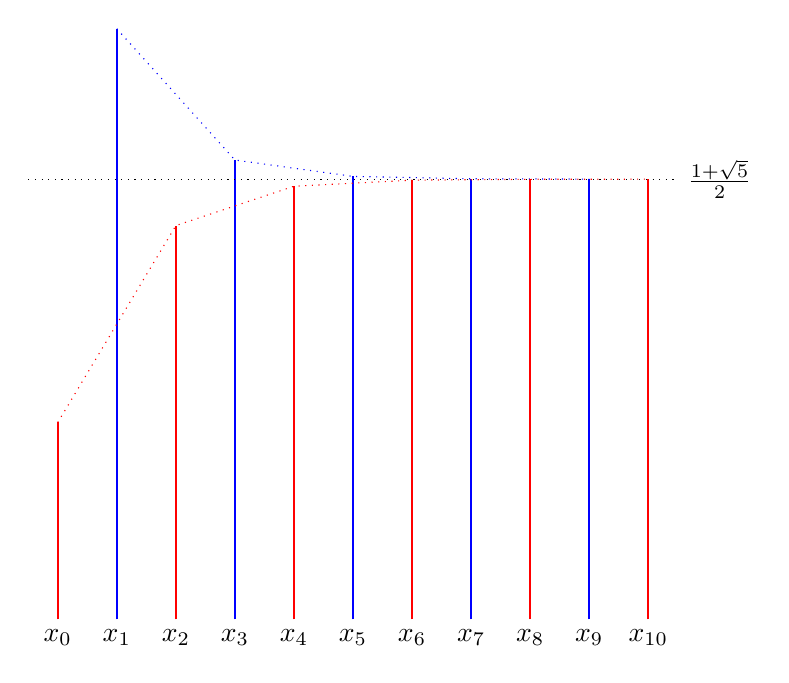
\begin{tikzpicture}[x=0.75cm, y=5cm]
      \draw[thick,color=red] (0, 0) -- (0,1.000000-0.5);
      \draw[thick,color=blue] (1, 0) -- (1,2.000000-0.5);
      \draw[thick,color=red] (2, 0) -- (2,1.500000-0.5);
      \draw[thick,color=blue] (3, 0) -- (3,1.666667-0.5);
      \draw[thick,color=red] (4, 0) -- (4,1.600000-0.5);
      \draw[thick,color=blue] (5, 0) -- (5,1.625000-0.5);
      \draw[thick,color=red] (6, 0) -- (6,1.615385-0.5);
      \draw[thick,color=blue] (7, 0) -- (7,1.619048-0.5);
      \draw[thick,color=red] (8, 0) -- (8,1.617647-0.5);
      \draw[thick,color=blue] (9, 0) -- (9,1.618182-0.5);
      \draw[thick,color=red] (10, 0) -- (10,1.617978-0.5);

      \draw[dotted,color=blue] (1,2.000000-0.5) -- (3,1.666667-0.5) -- (5,1.625000-0.5) -- (7,1.619048-0.5) -- (9,1.618182-0.5);

      \draw[dotted,color=red] (0,1.000000-0.5) -- (2,1.500000-0.5) -- (4,1.600000-0.5) -- (6,1.615385-0.5) -- (8,1.617647-0.5) -- (10,1.617978-0.5);

      \draw (0,0) node[below] {$x_0$};
      \draw (1,0) node[below] {$x_1$};
      \draw (2,0) node[below] {$x_2$};
      \draw (3,0) node[below] {$x_3$};
      \draw (4,0) node[below] {$x_4$};
      \draw (5,0) node[below] {$x_5$};
      \draw (6,0) node[below] {$x_6$};
      \draw (7,0) node[below] {$x_7$};
      \draw (8,0) node[below] {$x_8$};
      \draw (9,0) node[below] {$x_9$};
      \draw (10,0) node[below] {$x_{10}$};

      \draw[dotted] (-0.5,1.618033-0.5) -- (10.5,1.618033-0.5);
      \draw (10.5,1.618033-0.5) node[right] {$\frac{1 + \sqrt{5}}{2}$};
    \end{tikzpicture}
  \end{center}

  \caption{Valores de $x_n = [a_0,\ldots,a_n]$ (el caso de $[1,1,1,\ldots]$)}
  \label{fig:xn-numero-aureo}
\end{figure}

\begin{proposicion}
  Para una fracción continua infinita $[a_0,a_1,a_2,\ldots]$ el valor
  correspondiente está definido de manera única por los números $a_n$ y es
  irracional.

  \begin{proof}
    Para la unicidad, observamos que $x_0 < \alpha < x_1$, es decir
    $a_0 < \alpha < a_0 + \frac{1}{a_1}$. Dado que $a_1 \ge 1$, esto implica
    que
    \begin{equation}
      \label{eqn:fraccion-continua-a0}
      a_0 = \lfloor \alpha\rfloor.
    \end{equation}
    Además, es fácil comprobar que
    \begin{equation}
      \label{eqn:fraccion-continua-formula-recursiva-infinita}
            [a_0,a_1,a_2,\ldots] = a_0 + \frac{1}{[a_1,a_2,\ldots]}.
    \end{equation}
    Usando \eqref{eqn:fraccion-continua-a0} y
    \eqref{eqn:fraccion-continua-formula-recursiva-infinita}, se ve por
    inducción sobre $n$ que el valor de una fracción continua define de manera
    única sus coeficientes:
    \[ [a_0,a_1,a_2,\ldots] = [b_0,b_1,b_2,\ldots] \iff
       a_n = b_n \text{ para todo }n. \]

    Ahora para ver que el valor correspondiente es irracional, escribamos como
    antes
    $$x_n = [a_0,a_1,\ldots,a_n] = \frac{p_n}{q_n}.$$
    Si $[a_0,a_1,a_2,\ldots] = \alpha$, entonces como hemos visto arriba,
    $x_n < \alpha < x_{n+1}$ para todo $n$. Ahora
    $$0 < |\alpha - x_n| < |x_{n+1} - x_n| = \frac{1}{q_{n+1}\,q_n}$$
    (véase \eqref{eqn:pn-qn-identities-2}). Multiplicando todo por $q_n$,
    se obtiene
    $$0 < |\alpha q_n - p_n| < \frac{1}{q_{n+1}}.$$
    Ahora supongamos que $\alpha = a/b$ es racional, donde $b > 0$. Se obtiene
    la desigualdad
    $$0 < |a q_n - b p_n| < \frac{b}{q_{n+1}}.$$
    Pero para $n$ suficientemente grande se tiene $\frac{b}{q_{n+1}} < 1$,
    y esto nos lleva a una contradicción.
  \end{proof}
\end{proposicion}

\subsection{Fracción continua asociada a un número irracional}

Sea $\alpha$ un número irracional. Pongamos
$$\alpha_0 = \alpha, \quad a_0 = \lfloor \alpha_0\rfloor,$$
y luego por inducción para $n \ge 1$
$$\alpha_n = \frac{1}{\alpha_{n-1} - a_{n-1}}, \quad a_n = \lfloor
\alpha_n\rfloor.$$ Por inducción se ve que los $\alpha_n$ son números
irracionales y $0 < \alpha_{n-1} - a_{n-1} < 1$, así que $a_n \ge 1$ para
$n \ge 1$. Esto nos da una fracción continua
$$[a_0,a_1,a_2,\ldots],$$
y de hecho su valor coincide con $\alpha$.

En efecto, se tiene para todo $n$
$$\alpha = [a_0, \alpha_1] = [a_0, a_1, \alpha_2] = \cdots = [a_0, a_1, \ldots, a_{n-1}, \alpha_n].$$
Usando \eqref{eqn:fraccion-finita-pn-qn}, podemos escribir
$$\alpha = \frac{\alpha_n \, p_{n-1} + p_{n-2}}{\alpha_n \, q_{n-1} + q_{n-2}}.$$
Luego,
\[ \alpha - [a_0,a_1,\ldots,a_{n-1}] =
   \frac{\alpha_n \, p_{n-1} + p_{n-2}}{\alpha_n \, q_{n-1} + q_{n-2}} - \frac{p_{n-1}}{q_{n-1}} =
   \frac{-(p_{n-1}\, q_{n-2} - p_{n-2} \, q_{n-1})}{q_{n-1} \, (\alpha_n \, q_{n-1} + q_{n-2})} =
   \frac{(-1)^{n+1}}{q_{n-1} \, (\alpha_n \, q_{n-1} + q_{n-2})} \xrightarrow{n\to\infty} 0. \]

Para resumir, hemos obtenido una biyección
\[ \{ \text{fracciones continuas infinitas }[a_0,a_1,a_2,\ldots] \}
   \leftrightarrow
   \{ \text{números reales irracionales} \}. \]

\begin{ejemplo}
  Para $\alpha = \pi$ el algoritmo general nos da
  \begin{align*}
    \alpha_0 & = \pi = 3.14..., & a_0 & = \lfloor \alpha_0\rfloor = 3,\\
    \alpha_1 & = \frac{1}{\alpha_0 - a_0} = \frac{1}{\pi-3} = 7.06..., & a_1 & = \lfloor \alpha_1\rfloor = 7,\\
    \alpha_2 & = \frac{1}{\alpha_1 - a_1} =  15.99..., & a_2 & = \lfloor \alpha_2\rfloor = 15,\\
    \alpha_3 & = \frac{1}{\alpha_2 - a_2} =  1.003..., & a_3 & = \lfloor \alpha_3\rfloor = 1.
  \end{align*}
  Luego,
  $$\pi = [3,7,15,1,\ldots].$$
  Las primeras aproximaciones son
  \begin{align*}
    3 + \frac{1}{7}                                 = \frac{22}{7}    & = 3.1428571\ldots,\\
    3 + \cfrac{1}{7 + \cfrac{1}{15}}                = \frac{333}{106} & = 3.1415094\ldots,\\
    3 + \cfrac{1}{7 + \cfrac{1}{15 + \cfrac{1}{1}}} = \frac{355}{113} & = 3.1415929\ldots
  \end{align*}
  La aproximación $\frac{22}{7}$ era conocida a Arquímedes, mientras que
  $\frac{355}{113}$ fue descubierta por los matemáticos
  chinos\footnote{\url{https://en.wikipedia.org/wiki/Milü}}.
\end{ejemplo}

\begin{shaded}
  En PARI/GP la función \texttt{contfrac($\alpha$)} calcula la fracción continua
  para $\alpha$. Por ejemplo,
\begin{verbatim}
? contfrac(Pi)
% = [3, 7, 15, 1, 292, 1, 1, 1, 2, 1, 3, 1, 14, 2, 1, 1, 2, 2, 2, 2,
     1, 84, 2, 1, 1, 15, 3, 13, 1, 4, 2, 6, 6]
? contfracpnqn(%)
% =
[2646693125139304345 430010946591069243]

[ 842468587426513207 136876735467187340]

? %[1,2]/%[2,2] * 1.0
% = 3.1415926535897932384626433832795028929
? % - Pi
% = 8.663606142479168328 E-36

? contfrac (exp(1))
% = [2, 1, 2, 1, 1, 4, 1, 1, 6, 1, 1, 8, 1, 1, 10, 1, 1, 12, 1, 1, 14,
     1, 1, 16, 1, 1, 18, 1, 1, 20, 1, 1, 22, 1, 1, 24, 1, 1, 26, 2]
\end{verbatim}

  La fórmula curiosa
  $$e = [2, 1, 2, 1, 1, 4, 1, 1, 6, 1, 1, 8, 1, 1, 10, \ldots]$$
  fue descubierta por Euler; véase \cite{Sandifer-2006}, \cite{Olds-1970}, y
  \cite{Cohn-2006}. En particular, con esta fracción continua Euler estableció
  la irracionalidad de «su número» $e$.

  La fracción continua para $\pi$ no cumple ningún patrón aparente.
\end{shaded}

Las aproximaciones $\frac{p_n}{q_n}$ que salen de la fracción continua son las
mejores posibles en cierto sentido. A saber, si tenemos
$$\Bigl|\alpha - \frac{a}{b}\Bigr| < \Bigl|\alpha - \frac{p_n}{q_n}\Bigr|,$$
entonces $b > q_n$. Esto se deduce del siguiente resultado
(recuerde que $q_{n+1} > q_n$).

\begin{proposicion}
  Si $|\alpha b - a| < |\alpha q_n - p_n|$, entonces $b \ge q_{n+1}$.

  \begin{proof}
    Supongamos que $b < q_{n+1}$. Consideremos el sistema de ecuaciones
    lineales
    \[ \left\{\begin{array}{rcl}
      x q_n + y q_{n+1} & = & b, \\
      x p_n + y p_{n+1} & = & a.
    \end{array}\right. \]
    Aquí $\det \begin{pmatrix}
      q_n & q_{n+1} \\
      p_n & p_{n+1}
    \end{pmatrix} = \pm 1$, así que existe una solución única
    $x,y\in \ZZ$, donde $(x,y) \ne (0,0)$. De hecho, bajo nuestras hipótesis,
    $x\ne 0$ e $y \ne 0$. Efectivamente, si $x = 0$, entonces nos queda
    $b = y q_{n+1} \ge q_{n+1}$, que no es el caso. Por otra parte, si $y = 0$,
    entonces $x \ne 0$, y se tiene
    $$|\alpha b - a| = |x|\cdot |\alpha q_n - p_n| \ge |\alpha q_n - p_n|.$$

    Notamos que $x$ e $y$ necesariamente tienen diferentes signos: si $y < 0$,
    entonces $x = \frac{b - y q_{n+1}}{q_n} > 0$. De manera similar, si $y > 0$,
    entonces $x < 0$ por nuestra hipótesis de que $b < q_{n+1}$. Los números
    $\alpha q_n - p_n$ y $\alpha q_{n+1} - p_{n+1}$ también tienen diferentes
    signos: si $n$ es par, entonces
    $\frac{p_n}{q_n} < \alpha < \frac{p_{n+1}}{q_{n+1}}$,
    y si $n$ es impar, entonces
    $\frac{p_{n+1}}{q_{n+1}} < \alpha < \frac{p_n}{q_n}$.

    Esto implica que $x\,(\alpha q_n - p_n)$ e
    $y\,(\alpha q_{n+1} - p_{n+1})$ tienen el mismo signo, y luego
    \[ |\alpha b - a| =
       |x|\cdot |\alpha q_n - p_n| + |y|\cdot |\alpha q_{n+1} - p_n| >
       |\alpha q_n - p_n|. \qedhere \]
  \end{proof}
\end{proposicion}

\begin{corolario}
  \label{cor:mejor-aproximacion-por-pn/qn}
  Si $\Bigl|\alpha - \frac{a}{b}\Bigr| < \frac{1}{2b^2}$, entonces
  $\frac{a}{b} = \frac{p_n}{q_n}$ para algún $n$.

  \begin{proof}
    La sucesión $(q_n)$ es creciente, así que para algún $n$ se tiene
    $q_n \le b < q_{n+1}$. Según la proposición anterior, tenemos entonces
    $$|\alpha q_n - p_n| \le |\alpha b - a| < \frac{1}{2b},$$
    y luego
    $$\Bigl|\alpha - \frac{p_n}{q_n}\Bigr| < \frac{1}{2b q_n}.$$

    Ahora ocupando la desigualdad triangular,
    \[ \Bigl|\frac{a}{b} - \frac{p_n}{q_n}\Bigr| \le
       \Bigl|\alpha - \frac{a}{b}\Bigr| + \Bigl|\alpha - \frac{p_n}{q_n}\Bigr|
       < \frac{1}{2b^2} + \frac{1}{2b q_n}. \]
    Por otra parte, si $\frac{a}{b} \ne \frac{p_n}{q_n}$, entonces
    \[ \Bigl|\frac{a}{b} - \frac{p_n}{q_n}\Bigr| =
       \frac{|a q_n - b p_n|}{b q_n} \ge \frac{1}{b q_n}. \]
    Todo esto nos lleva a la desigualdad
    $$\frac{1}{b q_n} < \frac{1}{2b^2} + \frac{1}{2b q_n},$$
    de donde $b < q_n$, pero esto contradice nuestra hipótesis.
  \end{proof}
\end{corolario}

\subsection{Fracciones continuas periódicas}

\begin{definicion}
  Se dice que una fracción continua $\alpha = [a_0,a_1,a_2,\ldots]$ es
  \textbf{periódica} si existen números naturales $n_0$ y $k \ge 1$ tales que
  $a_n = a_{n+k}$ para todo $n \ge n_0$. En este caso se escribe
  $$\alpha = [a_0,a_1,\ldots,a_{n_0-1}, \overline{a_{n_0}, \ldots, a_{n_0+k-1}}].$$

  Si $n_0 = 0$; es decir, si $\alpha = [\overline{a_0,a_1,\ldots,a_{k-1}}]$,
  se dice que la fracción continua es \textbf{puramente periódica}.
\end{definicion}

\begin{ejemplo}
  Evaluemos la fracción periódica $[\overline{1,2,3}]$. La periodicidad nos da
  la relación
  $$\alpha = 1 + \cfrac{1}{2 + \cfrac{1}{3 + \cfrac{1}{\alpha}}}.$$
  Esta relación corresponde a la ecuación cuadrática
  $$7 \alpha^2 - 8\alpha - 3 = 0,$$
  de donde se obtiene
  \[ \alpha = \frac{4 + \sqrt{37}}{7}. \qedhere \]
\end{ejemplo}

\begin{proposicion}
  \label{prop:fraccion-periodica=>cuadratico}
  Si la fracción continua para $\alpha$ es periódica, entonces $\alpha$ es un
  número cuadrático irracional: se tiene $[\QQ (\alpha) : \QQ] = 2$.

  \begin{proof}
    Primero, si $\alpha = [\overline{a_0,a_1,\ldots,a_{k-1}}]$ es una fracción
    puramente periódica, entonces
    $$\alpha = [a_0,\ldots,a_{k-1},\alpha] = \frac{\alpha\,p_{k-1} + p_{k-2}}{\alpha\,q_{k-1} + q_{k-2}},$$
    lo que nos da una ecuación cuadrática
    $$q_{k-1}\,\alpha^2 + (q_{k-2} - p_{k-1})\,\alpha - p_{k-2} = 0.$$

    En general, podemos escribir $\alpha = [a_0,\ldots,a_{k-1},\beta]$, donde
    $\beta$ es la parte puramente periódica, y luego
    \[ \alpha = \frac{\beta\,p_{k-1} + p_{k-2}}{\beta\,q_{k-1} + q_{k-2}} \in \QQ (\beta). \qedhere \]
  \end{proof}
\end{proposicion}

Resulta que también se cumple la otra implicación: si $\alpha$ es un número
cuadrático, entonces la fracción continua correspondiente es periódica.
Veamos primero un ejemplo.

\begin{ejemplo}
  Para $\alpha = \sqrt{11}$ calculamos
  \begin{align*}
    \alpha_0 & = \sqrt{11} = 3.31\ldots, & a_0 & = \lfloor \alpha_0\rfloor = 3,\\
    \alpha_1 & = \frac{1}{\alpha_0 - a_0} = \frac{3 + \sqrt{11}}{2} = 3.15\ldots, & a_1 & = \lfloor \alpha_1\rfloor = 3,\\
    \alpha_2 & = \frac{1}{\alpha_1 - a_1} = 3 + \sqrt{11} = 6.31\ldots, & a_2 & = \lfloor \alpha_2\rfloor = 6,\\
    \alpha_3 & = \frac{1}{\alpha_2 - a_2} = \cfrac{1}{\sqrt{11} - 3} = \alpha_1, & a_3 & = a_1.
  \end{align*}
  Se ve que los cálculos se vuelven periódicos y el resultado es
  $$\sqrt{11} = [3, \, \overline{3,6}] = 3 + \cfrac{1}{3 + \cfrac{1}{6 + \cfrac{1}{3 + \cfrac{1}{6 + \cdots}}}}$$

  Las aproximaciones correspondientes son
  \begin{align*}
              [3,3] & = 3.33333333\ldots\\
            [3,3,6] & = 3.31578947\ldots\\
          [3,3,6,3] & = 3.31666666\ldots\\
        [3,3,6,3,6] & = 3.31662269\ldots\\
      [3,3,6,3,6,3] & = 3.31662489\ldots\\
                    & \cdots \\  
          \sqrt{11} & = 3.31662479\ldots \qedhere
  \end{align*}
\end{ejemplo}

\pdfbookmark{Clase 24 (09/11/20)}{clase-24}
\marginpar{\small Clase 24 \\ 09/11/20}
\begin{teorema}[Lagrange]
  La fracción continua de $\alpha$ es periódica si y solamente si
  $[\QQ (\alpha) : \QQ] = 2$.

  \begin{proof}[Demostración (\cite{Steinig-1992})]
    Ya lo probamos en una dirección. Ahora para un número cuadrático $\alpha$
    hay que ver que $\alpha_m = \alpha_n$ para algunos $m \ne n$. Por la
    hipótesis sobre $\alpha$, su polinomio mínimo
    $$f (x) = A\,x^2 + B\,x + C$$
    tiene discriminante
    $$\Delta = \Delta (f) = B^2 - 4 A C,$$
    donde $\Delta > 0$ (porque $\alpha$ es real) y $\Delta$ no es un cuadrado.
    Por inducción podemos definir una sucesión de polinomios cuadráticos
    $$f_n (x) = A_n\,x^2 + B_n\,x + C_n \in \ZZ [x]$$
    que cumplen
    $$f_n (\alpha_n) = 0, \quad \Delta (f_n) = \Delta.$$
    Para $n = 0$ tomamos $f_0 = f$. Para el paso inductivo, no es difícil
    comprobar que
    $$\alpha_{n+1}^2 \, f_n \Bigl(a_n + \frac{1}{\alpha_{n+1}}\Bigr) = \alpha_{n+1}^2 \, f_n (\alpha_n) = 0$$
    corresponde a la ecuación cuadrática
    \[ f_{n+1} (\alpha_{n+1}) = 0, \quad
       f_{n+1} (x) = A_{n+1}\,x^2 + B_{n+1}\,x + C_{n+1}, \]
    donde
    \begin{equation}
      \label{eqn:Lagrange-An-Bn-Cn}
      A_{n+1} = a_n^2\,A_n + a_n\,B_n + C_n, \quad
      B_{n+1} = 2\,a_n\,A_n + B_n, \quad
      C_{n+1} = A_n.
    \end{equation}
    Un cálculo directo demuestra que
    $$\Delta (f_{n+1}) = \Delta (f_n).$$

    Notamos que la sucesión $(A_n)$ cambia su signo un número infinito de
    veces. Por ejemplo, si $A_n > 0$ para todo $n$ suficientemente grande,
    entonces de \eqref{eqn:Lagrange-An-Bn-Cn} se ve que también $B_n, C_n > 0$
    para $n$ suficientemente grande. Pero $\alpha_n > 0$ para $n \ge 1$, y en
    este caso tendríamos
    $$f_n (\alpha_n) = A_n\,\alpha_n^2 + B_n\,\alpha_n + C_n > 0.$$

    Entonces, para un número infinito de $n$ se tiene
    $A_n\,A_{n-1} = A_n\,C_n < 0$, y en este caso el discriminante
    $$\Delta (f_n) = \Delta = B_n^2 - 4\,A_n\,C_n$$
    nos da la cota
    $$|B_n| < \sqrt{\Delta}, \quad |A_n|, |C_n| \le \frac{1}{4}\,\Delta.$$
    Puesto que esto se cumple para un número infinito de $n$, habrá $m\ne n$
    tales que $f_m = f_n$ y $\alpha_m = \alpha_n$.
  \end{proof}
\end{teorema}

También sería interesante investigar cuándo la fracción continua es
\emph{puramente} periódica. La caracterización es la siguiente.

\begin{teorema}
  Sea $\alpha \in \QQ (\sqrt{d})$ un número real cuadrático. Denotemos por
  $\overline{\cdot}$ el automorfismo no trivial $\sqrt{d} \mapsto -\sqrt{d}$.
  La fracción continua para $\alpha$ es puramente periódica si y solamente si
  $\alpha > 1$ y $-1 < \overline{\alpha} < 0$.

  \begin{proof}
    Supongamos primero que la fracción continua para $\alpha$ es puramente
    periódica y $\alpha = [\overline{a_0,a_1,\ldots,a_{k-1}}]$. En todo caso se
    cumple $q_n \ge 1$, y luego, $a_0 = a_k \ge 1$ implica por inducción que
    también ${p_n = a_n\,p_{n-1} + p_{n-2} \ge 1}$ para todo $n$. Entonces,
    $\alpha = \lim_{n\to\infty} \frac{p_n}{q_n} > 1$. Como ya notamos en
    \ref{prop:fraccion-periodica=>cuadratico}, $\alpha$, y luego
    $\overline{\alpha}$, es una raíz del polinomio cuadrático
    $$f (x) = q_{k-1}\,\alpha^2 + (q_{k-2} - p_{k-1})\,\alpha - p_{k-2} = 0.$$
    Es fácil verificar que $f (0) < 0$ y $f (-1) > 0$, así que $f$ tiene una raíz
    entre $-1$ y $0$, y luego $-1 < \overline{\alpha} < 0$.

    \vspace{1em}

    En la otra dirección, supongamos que $\alpha > 1$ y
    $-1 < \overline{\alpha} < 0$. Esto implica por inducción que $\alpha_n > 1$
    y $-1 < \overline{\alpha_n} < 0$ para todo $n \ge 0$. Notamos que
    \[ \alpha_n = a_n + \frac{1}{\alpha_{n+1}} \Longrightarrow
       \overline{\alpha_n} = a_n + \frac{1}{\overline{\alpha_{n+1}}}. \]
    Ahora la desigualdad $-1 < \overline{\alpha_n} < 0$ puede ser escrita como
    $$0 < -\frac{1}{\overline{\alpha_{n+1}}} - a_n < 1,$$
    de donde
    $$a_n = \left\lfloor-\frac{1}{\overline{\alpha_{n+1}}}\right\rfloor.$$

    Dado que $\alpha$ es un número cuadrático, la sucesión $(\alpha_n)$ es
    periódica, y existe $k$ tal que $\alpha_n = \alpha_{n+k}$ para $n$
    \emph{suficientemente grande}, y nos gustaría ver que esto es cierto para
    $n = 0$. Tenemos
    \[ a_{n-1} = \left\lfloor-\frac{1}{\overline{\alpha_n}}\right\rfloor =
       \left\lfloor-\frac{1}{\overline{\alpha_{n+k}}}\right\rfloor = a_{n-1+k}. \]
    De aquí
    \[ \alpha_{n-1} = a_{n-1} + \frac{1}{\alpha_n} =
       a_{n-1+k} + \frac{1}{\alpha_{n+k}} = \alpha_{n-1+k}. \]
    Aplicando este razonamiento, llegaremos a $\alpha_0 = \alpha_k$.
  \end{proof}
\end{teorema}

\begin{corolario}
  Sea $d > 1$ un entero que no es un cuadrado. Entonces,
  $$\sqrt{d} = [\lfloor\sqrt{d}\rfloor, \overline{a_1,\ldots,a_k}],$$
  donde $a_k = 2\lfloor\sqrt{d}\rfloor$.

  \begin{proof}
    Notamos que para el número $\alpha = \sqrt{d} + \lfloor\sqrt{d}\rfloor$
    se cumple $\alpha > 0$ y $-1 < \overline{\alpha} < 0$, así que la fracción
    continua de $\alpha$ es puramente periódica:
    $\alpha = [\overline{a_0,a_1,\ldots,a_{k-1}}]$,
    donde $a_0 = a_k = \lfloor\alpha\rfloor = 2\lfloor\sqrt{d}\rfloor$. Luego,
    \[ \sqrt{d} = \alpha - \lfloor\sqrt{d}\rfloor =
       [\lfloor\sqrt{d}\rfloor, \overline{a_1,\ldots,a_{k-1},a_k}]. \qedhere \]
  \end{proof}
\end{corolario}

\begin{comentario}
  El número más pequeño $k$ tal que
  $\sqrt{d} = [\lfloor\sqrt{d}\rfloor, \overline{a_1,\ldots,a_k}]$ se llama el
  \textbf{período}. El mismo Lagrange obtuvo una cota $< 2d$, pero los cálculos
  sugieren la cota $O (\sqrt{d})$. Véase las referencias en
  \url{https://oeis.org/A003285} para más detalles.
\end{comentario}

En la figura \ref{fig:fracciones-continuas-para-sqrt-d} se encuentran las
fracciones continuas para $\sqrt{d}$, donde $d < 100$.

\begin{figure}
  \begin{multicols}{2}
    \begin{align*}
      \sqrt{2} & = [1,\overline{2}] \\
      \sqrt{3} & = [1,\overline{1,2}] \\
      \sqrt{5} & = [2,\overline{4}] \\
      \sqrt{6} & = [2,\overline{2,4}] \\
      \sqrt{7} & = [2,\overline{1,1,1,4}] \\
      \sqrt{10} & = [3,\overline{6}] \\
      \sqrt{11} & = [3,\overline{3,6}] \\
      \sqrt{13} & = [3,\overline{1,1,1,1,6}] \\
      \sqrt{14} & = [3,\overline{1,2,1,6}] \\
      \sqrt{15} & = [3,\overline{1,6}] \\
      \sqrt{17} & = [4,\overline{8}] \\
      \sqrt{19} & = [4,\overline{2,1,3,1,2,8}] \\
      \sqrt{21} & = [4,\overline{1,1,2,1,1,8}] \\
      \sqrt{22} & = [4,\overline{1,2,4,2,1,8}] \\
      \sqrt{23} & = [4,\overline{1,3,1,8}] \\
      \sqrt{26} & = [5,\overline{10}] \\
      \sqrt{29} & = [5,\overline{2,1,1,2,10}] \\
      \sqrt{30} & = [5,\overline{2,10}] \\
      \sqrt{31} & = [5,\overline{1,1,3,5,3,1,1,10}] \\
      \sqrt{33} & = [5,\overline{1,2,1,10}] \\
      \sqrt{34} & = [5,\overline{1,4,1,10}] \\
      \sqrt{35} & = [5,\overline{1,10}] \\
      \sqrt{37} & = [6,\overline{12}] \\
      \sqrt{38} & = [6,\overline{6,12}] \\
      \sqrt{39} & = [6,\overline{4,12}] \\
      \sqrt{41} & = [6,\overline{2,2,12}] \\
      \sqrt{42} & = [6,\overline{2,12}] \\
      \sqrt{43} & = [6,\overline{1,1,3,1,5,1,3,1,1,12}] \\
      \sqrt{46} & = [6,\overline{1,3,1,1,2,6,2,1,1,3,1,12}] \\
      \sqrt{47} & = [6,\overline{1,5,1,12}]
    \end{align*}

    \begin{align*}
      \sqrt{51} & = [7,\overline{7,14}] \\
      \sqrt{53} & = [7,\overline{3,1,1,3,14}] \\
      \sqrt{55} & = [7,\overline{2,2,2,14}] \\
      \sqrt{57} & = [7,\overline{1,1,4,1,1,14}] \\
      \sqrt{58} & = [7,\overline{1,1,1,1,1,1,14}] \\
      \sqrt{59} & = [7,\overline{1,2,7,2,1,14}] \\
      \sqrt{61} & = [7,\overline{1,4,3,1,2,2,1,3,4,1,14}] \\
      \sqrt{62} & = [7,\overline{1,6,1,14}] \\
      \sqrt{65} & = [8,\overline{16}] \\
      \sqrt{66} & = [8,\overline{8,16}] \\
      \sqrt{67} & = [8,\overline{5,2,1,1,7,1,1,2,5,16}] \\
      \sqrt{69} & = [8,\overline{3,3,1,4,1,3,3,16}] \\
      \sqrt{70} & = [8,\overline{2,1,2,1,2,16}] \\
      \sqrt{71} & = [8,\overline{2,2,1,7,1,2,2,16}] \\
      \sqrt{73} & = [8,\overline{1,1,5,5,1,1,16}] \\
      \sqrt{74} & = [8,\overline{1,1,1,1,16}] \\
      \sqrt{77} & = [8,\overline{1,3,2,3,1,16}] \\
      \sqrt{78} & = [8,\overline{1,4,1,16}] \\
      \sqrt{79} & = [8,\overline{1,7,1,16}] \\
      \sqrt{82} & = [9,\overline{18}] \\
      \sqrt{83} & = [9,\overline{9,18}] \\
      \sqrt{85} & = [9,\overline{4,1,1,4,18}] \\
      \sqrt{86} & = [9,\overline{3,1,1,1,8,1,1,1,3,18}] \\
      \sqrt{87} & = [9,\overline{3,18}] \\
      \sqrt{89} & = [9,\overline{2,3,3,2,18}] \\
      \sqrt{91} & = [9,\overline{1,1,5,1,5,1,1,18}] \\
      \sqrt{93} & = [9,\overline{1,1,1,4,6,4,1,1,1,18}] \\
      \sqrt{94} & = [9,\overline{1,2,3,1,1,5,1,8,1,5,1,1,3,2,1,18}] \\
      \sqrt{95} & = [9,\overline{1,2,1,18}] \\
      \sqrt{97} & = [9,\overline{1,5,1,1,1,1,1,1,5,1,18}]
    \end{align*}
  \end{multicols}

  \caption{Fracciones continuas para $\sqrt{d}$, donde $d < 100$}
  \label{fig:fracciones-continuas-para-sqrt-d}
\end{figure}

%%%%%%%%%%%%%%%%%%%%%%%%%%%%%%%%%%%%%%%%%%%%%%%%%%%%%%%%%%%%%%%%%%%%%%%%%%%%%%%%

\section{Volviendo a la ecuación de Pell}

La ecuación de Pell $x^2 - dy^2 = \pm 1$ está relacionada con la fracción
continua de $\sqrt{d}$ de la siguiente manera.

\begin{proposicion}
  Toda solución entera con $x,y > 0$ de la ecuación $x^2 + dy^2 = \pm 1$ tiene
  forma $(x,y) = (p_n,q_n)$ para algún $n$, donde los $\frac{p_n}{q_n}$ vienen
  de la fracción continua para $\sqrt{d}$.

  \begin{proof}
    De manera un poco más general, sean $x,y$ enteros positivos tales que
    $\gcd (x,y) = 1$ y $s,t$ números reales tales que
    \[ x^2 - ry^2 = s, \quad
       0 < s < \sqrt{r}, \quad
       \sqrt{r}\text{ es irracional}. \]

    Escribiendo $(x - y\sqrt{r})\,(x + y\sqrt{r}) = s$, se obtiene
    la desigualdad
    \[ \frac{x}{y} - \sqrt{r} = \frac{s}{y\,(x + y\sqrt{r})} <
    \frac{\sqrt{r}}{y\,(x + y\sqrt{r})} =
    \cfrac{1}{y^2\,\Bigl(\cfrac{x}{y\sqrt{r}} + 1\Bigr)} <
    \frac{1}{2y^2}, \]
    usando que $\frac{x}{y\sqrt{r}} > 1$, como consecuencia de
    $\frac{x}{y} - \sqrt{r} > 0$. Ahora, dado que
    $$\Bigl|\frac{x}{y} - \sqrt{r}\Bigr| < \frac{1}{2y^2},$$
    el resultado de \ref{cor:mejor-aproximacion-por-pn/qn} nos dice que
    $\frac{x}{y} = \frac{p_n}{q_n}$ para algún $n$, donde los $\frac{p_n}{q_n}$
    salen de la fracción continua para $\sqrt{r}$.

    Si nos interesa la ecuación $x^2 - dy^2 = +1$, basta aplicar nuestro
    argumento a $r = d$ y $s = 1$. Por otra parte, si la ecuación es
    $x^2 - dy^2 = -1$, entonces podemos tomar $r = s = \frac{1}{d}$. En este
    caso la ecuación será
    $$x^2 - \frac{1}{d}\,y^2 = \frac{1}{d} \iff y^2 - dx^2 = -1.$$
    Tenemos $\frac{x}{y} = \frac{p_n'}{q_n'}$ para algún $n$, donde los
    $\frac{p_n'}{q_n'}$ salen de la fracción continua para $\frac{1}{\sqrt{d}}$.
    Pero no es difícil verificar que
    $\frac{p_n'}{q_n'} = \frac{q_{n-1}}{p_{n-1}}$, donde las fracciones
    $\frac{p_n}{q_n}$ vienen de $\sqrt{d}$ (¡ejercicio!).
  \end{proof}
\end{proposicion}

Ahora la pregunta es cuándo $\frac{p_n}{q_n}$ nos da una solución de la ecuación
de Pell. Para verlo, nos conviene describir la fracción continua de $\sqrt{d}$
de manera más explícita.

\begin{proposicion}
  Consideremos la fracción continua
  $$\sqrt{d} = [a_0, \overline{a_1,\ldots,a_k}],$$
  donde $k$ es el periodo. Como antes, consideremos $\alpha_0 = \alpha$ y
  \[ a_n = \lfloor\alpha_n\rfloor, \quad
     \alpha_{n+1} = \frac{1}{\alpha_n - a_n}. \]

  \begin{enumerate}
  \item[1)] Se tiene $\alpha_n = \frac{A_n + \sqrt{d}}{B_n}$, donde
    $A_0 = 0$, $B_0 = 1$, y
    \begin{equation}
      \label{eq:An-Bn-para-sqrt-d}
      A_{n+1} = a_n\,B_n - A_n, \quad
      B_{n+1} = \frac{d - A_{n+1}^2}{B_n} \in \ZZ.
    \end{equation}

  \item[2)] $B_n = +1$ si y solamente si $k \mid n$.

  \item[3)] $B_n \ne -1$ para ningún $n$.

  \item[4)] Para todo $n$ se tiene $p_n^2 - d\,q_n^2 = (-1)^{n+1}\,B_{n+1}$.
  \end{enumerate}

  \begin{proof}
    La parte 1) se deja como un ejercicio.

    En la parte 2), primero consideremos $B_k$, donde $k$ es el período.
    Tenemos $\alpha_{k+1} = \alpha_1$, y luego
    \[ A_{k+1} = A_1 = \lfloor\sqrt{d}\rfloor, \quad
       B_{k+1} = \frac{d - A_{k+1}^2}{B_k} = B_1 = d - \lfloor\sqrt{d}\rfloor^2. \]
    Esto implica que $B_k = 1$. Viceversa, si $B_n = 1$ para algún $n$, entonces
    $\alpha_n = A_n + \sqrt{d}$, y podemos escribir
    ${\alpha = [a_0,a_1,\ldots,a_{n-1},\alpha_n]}$, donde el número $\alpha_n$
    tiene fracción continua puramente periódica, y por lo tanto
    ${-1 < \overline{\alpha_n} < 0}$. Esto implica que
    ${\sqrt{d} - 1 < A_n < \sqrt{d}}$, y luego $A_n = \lfloor\sqrt{d}\rfloor$.
    Ahora ${\alpha_n = \sqrt{d} + \lfloor\sqrt{d}\rfloor = \alpha_1}$, y esto es
    posible precisamente si $k \mid n$.

    En la parte 3) de manera similar, si $B_n = -1$, entonces
    ${\alpha_n = -A_n - \sqrt{d}}$ tiene fracción continua puramente periódica,
    y luego
    \[ \alpha_n > 1, ~ -1 < \overline{\alpha_n} < 0
       \iff
       -A_n - \sqrt{d} > 1, ~ -1 < -A_n + \sqrt{d} < 0, \]
    pero estas desigualdades implican que
    ${\sqrt{d} < A_n < -\sqrt{d} - 1}$. Contradicción.

    En fin, en 4) escribamos
    \[ \sqrt{d} = \alpha =
       \frac{\alpha_{n+1}\,p_n + p_{n-1}}{\alpha_{n+1}\,q_n + q_{n-1}} =
       \frac{(A_{n+1} + \sqrt{d})\,p_n + B_{n+1}\,p_{n-1}}{(A_{n+1} + \sqrt{d})\,q_n + B_{n+1}\,q_{n-1}}. \]
    Dejo al lector analizar la ecuación correspondiente en $\QQ (\sqrt{d})$,
    expresar de allí $A_{n+1}$ en términos de $B_{n+1}$ y verificar que nos
    queda
    \[ p_n^2 - d\,q_n^2 =
       (p_n\,q_{n-1} - p_{n-1}\,q_n)\,B_{n+1} = (-1)^{n+1}\,B_{n+1}. \qedhere. \]
  \end{proof}
\end{proposicion}

Entonces, hemos probado que las soluciones de la ecuación de Pell son
$(p_n,q_n)$ para algún $n$, y además que
$p_n^2 - d\,q_n^2 = (-1)^{n+1}\,B_{n+1}$. Aquí $B_{n+1} \ne -1$ y $B_{n+1} = +1$
si y solamente si $k \mid (n+1)$. Esto nos lleva al siguiente resultado.

\begin{teorema}
  Para un entero libre de cuadrados $d$ consideremos la fracción continua para
  $\sqrt{d}$. Si $k$ es el período, entonces las soluciones enteras positivas
  de la ecuación $x^2 - dy^2 = \pm 1$ tienen forma $(x,y) = (p_{kn-1}, q_{kn-1})$,
  donde $n = 1,2,3,\ldots$
\end{teorema}

\begin{ejemplo}
  Consideremos la ecuación $x^2 - 41\,y^2 = \pm 1$. En este caso primero
  calculamos la fracción continua $\sqrt{41} = [6, \overline{2,2,12}]$.
  Las soluciones no triviales son $(x,y) = (p_{3n-1}, q_{3n-1})$. En particular,
  la solución más pequeña será $(x,y) = (p_2,q_2) = (32,5)$.
  Efectivamente, verificamos que $32^2 - 41\cdot 5^2 = -1$.
\end{ejemplo}

\begin{ejemplo}
  Las soluciones de la ecuación de Pell suelen ser bastante grandes, pero
  tenemos un algoritmo eficaz de entontrarlas. Por ejemplo, para la ecuación
  $x^2 - 151\,y^2 = \pm 1$, primero calculamos la fracción continua
  $$\sqrt{151} = [12, \overline{3, 2, 7, 1, 3, 4, 1, 1, 1, 11, 1, 1, 1, 4, 3, 1, 7, 2, 3, 24}]$$
  (no es difícil hacerlo con la computadora ocupando las fórmulas
  \eqref{eq:An-Bn-para-sqrt-d}).  Aquí el periodo es igual a $21$, y luego
  la solución más pequeña será $(p_{20},q_{20})$. Calculámosla con PARI/GP:
\begin{shaded}
\begin{verbatim}
? fr = [12,3,2,7,1,3,4,1,1,1,11,1,1,1,4,3,1,7,2,3,24];
? contfracpnqn(fr)
% = 
[41973615123 1728148040]

[ 3415764356  140634693]

? [p,q] = [%[1,2], %[2,2]]
% = [1728148040, 140634693]
? p^2 - 151*q^2
% = 1
\end{verbatim}
\end{shaded}
\end{ejemplo}

%%%%%%%%%%%%%%%%%%%%%%%%%%%%%%%%%%%%%%%%%%%%%%%%%%%%%%%%%%%%%%%%%%%%%%%%%%%%%%%%

\section{Unidades fundamentales en campos cuadráticos reales}

Consideremos un campo cuadrático real $K = \QQ (\sqrt{d})$. En este caso el
teorema de unidades nos dice que
$$\O_K^\times = \{ \pm 1 \} \times \langle u\rangle,$$
donde $u$ es la unidad fundamental. Nuestro objetivo será encontrarla de manera
explícita.

Si $d \equiv 1 \pmod{4}$, entonces
$\O_K = \ZZ \Bigl[\frac{1+\sqrt{d}}{2}\Bigr]$. Para una unidad
$v = a + b\,\frac{1+\sqrt{d}}{2} \in \O_K^\times$ tenemos
$$N_{K/\QQ} (v) = a^2 + ab + \frac{1 - d}{4}\,b^2 = \pm 1.$$
Si $d \equiv 1 \pmod{8}$, entonces considerando diferentes opciones mód $8$,
se ve que $b$ tiene que ser par en cualquier caso, así que
$v \in \ZZ [\sqrt{d}]^\times$. Por otra parte, si $d \equiv 5 \pmod{8}$, un
cálculo directo y tedioso demuestra que $v^3 \in \ZZ [\sqrt{d}]^\times$.
Todo esto significa lo siguiente.
\begin{itemize}
\item Si $d \equiv 2,3 \pmod{4}$ o $d \equiv 1 \pmod{8}$, entonces
  $\O_K^\times = \ZZ [\sqrt{d}]^\times$.

\item si $d \equiv 5 \pmod{8}$, entonces
  $[\O_K^\times : \ZZ [\sqrt{d}]^\times] = 1\text{ o }3$.
  Si $u$ es la unidad fundamental de $\ZZ [\sqrt{d}]^\times$, entonces para
  encontrar la unidad fundamental de $\O_K^\times$, basta resolver la ecuación
  $u^3 = v$ en $\O_K$. Si esta no tiene soluciones, entonces
  $\O_K^\times = \ZZ [\sqrt{d}]^\times$.
\end{itemize}
En cualquier caso, para encontrar las unidades en $\O_K$, bastará conocer las
unidades en $\ZZ [\sqrt{d}]$. Tenemos
\[ \{ x + y\sqrt{d} \mid x,y > 0, ~ x^2 - dy^2 = \pm 1 \} =
\{ u^n \mid n = 1,2,3,\ldots \}, \]
donde $u$ es la unidad fundamental de $\ZZ [\sqrt{d}]$, definida como la unidad
más pequeña tal que $u > 1$. Por otra parte, sabemos que las unidades de arriba
tienen forma $p_{kn-1} + q_{kn-1}\sqrt{d}$, donde $k$ es el período de la fracción
continua para $\sqrt{d}$. La más pequeña entre estas corresponde a $n = 1$, así
que
$$u = p_{k-1} + q_{k-1}\sqrt{d}.$$

\begin{ejemplo}
  Para $K = \QQ (\sqrt{2})$, empezamos por la fracción continua
  $\sqrt{2} = [1,\overline{2}]$. En este caso nos interesan $p_0 = 1$
  y $q_0 = 1$. Entonces, la unidad fundamental es $u = 1 + \sqrt{2}$.
\end{ejemplo}

\begin{ejemplo}
  Para $K = \QQ (\sqrt{5})$ tenemos $\sqrt{5} = [2,\overline{4}]$.
  En este caso $p_0 = 2$, $q_0 = 1$, así que la unidad fundamental de
  $\ZZ [\sqrt{5}]^\times$ es $u = 2 + \sqrt{5}$. El anillo de enteros
  es $\O_K = \ZZ \Bigl[\frac{1+\sqrt{5}}{2}\Bigr]$. Para
  $v = A + B\frac{1+\sqrt{5}}{2}$ consideremos la ecuación $v^3 = u$.
  Esta nos da
  \[ \left\{\begin{array}{rcl}
  A^3 + \frac{3}{2}\,A^2 B + \frac{9}{2}\,A B^2 + 2\,B^3 & = & 2,\\
  \frac{3}{2}\,A^2 B + \frac{3}{2}\,A B^2 + B^2 & = & 1.
  \end{array}\right. \]
  Se ve que $A = 0$, $B = 1$ nos da una solución, así que la unidad fundamental
  de $\O_K^\times$ es $v = \frac{1+\sqrt{5}}{2}$.
\end{ejemplo}

\begin{ejemplo}
  Consideremos $K = \QQ (\sqrt{13})$. En este caso
  $\sqrt{13} = [3, \overline{1,1,1,1,6}]$, y la unidad fundamental de
  $\ZZ [\sqrt{13}]^\times$ es $u = p_4 + q_4\sqrt{13} = 18 + 5\sqrt{13}$.
  Luego resolviendo la ecuación $v^3 = u$ en
  $\ZZ \Bigl[\frac{1+\sqrt{13}}{2}\Bigr]$ se obtiene
  la unidad fundamental $v = 1 + \frac{1 + \sqrt{13}}{2}$.
\end{ejemplo}

\begin{ejemplo}
  Consideremos $K = \QQ (\sqrt{37})$. Tenemos $\sqrt{37} = [6,\overline{12}]$,
  y entonces la unidad fundamental de $\ZZ [\sqrt{37}]^\times$ será
  $u = p_0 + q_0\sqrt{37} = 6 + \sqrt{37}$. Ahora la ecuación $v^3 = u$ en
  $\ZZ \Bigl[\frac{1+\sqrt{37}}{2}\Bigr]$ corresponde a
  \[ \left\{\begin{array}{rcl}
  A^3 + \frac{3}{2}\,A^2\,B + \frac{57}{2}\,A\,B^2 + 14\,B^3 & = & 6,\\
  \frac{3}{2}\,A^2\,B + \frac{3}{2}\,A B^2 + 5\,B^3 & = & 1.
  \end{array}\right. \]

  Escribamos la segunda ecuación como
  $$B\,(3\,A^2 + 3\,AB + 10\,B^2) = 2.$$
  De aquí se sigue que $B = \pm 1$ o $\pm 2$. Sustituyendo estos valores,
  se obtiene una ecuación cuadrática en $A$ que no tiene soluciones enteras.
  Entonces, $v^3 = u$ no tiene solución. Esto significa que
  $\O_K^\times = \ZZ [\sqrt{37}]^\times$, y la unidad fundamental es la misma
  $u$.
\end{ejemplo}

En la figura \ref{fig:unidades-fundamentales-cuadraticas} se encuentran las
unidades fundamentales en $\ZZ [\sqrt{d}]^\times$ y
$\ZZ \Bigl[\frac{1+\sqrt{d}}{2}\Bigr]^\times$ para $d < 100$.

\begin{figure}
  \begin{center}\def\arraystretch{1.65}\small
    \begin{tabular}{M{0.3cm}M{0.4cm}M{2.5cm}M{2.1cm}M{0.7cm}|M{0.3cm}M{0.4cm}M{3.3cm}M{2.4cm}M{0.7cm}}
      \hline
      $d$ & $d~(8)$ & $u \in \ZZ [\sqrt{d}]^\times$ & $v \in \ZZ \Bigl[\frac{1+\sqrt{d}}{2}\Bigr]^\times$ & $N (u)$ & $d$ & $d~(8)$ & $u \in \ZZ [\sqrt{d}]^\times$ & $v \in \ZZ \Bigl[\frac{1+\sqrt{d}}{2}\Bigr]^\times$ & $N (u)$ \\
      \hline
      $2$ & $2$ & $1 + \sqrt{2}$ & & $-1$ & $51$ & $3$ & $50 + 7\sqrt{51}$ & & $+1$ \\
      $3$ & $3$ & $2 + \sqrt{3}$ & & $+1$ & $53$ & $5$ & $182 + 25\sqrt{53}$ & $3 + \frac{1+\sqrt{53}}{2}$ & $-1$ \\
      $5$ & $5$ & $2 + \sqrt{5}$ & $\frac{1+\sqrt{5}}{2}$ & $-1$ & $55$ & $7$ & $89 + 12\sqrt{55}$ & & $+1$ \\
      $6$ & $6$ & $5 + 2\sqrt{6}$ & & $+1$ & $57$ & $1$ & $152 + 20\sqrt{57}$ & $152 + 20\sqrt{57}$ & $+1$ \\
      $7$ & $7$ & $8 + 3\sqrt{7}$ & & $+1$ & $58$ & $2$ & $99 + 13\sqrt{58}$ & & $-1$ \\
      $10$ & $2$ & $3 + \sqrt{10}$ & & $-1$ & $59$ & $3$ & $530 + 69\sqrt{59}$ & & $+1$ \\
      $11$ & $3$ & $10 + 3\sqrt{11}$ & & $+1$ & $61$ & $5$ & $29718 + 3805\sqrt{61}$ & $17 + 5\,\frac{1+\sqrt{61}}{2}$ & $-1$ \\
      $13$ & $5$ & $18 + 5\sqrt{13}$ & $1 + \frac{1+\sqrt{13}}{2}$ & $-1$ & $62$ & $6$ & $63 + 8\sqrt{62}$ & & $+1$ \\
      $14$ & $6$ & $15 + 4\sqrt{14}$ & & $+1$ & $65$ & $1$ & $8 + \sqrt{65}$ & $8 + \sqrt{65}$ & $-1$ \\
      $15$ & $7$ & $4 + \sqrt{15}$ & & $+1$ & $66$ & $2$ & $65 + 8\sqrt{66}$ & & $+1$ \\
      $17$ & $1$ & $4 + \sqrt{17}$ & $4 + \sqrt{17}$ & $-1$ & $67$ & $3$ & $48842 + 5967\sqrt{67}$ & & $+1$ \\
      $19$ & $3$ & $170 + 39\sqrt{19}$ & & $+1$ & $69$ & $5$ & $7775 + 936\sqrt{69}$ & $11 + 3\,\frac{1+\sqrt{69}}{2}$ & $+1$ \\
      $21$ & $5$ & $55 + 12\sqrt{21}$ & $2 + \frac{1+\sqrt{21}}{2}$ & $+1$ & $70$ & $6$ & $251 + 30\sqrt{70}$ & & $+1$ \\
      $22$ & $6$ & $197 + 42\sqrt{22}$ & & $+1$ & $71$ & $7$ & $3480 + 413\sqrt{71}$ & & $+1$ \\
      $23$ & $7$ & $24 + 5\sqrt{23}$ & & $+1$ & $73$ & $1$ & $1068 + 125\sqrt{73}$ & $1068 + 125\sqrt{73}$ & $-1$ \\
      $26$ & $2$ & $5 + \sqrt{26}$ & & $-1$ & $74$ & $2$ & $43 + 5\sqrt{74}$ & & $-1$ \\
      $29$ & $5$ & $70 + 13\sqrt{29}$ & $2 + \frac{1+\sqrt{29}}{2}$ & $-1$ & $77$ & $5$ & $351 + 40\sqrt{77}$ & $4 + \frac{1+\sqrt{77}}{2}$ & $+1$ \\
      $30$ & $6$ & $11 + 2\sqrt{30}$ & & $+1$ & $78$ & $6$ & $53 + 6\sqrt{78}$ & & $+1$ \\
      $31$ & $7$ & $1520 + 273\sqrt{31}$ & & $+1$ & $79$ & $7$ & $80 + 9\sqrt{79}$ & & $+1$ \\
      $33$ & $1$ & $23 + 4\sqrt{33}$ & $23 + 4\sqrt{33}$ & $+1$ & $82$ & $2$ & $9 + \sqrt{82}$ & & $-1$ \\
      $34$ & $2$ & $35 + 6\sqrt{34}$ & & $+1$ & $83$ & $3$ & $82 + 9\sqrt{83}$ & & $+1$ \\
      $35$ & $3$ & $6 + \sqrt{35}$ & & $+1$ & $85$ & $5$ & $378 + 41\sqrt{85}$ & $4 + \frac{1+\sqrt{85}}{2}$ & $-1$ \\
      $37$ & $5$ & $6 + \sqrt{37}$ & $6 + \sqrt{37}$ & $-1$ & $86$ & $6$ & $10405 + 1122\sqrt{86}$ & & $+1$ \\
      $38$ & $6$ & $37 + 6\sqrt{38}$ & & $+1$ & $87$ & $7$ & $28 + 3\sqrt{87}$ & & $+1$ \\
      $39$ & $7$ & $25 + 4\sqrt{39}$ & & $+1$ & $89$ & $1$ & $500 + 53\sqrt{89}$ & $500 + 53\sqrt{89}$ & $-1$ \\
      $41$ & $1$ & $32 + 5\sqrt{41}$ & $32 + 5\sqrt{41}$ & $-1$ & $91$ & $3$ & $1574 + 165\sqrt{91}$ & & $+1$ \\
      $42$ & $2$ & $13 + 2\sqrt{42}$ & & $+1$ & $93$ & $5$ & $12151 + 1260\sqrt{93}$ & $13 + 3\,\frac{1+\sqrt{93}}{2}$ & $+1$ \\
      $43$ & $3$ & $3482 + 531\sqrt{43}$ & & $+1$ & $94$ & $6$ & $2143295 + 221064\sqrt{94}$ & & $+1$ \\
      $46$ & $6$ & $24335 + 3588\sqrt{46}$ & & $+1$ & $95$ & $7$ & $39 + 4\sqrt{95}$ & & $+1$ \\
      $47$ & $7$ & $48 + 7\sqrt{47}$ & & $+1$ & $97$ & $1$ & $5604 + 569\sqrt{97}$ & $5604 + 569\sqrt{97}$ & $-1$ \\
    \end{tabular}
  \end{center}

  \caption{Unidades fundamentales en $\ZZ [\sqrt{d}]^\times$ y $\ZZ \Bigl[\frac{1+\sqrt{d}}{2}\Bigr]^\times$, donde $d < 100$}
  \label{fig:unidades-fundamentales-cuadraticas}
\end{figure}

%%%%%%%%%%%%%%%%%%%%%%%%%%%%%%%%%%%%%%%%%%%%%%%%%%%%%%%%%%%%%%%%%%%%%%%%%%%%%%%%

\section{Cálculo del grupo de clases y unidades en PARI/GP}

En esta sección explicaré brevemente cómo calcular el grupo de clases $\Cl (K)$
y grupo de unidades $\O_K^\times$ en PARI/GP. Mientras los invariantes básicos
como el anillo de enteros $\O_K$ y el discriminante $\Delta_K$ se calculan
mediante la función \texttt{nfinit($f$)}, ahora necesitaremos otra función más
poderosa \texttt{bnfinit($f$)}. Aquí «\texttt{nf}» como antes viene de
«number field», mientras que «\texttt{b}» se debe al hecho de que los cálculos
de $\Cl (K)$ y $\O_K^\times$ se hacen mediante un algoritmo diseñado por
Johannes Buchmann. Todas las funciones que aceptan la estructura calculada por
\texttt{nfinit} también aceptan la estructura de \texttt{bnfinit} que es
más general.

Ahora si \texttt{$K$ = bnfinit($f$)}, entonces los invariantes que nos interesan
son los siguientes:
\begin{itemize}
\item \texttt{$K$.clgp} --- el grupo de clases;
\item \texttt{$K$.no} --- el número de clases $h_K = \# \Cl (K)$;
\item \texttt{$K$.cyc} --- vector \texttt{[$a_1$,\ldots,$a_n$]}, tal que
  $\Cl (K) \cong \ZZ/a_1\ZZ \times \cdots \times \ZZ/a_n\ZZ$;
\item \texttt{$K$.gen} --- el generador de cada componente cíclica del
  grupo de clases, representado en la forma normal de Hermite,
\item \texttt{$K$.tu} --- las raíces de la unidad; vector
  \texttt{[$n$,$\zeta$]}, donde $n$ es el orden del grupo $\mu_K$ y $\zeta$
  su generador;
\item \texttt{$K$.fu} --- las unidades fundamentales.
\end{itemize}
(Aquí «\texttt{tu}» son \emph{torsion units} y «\texttt{fu}» son
\emph{fundamental units}.)

\begin{ejemplo}
  Si nos interesa el campo $K = \QQ (\sqrt[3]{19})$.

  \begin{shaded}
\begin{verbatim}
? K = bnfinit(x^3-19);
? K.no
% = 3
? K.cyc
% = [3]
? K.gen
% = [[2, 1, 1; 0, 1, 0; 0, 0, 1]]
? P = K.gen[1];
? idealdown(K,P)
% = 2
? K.fu
% = [Mod(-1/3*x^2 + 2/3*x + 2/3, x^3 - 19)]
? K.tu
% = [2, -1]
? K.fu
% = [Mod(-1/3*x^2 + 2/3*x + 2/3, x^3 - 19)]
\end{verbatim}
  \end{shaded}

  Interpretación de la salida:
  $$\Cl (\QQ (\sqrt[3]{19})) \cong \ZZ/3\ZZ,$$
  donde como el generador se puede tomar un ideal $\mathfrak{p}$ que está arriba
  de $p = 2$. El grupo de unidades es
  \[ \O_K^\times \cong \{ \pm 1 \} \times \langle u\rangle, \quad
      u = \frac{2}{3} + \frac{2}{3}\,19^{1/3} - \frac{1}{3}\,19^{2/3}. \qedhere \]
\end{ejemplo}

\begin{ejemplo}
  Podemos compilar las listas de campos cuadráticos imaginarios con
  $h_K = 1,2,3$. Vamos a tomar $K = \QQ (\sqrt{d})$ con $d \le 10^4$. De hecho,
  estas serán las listas completas.

  \begin{shaded}\small
\begin{verbatim}
? l = vector(3,x,List())
%65 = [List([]), List([]), List([])]
? { for (d=1,10^4,
      if (issquarefree(d),
        n = bnfinit(x^2+d).no;
        if (n <= 3, listput (l[n],d))
      )
) };

? l[1]
% = List([1, 2, 3, 7, 11, 19, 43, 67, 163])
? l[2]
% = List([5, 6, 10, 13, 15, 22, 35, 37, 51, 58, 91, 115, 123, 187, 235, 267, 403, 427])
? #l[2]
% = 18
? l[3]
% = List([23, 31, 59, 83, 107, 139, 211, 283, 307, 331, 379, 499, 547, 643, 883, 907])
? #l[3]
% = 16
\end{verbatim}
  \end{shaded}
\end{ejemplo}

\begin{ejemplo}
  Calculemos los grupos de clases de algunos campos ciclotómicos.

  \begin{shaded}
\begin{verbatim}
? for (n=3,50, if (n%4 != 2, print ([n, bnfinit(polcyclo(n)).cyc])))
[3, []]
[4, []]
[5, []]
[7, []]
[8, []]
[9, []]
[11, []]
[12, []]
[13, []]
[15, []]
[16, []]
[17, []]
[19, []]
[20, []]
[21, []]
[23, [3]]
[24, []]
[25, []]
[27, []]
[28, []]
[29, [2, 2, 2]]
[31, [9]]
[32, []]
[33, []]
[35, []]
[36, []]
  ***   at top-level: ...=3,50,if(n%4!=2,print([n,
  ***   bnfinit(polcyclo(n)).
  ***   ^---------------------
  *** bnfinit: the PARI stack overflows !
  current stack size: 8000000 (7.629 Mbytes)
  [hint] set 'parisizemax' to a nonzero value in your GPRC

  ***   Break loop: type 'break' to go back to GP 
  ***   prompt
\end{verbatim}
  \end{shaded}

  Aquí PARI/GP ya no pudo calcular el grupo de clases de $\QQ (\zeta_{37})$:
  no le bastó la memoria disponible (el tamaño de la
  pila\footnote{\emph{stack}}). Se puede aumentarlo ocupando el comando
  \texttt{default(parisizemax,\dots)}, pero hay que tomar en cuenta que los
  grupos de clases de campos ciclotómicos suelen ser bastante grandes, y su
  cálculo requiere tiempo y memoria.

  \begin{shaded}
\begin{verbatim}
? default(parisizemax,10^10)
  ***   Warning: new maximum stack size = 10000003072 (9536.746 Mbytes).
? #
   timer = 1 (on)
? bnfinit(polcyclo(37)).cyc
  *** bnfinit: Warning: increasing stack size to 16000000.
cpu time = 1,690 ms, real time = 1,711 ms.
% = [37]
? bnfinit(polcyclo(41)).cyc
  *** bnfinit: Warning: increasing stack size to 16000000.
  *** bnfinit: Warning: increasing stack size to 32000000.
cpu time = 3,329 ms, real time = 3,355 ms.
% = [11, 11]
? bnfinit(polcyclo(43)).cyc
  *** bnfinit: Warning: increasing stack size to 16000000.
  *** bnfinit: Warning: increasing stack size to 32000000.
  *** bnfinit: Warning: increasing stack size to 64000000.
cpu time = 6,524 ms, real time = 6,646 ms.
% = [211]
? bnfinit(polcyclo(47)).cyc
  *** bnfinit: Warning: increasing stack size to 16000000.
  *** bnfinit: Warning: increasing stack size to 32000000.
  *** bnfinit: Warning: increasing stack size to 64000000.
  *** bnfinit: Warning: increasing stack size to 128000000.
cpu time = 12,276 ms, real time = 12,435 ms.
% = [695]
\end{verbatim}
  \end{shaded}
\end{ejemplo}

Otras funciones útiles:
\begin{itemize}
\item \texttt{bnfisprincipal($K$,$\mathfrak{a}$)} --- verifica si el ideal
  $\mathfrak{a}$ es principal en $\O_K$. La salida será un vector
  \texttt{[$e$,$t$]}, donde $e = 0$ si y solamente si $\mathfrak{a}$ es
  principal (es decir, $[\mathfrak{a}] = [\O_K]$).

\item \texttt{bnfisintnorm($K$,$n$)} --- devuelve todos los elementos
  $\alpha \in \O_K$ con $N_{K/\QQ} (\alpha) = n$, módulo unidades
  $u \in \O_K^\times$ con $N_{K/\QQ} (u) = +1$.
\end{itemize}

\begin{ejemplo}
  Supongamos que nos interesa el grupo de clases de
  $K = \QQ (\sqrt{-6})$. Calculemos la cota de Minkowski y factorizaciones de
  ideales primos correspondientes.

  \begin{shaded}
\begin{verbatim}
? K = bnfinit(x^2+6);
? 2/Pi * sqrt(abs(K.disc))
% = 3.1187872049347044316234722010930270438
? P2 = idealprimedec(K,2)[1]
% = [2, [0, 1]~, 2, 1, [0, -6; 1, 0]]
? P3 = idealprimedec(K,3)[1]
% = [3, [0, 1]~, 2, 1, [0, -6; 1, 0]]
? bnfisprincipal(K,P2)
% = [[1]~, [-1, 0]~]
? bnfisprincipal(K,P3)
% = [[1]~, [0, 1/2]~]
? bnfisintnorm(K,2)
% = []
? bnfisintnorm(K,3)
% = []
? bnfisprincipal(K,idealdiv(K,P2,P3))
% = [[0]~, [0, -1/3]~]
\end{verbatim}
  \end{shaded}

  Aquí arriba de $2$ y $3$ están ideales primos $\mathfrak{p}_2$ y
  $\mathfrak{p}_3$ respectivamente. Verificamos que estos no son principales.
  El motivo: en $\O_K$ no hay elementos de norma $2$ y $3$. Luego verificamos
  que el ideal $\mathfrak{p}_2\,\mathfrak{p}_3^{-1}$ sí es principal; es decir,
  $[\mathfrak{p}_2] = [\mathfrak{p}_3]$.
\end{ejemplo}

Recomiendo que el lector revise la documentación para más detalles y otras
funciones.

%%%%%%%%%%%%%%%%%%%%%%%%%%%%%%%%%%%%%%%%%%%%%%%%%%%%%%%%%%%%%%%%%%%%%%%%%%%%%%%%

\section{LMFDB}

Un recurso indispensable para la teoría de números experimental y computacional
es \emph{{L-functions} and Modular Forms Database},
\href{https://www.lmfdb.org/}{lmfdb.org}. Allí en particular en la sección
«Number Fields» se pueden buscar los campos de números con los invariantes
precalculados. Véase la página \url{https://www.lmfdb.org/NumberField/}

\begin{figure}
  \begin{center}
    \setlength{\fboxsep}{1pt}
    \setlength{\fboxrule}{0.5pt}
    \fbox{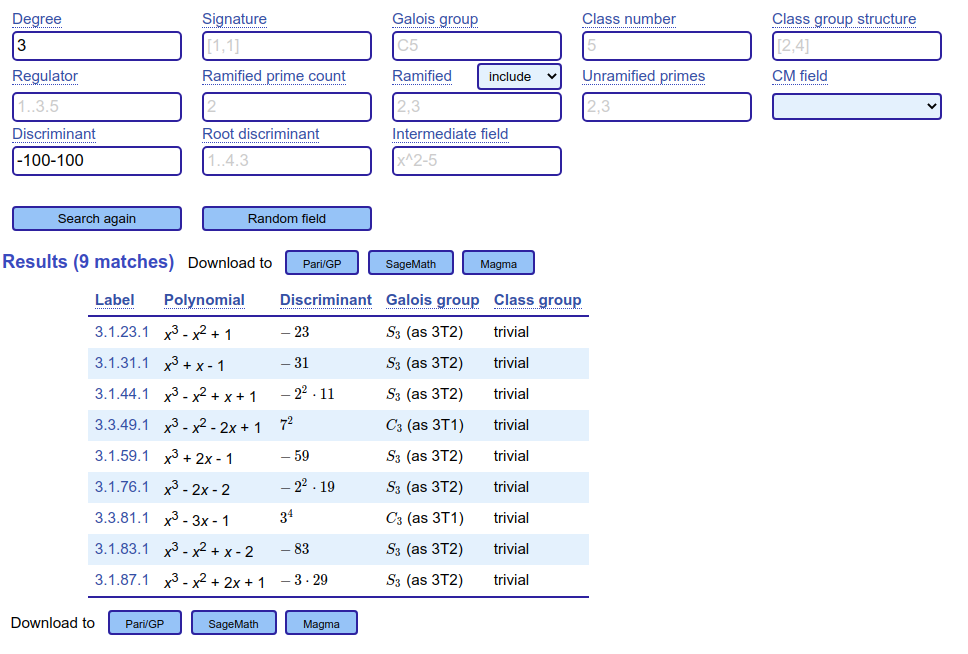
\includegraphics[width=12cm]{pic/lmfdb-cubic.png}}
  \end{center}
  
  \begin{center}
    \setlength{\fboxsep}{1pt}
    \setlength{\fboxrule}{0.5pt}
    \fbox{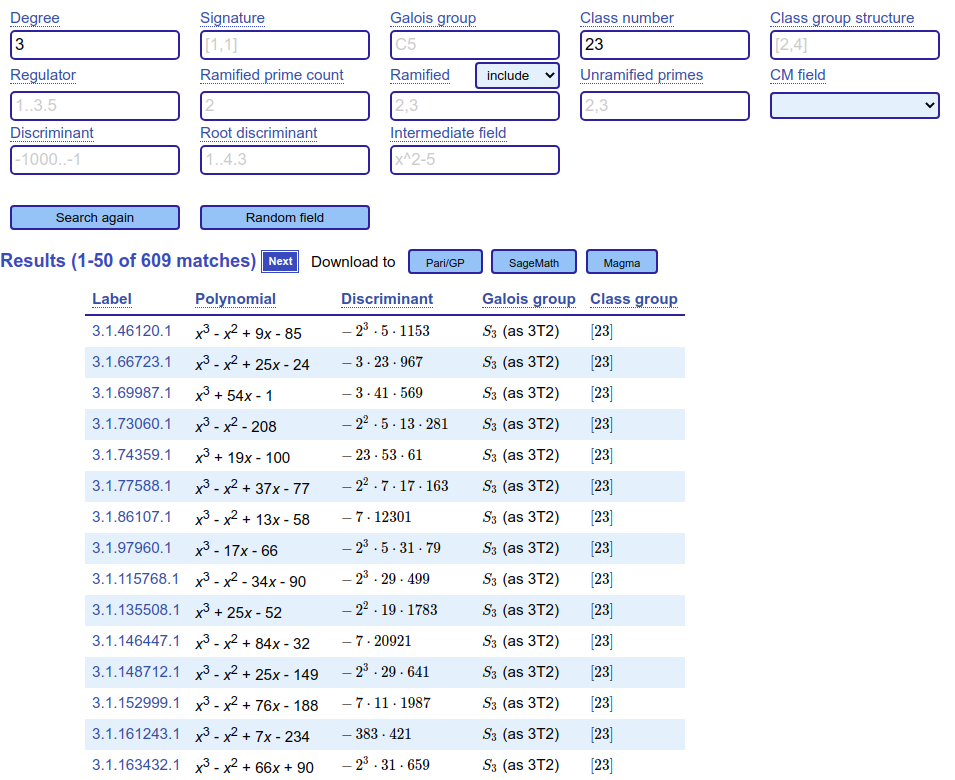
\includegraphics[width=12cm]{pic/lmfdb-23.png}}
  \end{center}

  \caption{Ejemplos de búsqueda en LMFDB:
    la lista completa de campos cúbicos con $|\Delta_K| \le 100$ y
    algunos campos cúbicos con $\Cl (K) \cong \ZZ/23\ZZ$}
\end{figure}

%%%%%%%%%%%%%%%%%%%%%%%%%%%%%%%%%%%%%%%%%%%%%%%%%%%%%%%%%%%%%%%%%%%%%%%%%%%%%%%%

\phantomsection

\addcontentsline{toc}{section}{Conclusión}
\section*{Conclusión}

En este capítulo investigamos los invariantes más importantes de un campo de
números $K/\QQ$: el grupo de clases $\Cl (K)$ y el grupo de unidades
$\O_K^\times$. Probamos que $\Cl (K)$ es un grupo finito, mientras que
$\O_K^\times$ es finitamente generado de rango $r_1 + r_2 - 1$. En general,
no es fácil encontrar generadores explícitos para $\O_K^\times$, pero vimos cómo
hacerlo en el caso especial cuando $K = \QQ (\sqrt{d})$ es un campo cuadrático
real. El siguiente capítulo será dedicado a los métodos analíticos,
en particular la \textbf{función zeta de Dedekind} $\zeta_K (s)$. La última
nos ayudará a relacionar $\Cl (K)$ con $\O_K^\times$, mediante la
\textbf{fórmula analítica del número de clases}, que es otro resultado
fundamental descubierto por Dirichlet (en el caso de campos cuadráticos,
y luego generalizado a todo $K/\QQ$ por Dedekind).

%%%%%%%%%%%%%%%%%%%%%%%%%%%%%%%%%%%%%%%%%%%%%%%%%%%%%%%%%%%%%%%%%%%%%%%%%%%%%%%%

\pagebreak

\phantomsection

\addcontentsline{toc}{section}{Ejercicios}
\section*{Ejercicios}

\begin{ejercicio}
  Demuestre que si $G$ es un grupo topológico Hausdorff, entonces todo subgrupo
  discreto $H \subset G$ es cerrado.
\end{ejercicio}

\begin{ejercicio}
  Demuestre directamente que $\ZZ [\sqrt{2}]$ no es un subgrupo discreto de
  $\RR$.
\end{ejercicio}

\begin{ejercicio}
  Demuestre que si $X$ es un conjunto convexo simétrico compacto tal que
  $\vol X = 2^n\cdot \covol \Lambda$, entonces $X \cap \Lambda \ne \{ 0 \}$.
\end{ejercicio}

\begin{ejercicio}
  Demuestre que para todo primo $p$ existen $m,n \in \ZZ$ tales que
  $m^2 + n^2 + 1 \equiv 0 \pmod{p}$.
\end{ejercicio}

\begin{ejercicio}
  Demuestre que
  $$a_n = \left(\frac{n^n}{n!}\right)^2\,\left(\frac{\pi}{4}\right)^n$$
  crece con $n$.
\end{ejercicio}

\begin{ejercicio}
  Para $t > 0$ consideremos el conjunto convexo simétrico
  $$X_t = \{ (x_\tau)_\tau \in K_\RR \mid |x_\tau| < t\text{ para todo }\tau \}.$$
  Calcule que
  $$\vol (X_t) = 2^{r_1}\,(2\pi)^{r_2}\,t^n.$$
\end{ejercicio}

\begin{ejercicio}
  Supongamos que $d = p_1\cdots p_s$, donde $s > 1$ y los $p_i$ son diferentes
  primos y consideremos el campo cuadrático imaginario $K = \QQ (\sqrt{-d})$.
  Demuestre que los ideales correspondientes
  $\mathfrak{p}_1,\ldots,\mathfrak{p}_s \subset \O_K$ generan un subgrupo en
  $\Cl (K)$ isomorfo a $(\ZZ/2\ZZ)^{s-1}$.
\end{ejercicio}

\begin{ejercicio}
  Calcule los grupos de clases de campos
  \[ \QQ (\sqrt{-110}), \quad
     \QQ (\sqrt{-127}), \quad
     \QQ (\sqrt{33}), \quad
     \QQ (\sqrt[3]{19}), \quad
     \QQ (\sqrt{-3}, \sqrt{-5}). \]
\end{ejercicio}

\begin{ejercicio}
  Sea $K/\QQ$ un campo de números. Demuestre que para cualquier ideal
  $I \subset \O_K$ existe una extensión finita $L/K$ tal que el ideal
  correspondiente $I\,\O_L$ es principal.

  \noindent (Use que $[I]$ tiene orden finito en $\Cl (K)$.)
\end{ejercicio}

\begin{ejercicio}
  \label{ejerc:seccion-de-sec}
  Consideremos una sucesión exacta corta de $R$-módulos
  $$0 \to M' \xrightarrow{i} M \xrightarrow{p} M'' \to 0$$

  \begin{enumerate}
  \item[1)] Demuestre que si $M''$ es un $R$-módulo libre, entonces
    el homomorfismo $p$ admite una \textbf{sección} $s\colon M'' \to M$
    tal que $p\circ s = id_{M''}$.

  \item[2)] Demuestre si existe una sección $s$ como arriba, entonces
    $M'\oplus M'' \cong M$.
  \end{enumerate}
\end{ejercicio}

\begin{ejercicio}
  Encuentre el número cuadrático $\alpha$ tal que
  $\alpha = [3, \overline{2,1}]$.
\end{ejercicio}

\begin{ejercicio}
  Demuestre que si $\alpha = [a_0,a_1,a_2,\ldots]$, entonces
  $\frac{1}{\alpha} = [0,a_0,a_1,a_2,\ldots]$. Concluya que si las fracciones
  parciales para $\alpha$ y $\frac{1}{\alpha}$ son $\frac{p_n}{q_n}$ y
  $\frac{p_n'}{q_n'}$ respectivamente, entonces
  $\frac{p_n'}{q_n'} = \frac{q_{n-1}}{p_{n-1}}$.
\end{ejercicio}

\begin{ejercicio}
  Encuentre las fracciones continuas para $\sqrt{n^2+1}$, $\sqrt{n\,(n+1)}$,
  $\sqrt{m^2\,n^2 + n}$.
\end{ejercicio}

\begin{ejercicio}
  Describa el grupo de unidades $\O_K^\times$ para $K = \QQ (\sqrt{29})$
  (justifique todos los cálculos sin usar las tablas).
\end{ejercicio}
